\newpage

\section{Results and discussion}
\label{Sec:Results}

In this section, the results of the \pT-dependent non-linear flow modes $v_{4,22}$, $v_{5,32}$, $v_{6,33}$ and $v_{6,222}$ of identified particles are presented for various centrality intervals in Pb--Pb collisions at \sNN. We first present the centrality and \pT~dependence of $v_{n,mk}$ in Sec. \ref{SubSec:pTdependence}. The scaling properties of non-linear flow modes are also discussed in this section. These results are compared with $v_{n}$ measurements for the same particle species in Sec. \ref{SubSec:comparewithvn}. Finally, the comparison to two model calculations is shown in Sec. \ref{SubSec:hydro}. Note that in some of the following sections the same data are used in different representations to highlight the various physics implications of the measurements in each section.

%~for 0-5\% up to 50-60\% centrality intervals for \pion, \kaon, \proton, \Ks, \lambdas~and $\phi$-meson

\subsection{Centrality and \pT~dependence of non-linear flow modes}
\label{SubSec:pTdependence}

%Higher order flow coefficients are mainly generated by inhomogeneities in the initial density profile and the collision geometry. 
Figure \ref{v422_centralityDependence} presents the magnitude of the non-linear mode for the fourth order flow coefficient, $v_{4,22}(p_{\rm{T}})$, for \pion, \kaon,\Ks, \proton, \lambdas~and $\phi$-meson in a wide range of centrality intervals, i.e. 0-5\% up to 50-60\%. For the $\phi$-meson, the results are reported from 10-20\% up to 40-50\% centrality interval, where $v_{4,22}$ can be measured accurately. The magnitude of this non-linear flow mode rises steeply with increasing centrality interval from 0-5\% to 40-50\% for all particle species. This increase is expected as $v_{4,22}$ reflects the contribution of the second order eccentricity, $\varepsilon_{2}$, which increases from central to peripheral collisions, in $v_{4}$ \cite{Alver:2010gr, Acharya:2017zfg}. For more peripheral collisions (i.e. 50-60\%) , the magnitude of $v_{4,22}$ is smaller than in the previous centrality intervals for all particle species. This effect that was observed also in $v_n$ measurements is probably due to the shorter lifetime of the produced system in more peripheral collisions, which prevents $v_{4,22}$ from developing further. 


\begin{figure}[!htb]
\begin{center}
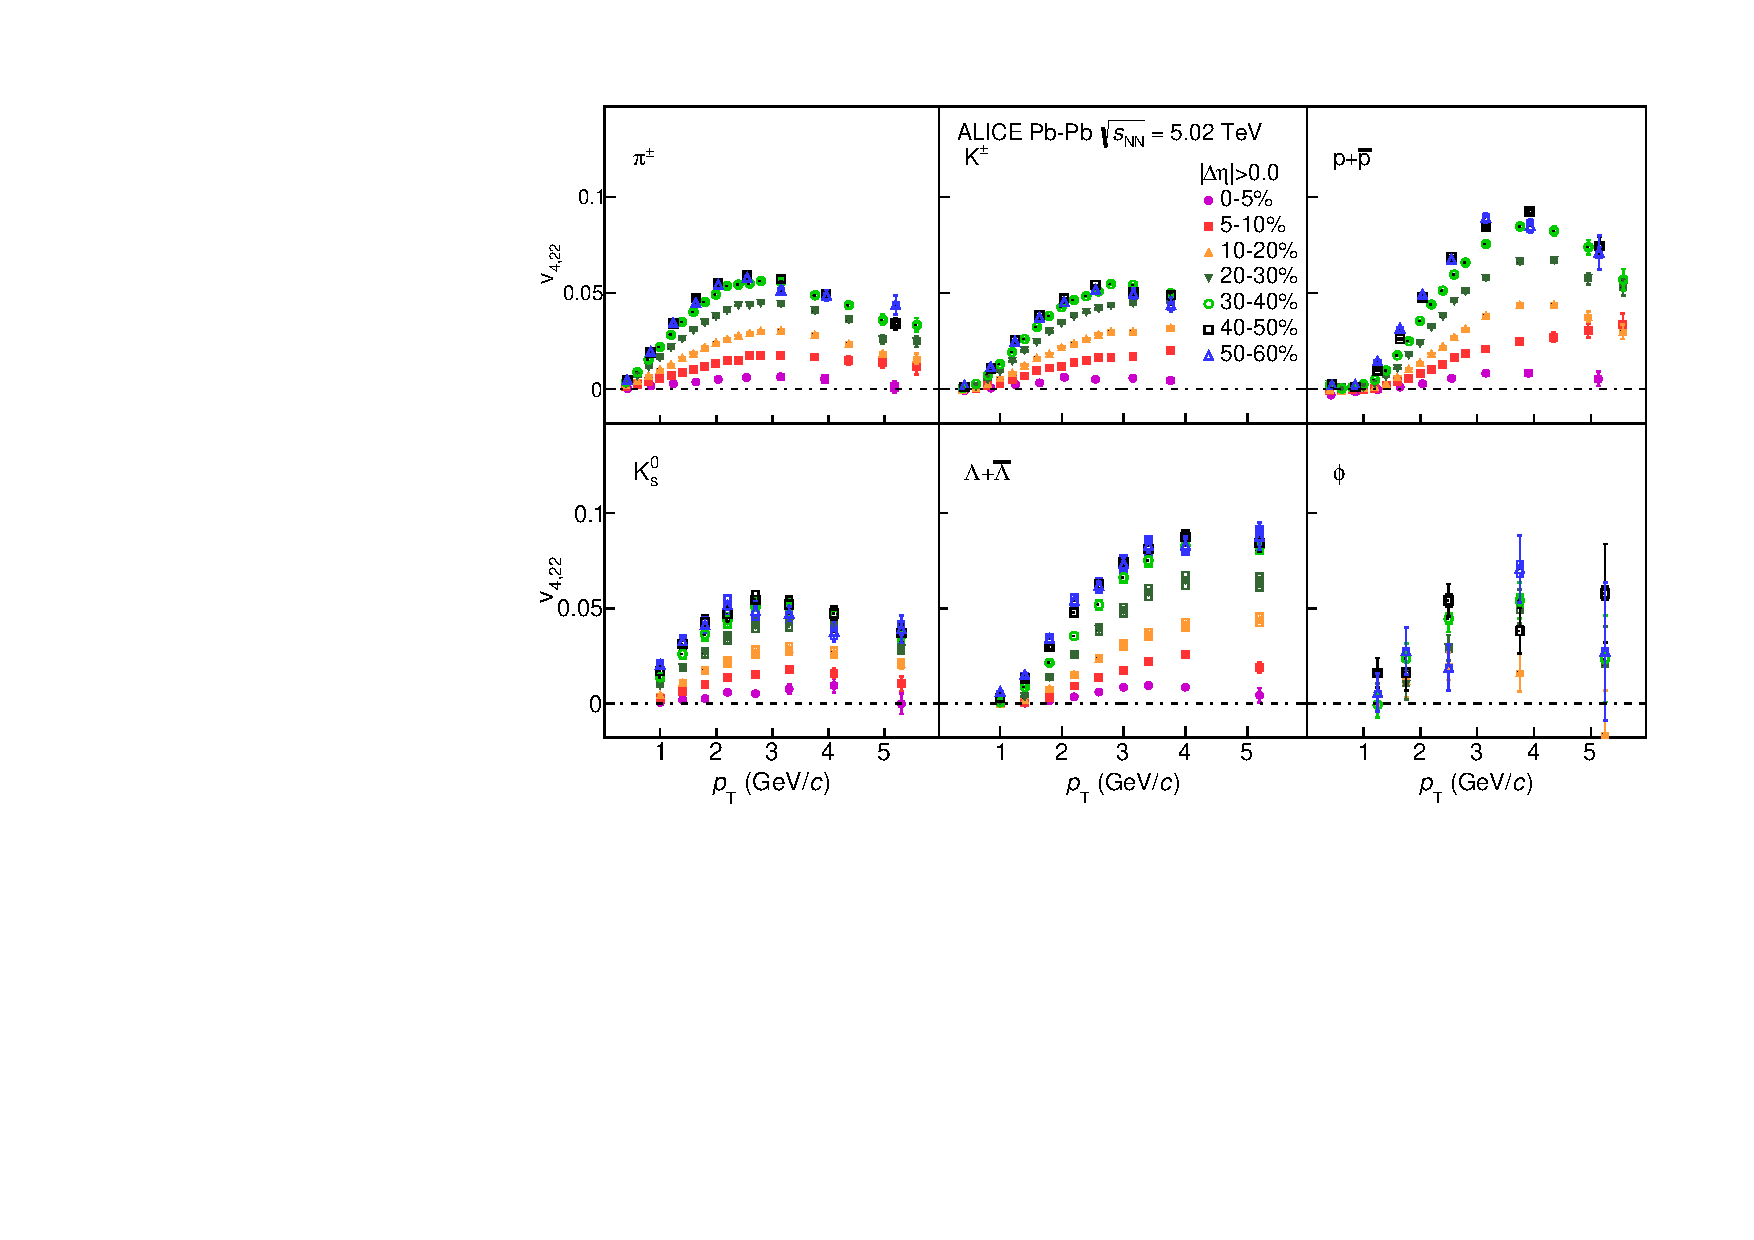
\includegraphics[scale=0.82]{figures/results/All_v422_gap00_CentDep_PID2.pdf}
\end{center}
\caption{The \pT-differential $v_{4,22}$ for different centrality intervals of Pb--Pb collisions at \sNN~ grouped by particle species. Statistical and systematic uncertainties are shown as bars and boxes, respectively.}
\label{v422_centralityDependence}
\end{figure}
 
Figure \ref{v523_centralityDependence} presents the non-linear mode for the fifth order flow coefficient, i.e. $v_{5,32}(p_{\rm{T}})$, of \pion, \kaon, \Ks, \proton, and \lambdas~for the same range of centrality intervals, i.e. 0-5\% up to 50-60\%. Statistical precision limits extending the measurements of non-linear flow modes of $\phi$-meson for $n>4$. The measurements show a significant increase in the magnitude of this non-linear flow mode with increasing centrality percentile. This is due to the fact that $v_{5,32}(p_{\rm{T}})$ has a contribution from both $\varepsilon_{2}$ and $\varepsilon_{3}$. It is shown in MC studies that $\varepsilon_{2}$ and to a smaller extent, $\varepsilon_{3}$ increase for peripheral collisions \cite{Alver:2010gr}. 

\begin{figure}[!htb]
\begin{center}
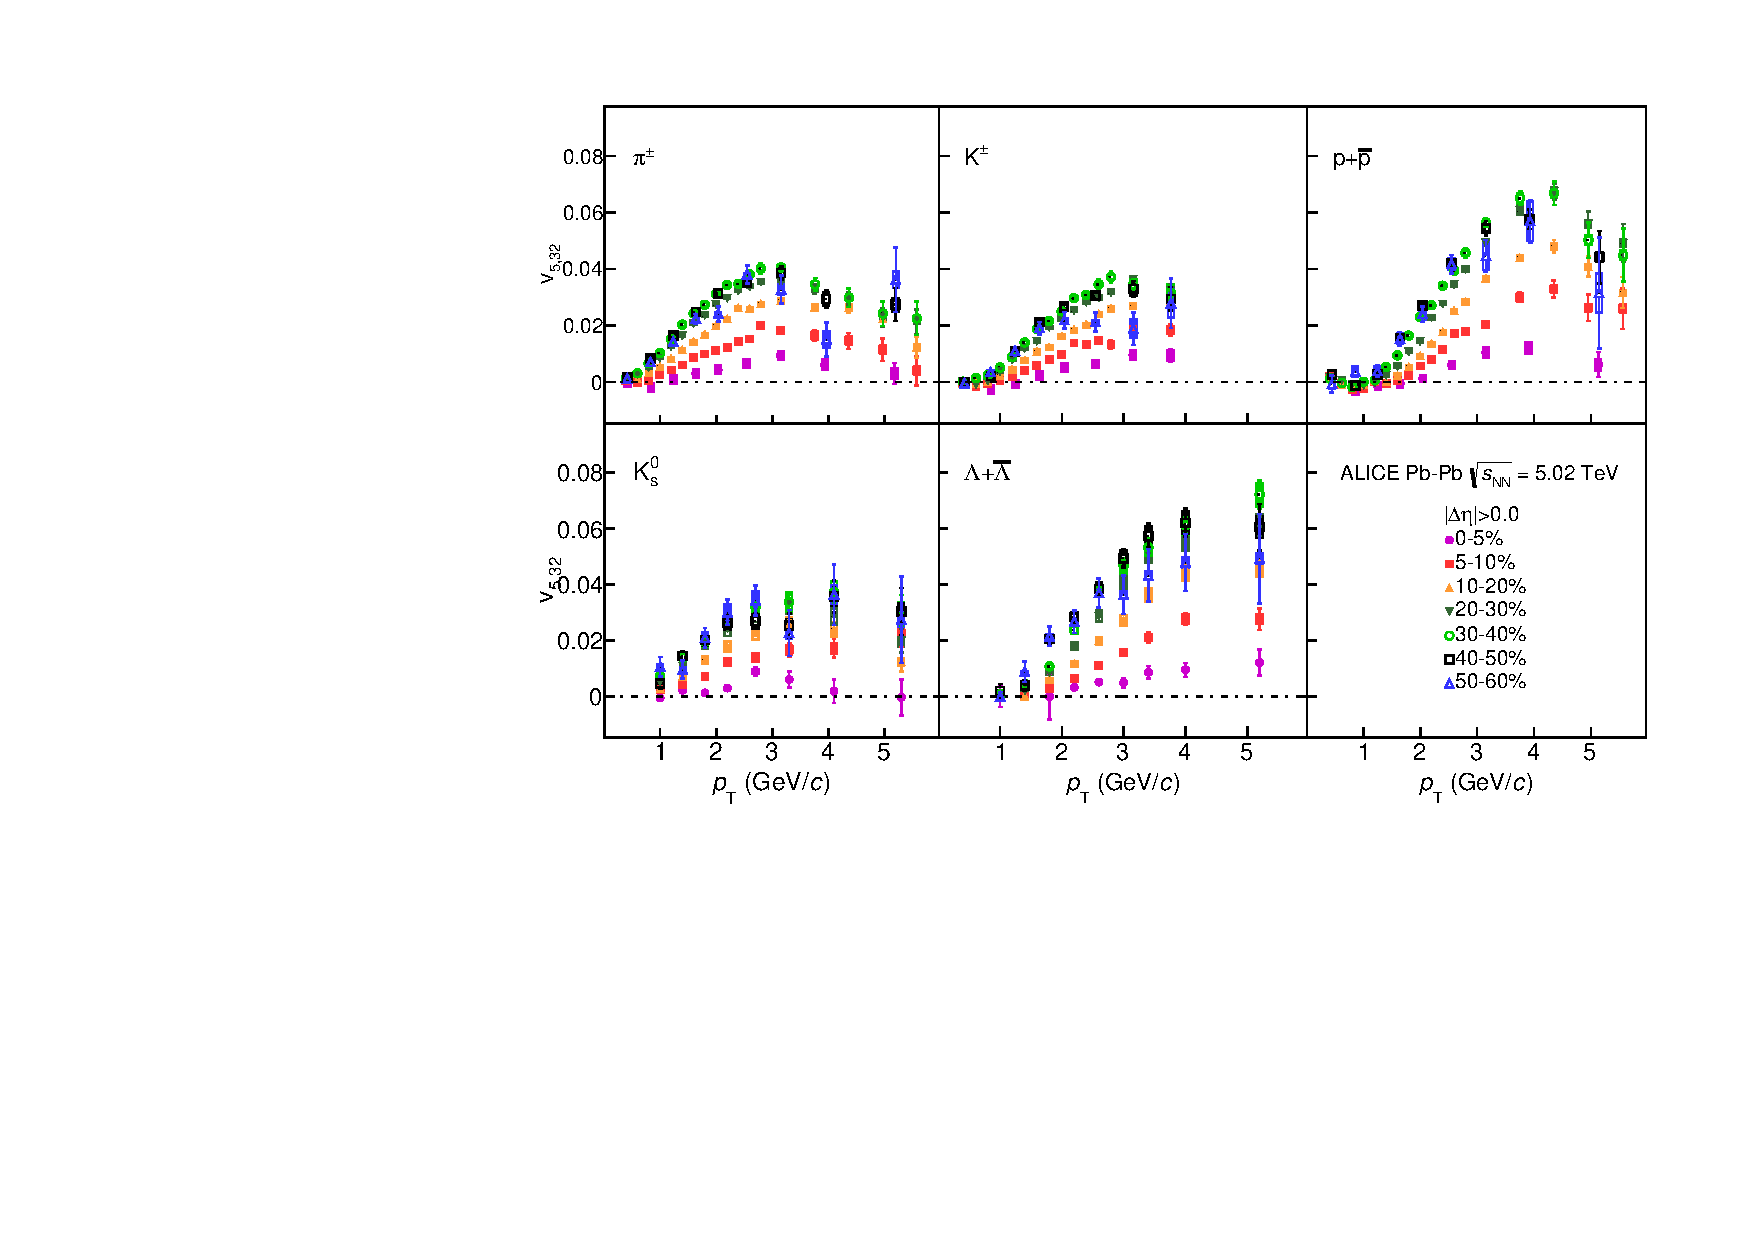
\includegraphics[scale=0.82]{figures/results/All_v523_gap00_CentDep_PID2.pdf}
\end{center}
\caption{The \pT-differential $v_{5,32}$ for different centrality intervals of Pb--Pb collisions at \sNN~ grouped by particle species.}
\label{v523_centralityDependence}
\end{figure}

Figures \ref{v633_centralityDependence} and \ref{v6222_centralityDependence} present the non-linear terms for the sixth order flow coefficient, i.e. $v_{6,33}(p_{\rm{T}})$ for \pion, \kaon, \Ks, \proton~and \lambdas~at 0-5\% up to 40-50\% centrality intervals and $v_{6,222}(p_{\rm{T}})$ for \pion, \kaon, \proton~at 0-5\% up to 50-60\% centrality intervals. As expected, measurements of $v_{6,222}(p_{\rm{T}})$ which probe the contribution of $\varepsilon_2$, show an increase in the magnitude of this non-linear flow mode with increasing centrality percentile. On the other hand, $v_{6,33}(p_{\rm{T}})$ measurements, which probe the contribution of $\varepsilon_3$, present little to no dependence on centrality \cite{Acharya:2017zfg}. 

\begin{figure}[!htb]
\begin{center}
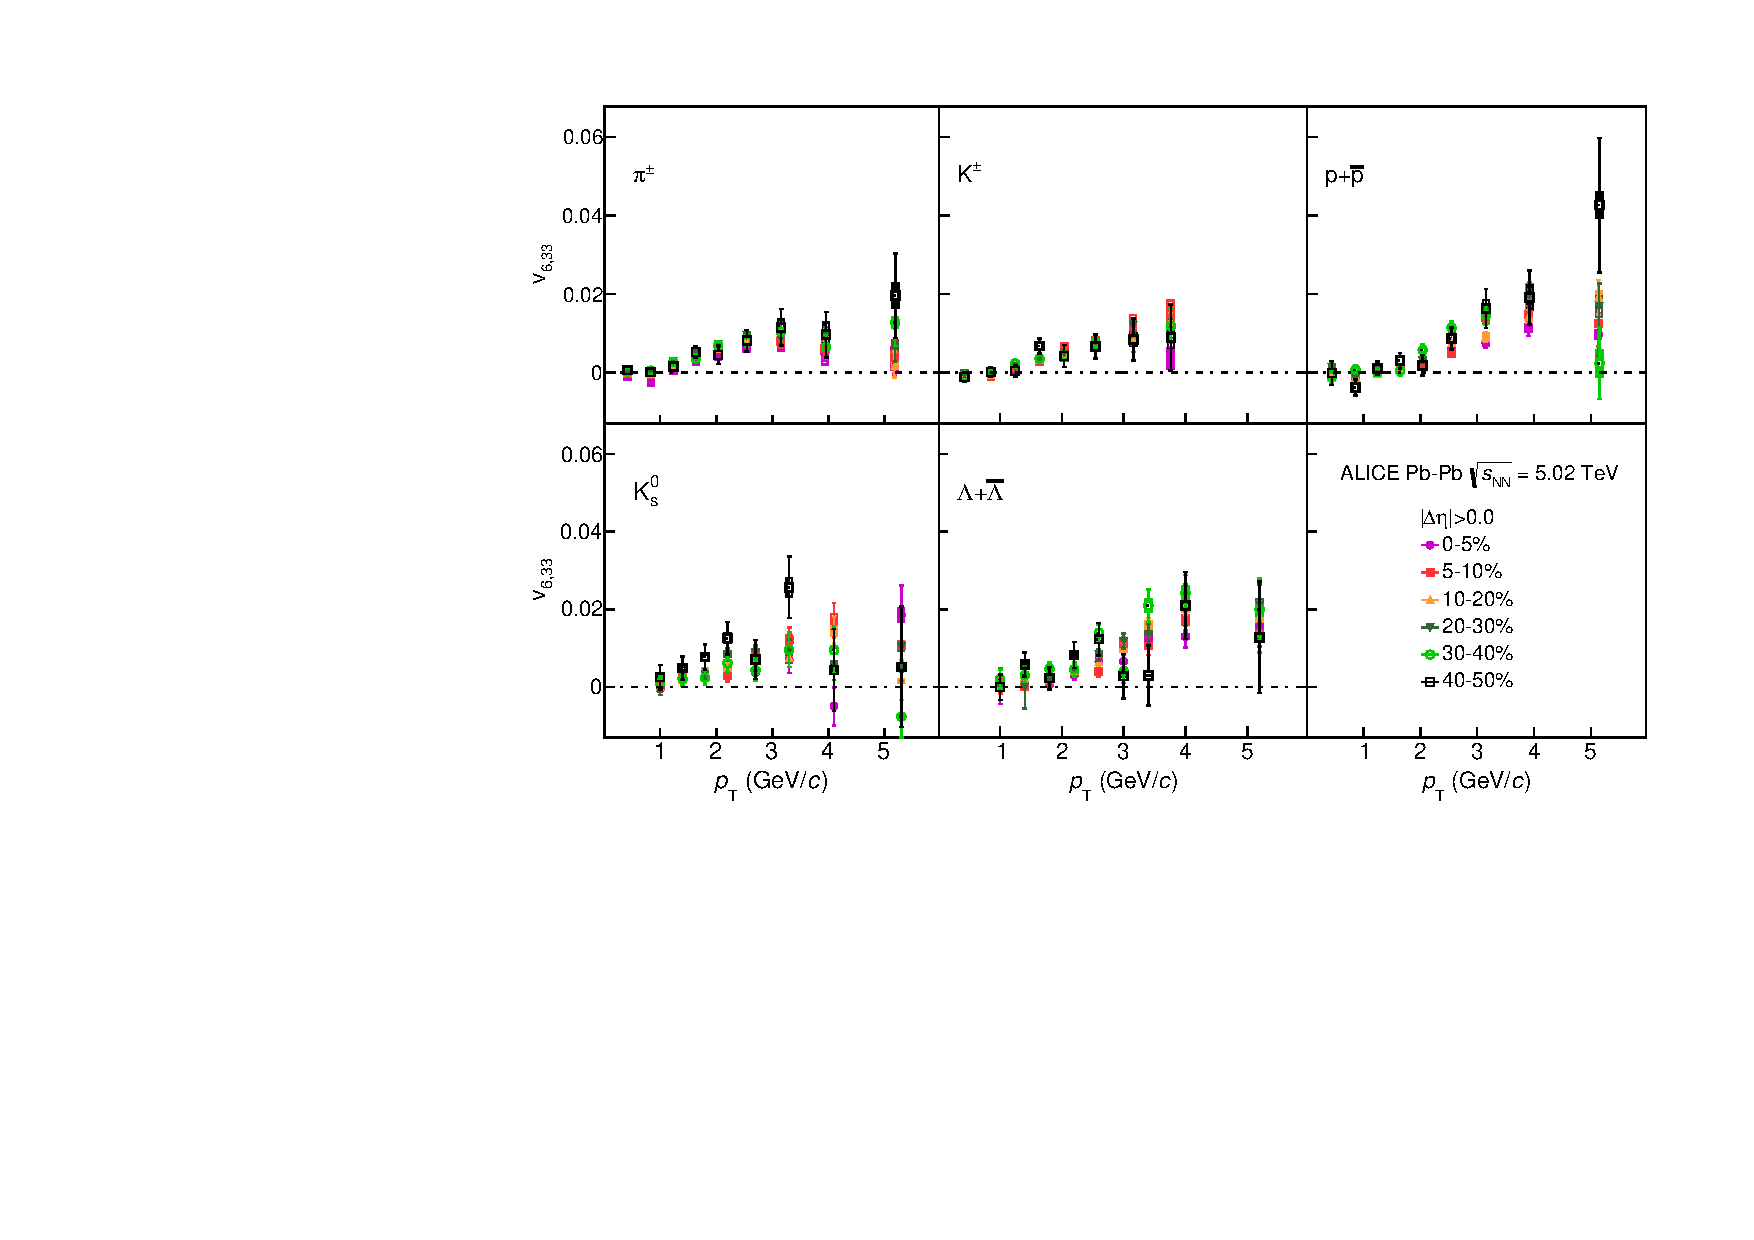
\includegraphics[scale=0.82]{figures/results/All_v633_gap00_CentDep_PID2.pdf}
\end{center}
\caption{The \pT-differential $v_{6,33}$ for different centrality intervals of Pb--Pb collisions at \sNN~ grouped by particle species.}
\label{v633_centralityDependence}
\end{figure}

\begin{figure}[!htb]
\begin{center}
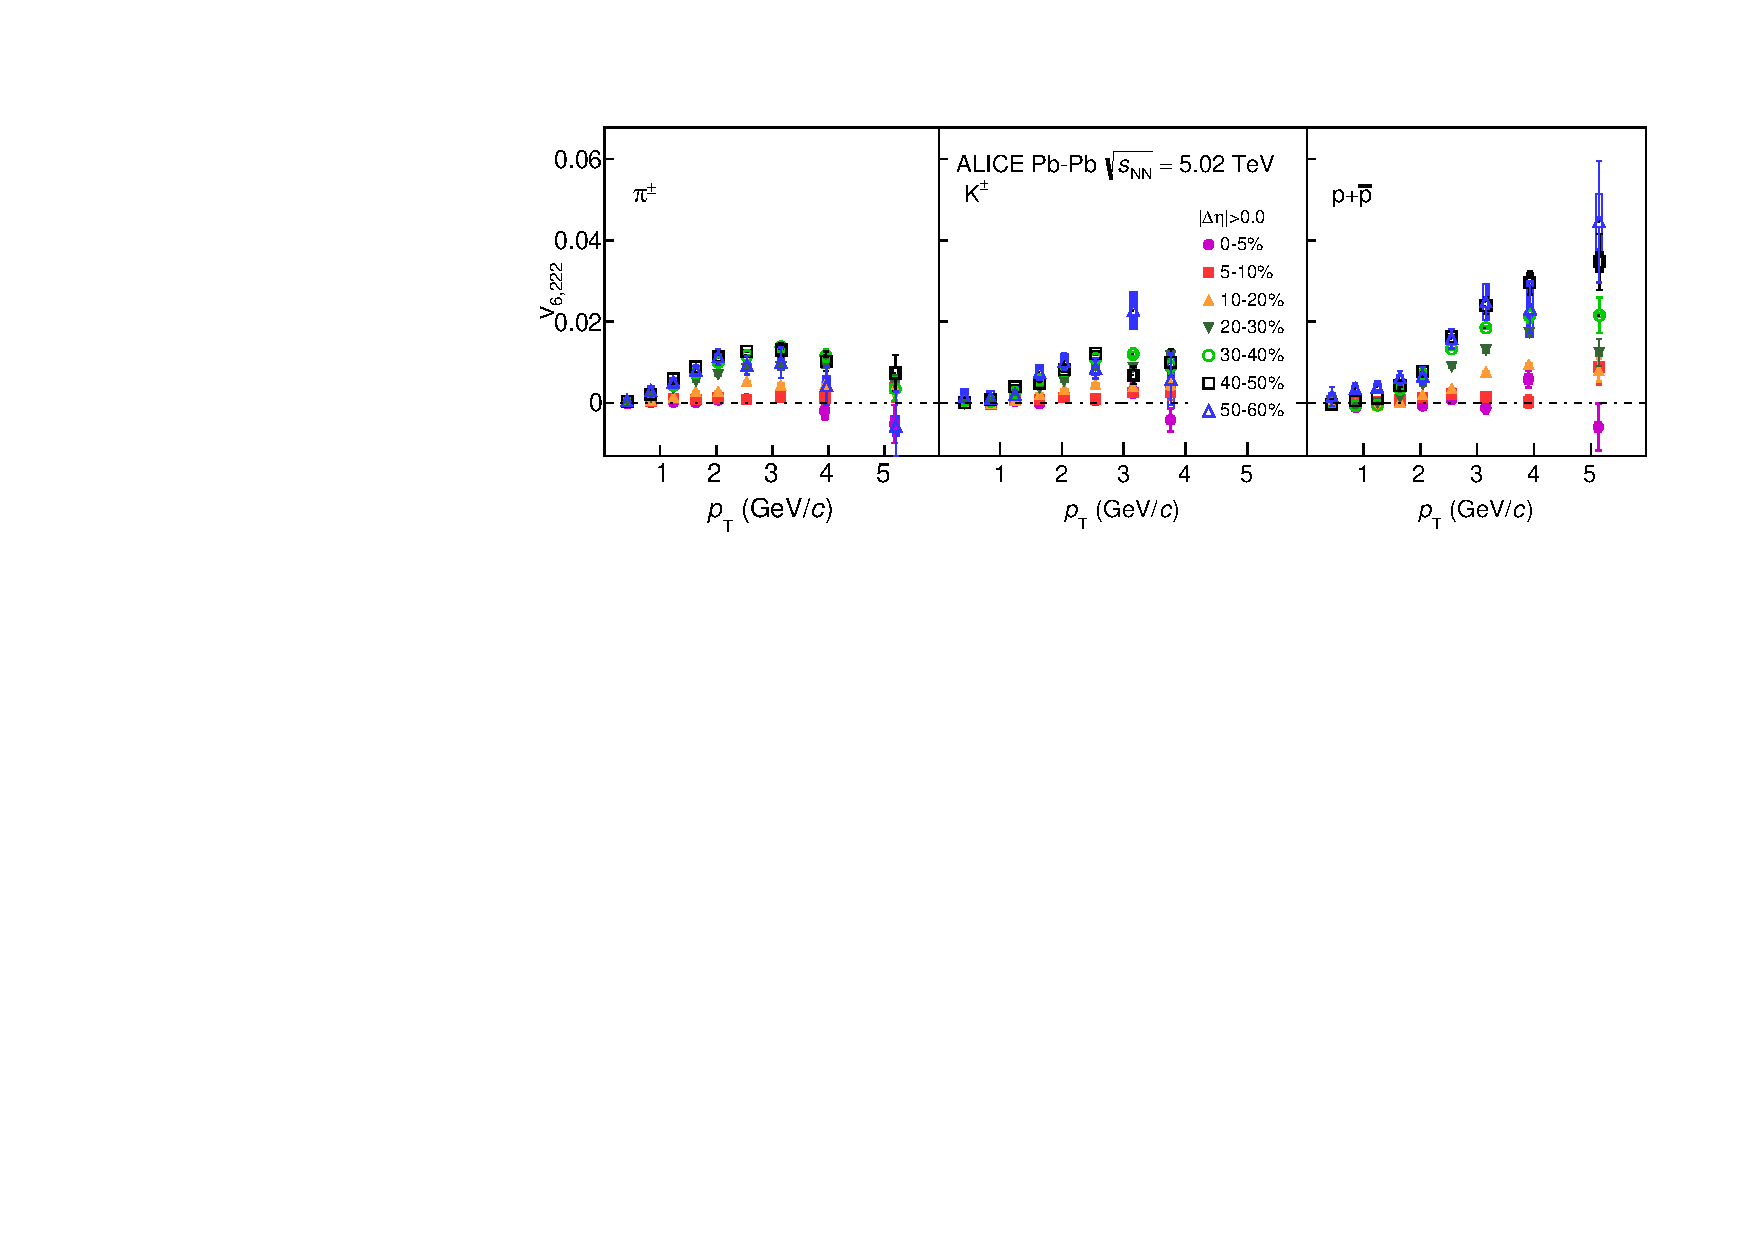
\includegraphics[scale=0.82]{figures/results/All_v6222_gap00_CentDep_PID2.pdf}
\end{center}
\caption{The \pT-differential $v_{6,222}$ for different centrality intervals of Pb--Pb collisions at \sNN~ grouped by particle species.}
\label{v6222_centralityDependence}
\end{figure}

\newpage
%\subsection{Mass ordering}
%\label{MassOrdering}

In Fig. \ref{v422_particleDependence} the same data points are grouped by centrality interval to highlight how $v_{4,22}$ develops for a given centrality for various particle species as a function of \pT.
%Figures \ref{v422_particleDependence} presents the \pT-differential $v_{4,22}$ for \pion, \kaon, \proton, \Ks, \lambdas~and $\phi$-meson starting from most central collisions (0-5\%) up to the 50-60\% centrality interval. 
A clear mass ordering can be seen in the low \pT~region (i.e. \pT $< 2.5$ \GeV) for all collision centralities. This mass ordering arises from the interplay between radial flow and the initial spatial anisotropy, created from both the geometry and the fluctuating initial energy density profile. This creates a depletion in the particle spectra at lower \pT~values which becomes larger in-plane than out-of plane due to the velocity profile. This naturally leads to lower $v_{4,22}$(\pT) for heavier particles \cite{Voloshin:1996nv, Huovinen:2001cy, Shen:2011eg}. Similarly, Figs. \ref{v523_particleDependence}, \ref{v633_particleDependence} and \ref{v6222_particleDependence} show the \pT-differential $v_{5,32}$, $v_{6,33}$ and $v_{6,222}$ respectively, of different particle species for each centrality interval. A clear mass ordering is seen in the low \pT~region, (i.e. \pT $< 2.5$ \GeV), for $v_{5,32}(p_{\rm{T}})$, $v_{6,33}(p_{\rm{T}})$ and $v_{6,222}(p_{\rm{T}})$.%, which similarly arises from the interplay between radial flow and initial spatial anisotropy. 

%This creates a depletion in particle spectra at lower pt, larger in in-plane than out-of plane. In its turn this lead to lower vn(pt) values for heavier particles.

\begin{figure}[!htb]
\begin{center}
%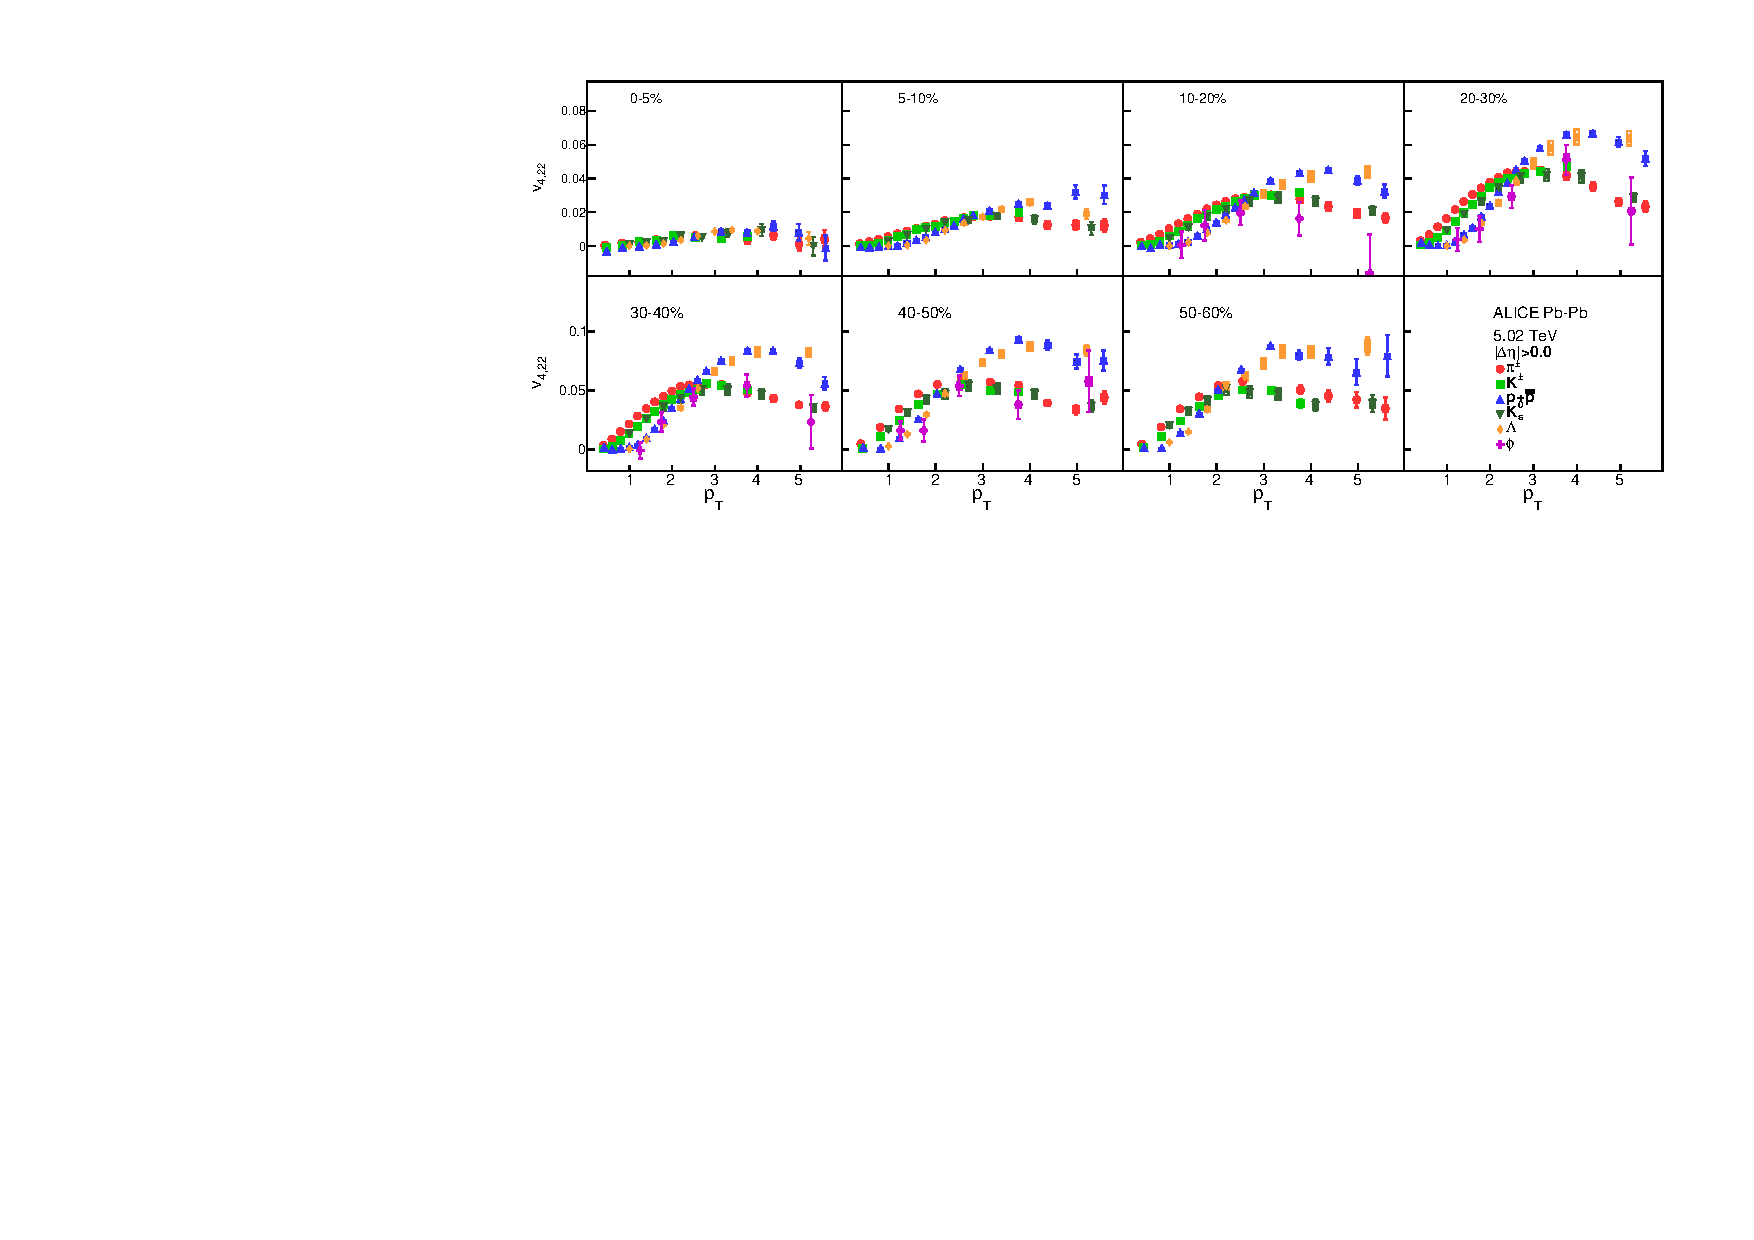
\includegraphics[scale=0.82]{figures/results/All_v422_gap00.pdf}
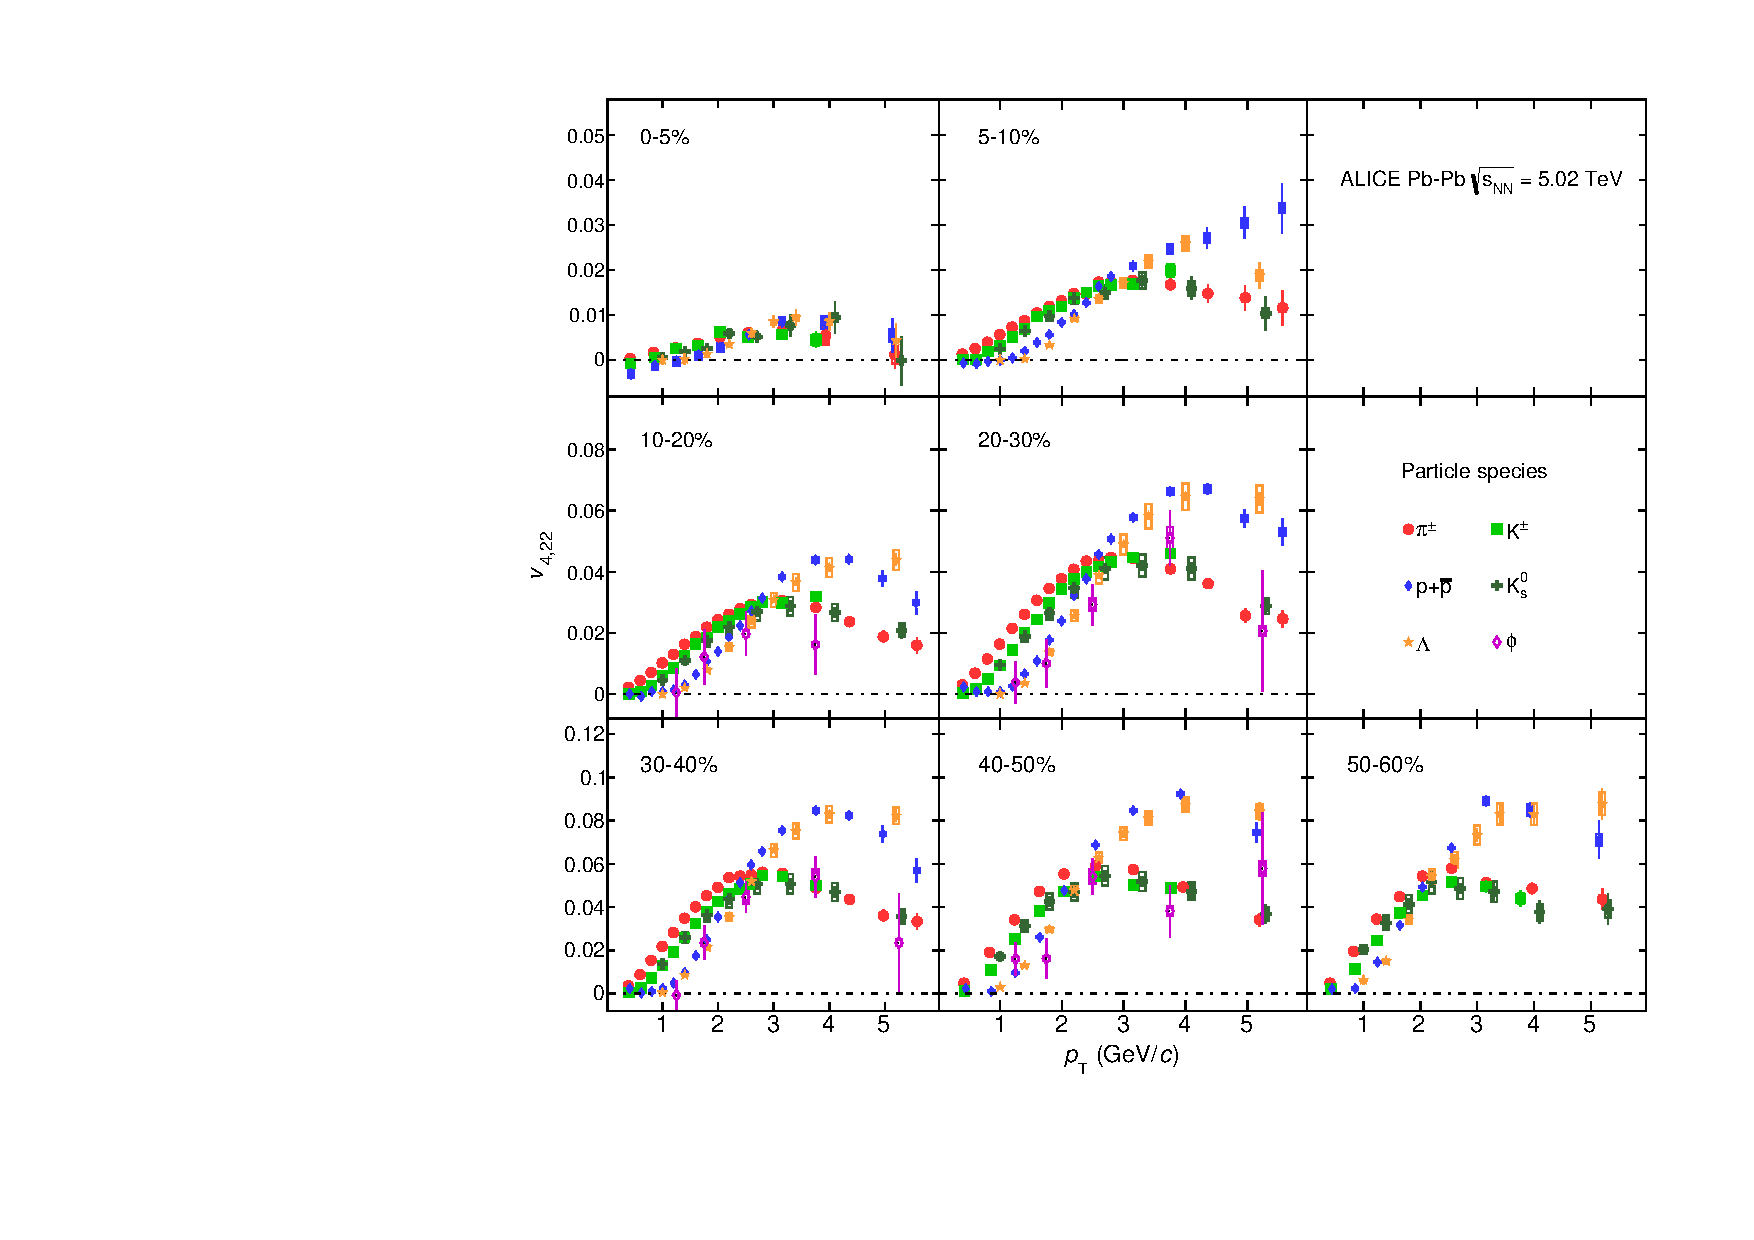
\includegraphics[scale=0.82]{figures/results/All_v422_gap00_PID2_3by3.pdf}
\end{center}
\caption{The \pT-differential $v_{4,22}$ for different particle species grouped into different centrality intervals of Pb--Pb collisions at \sNN.}
\label{v422_particleDependence}
\end{figure}

\begin{figure}[!htb]
\begin{center}
%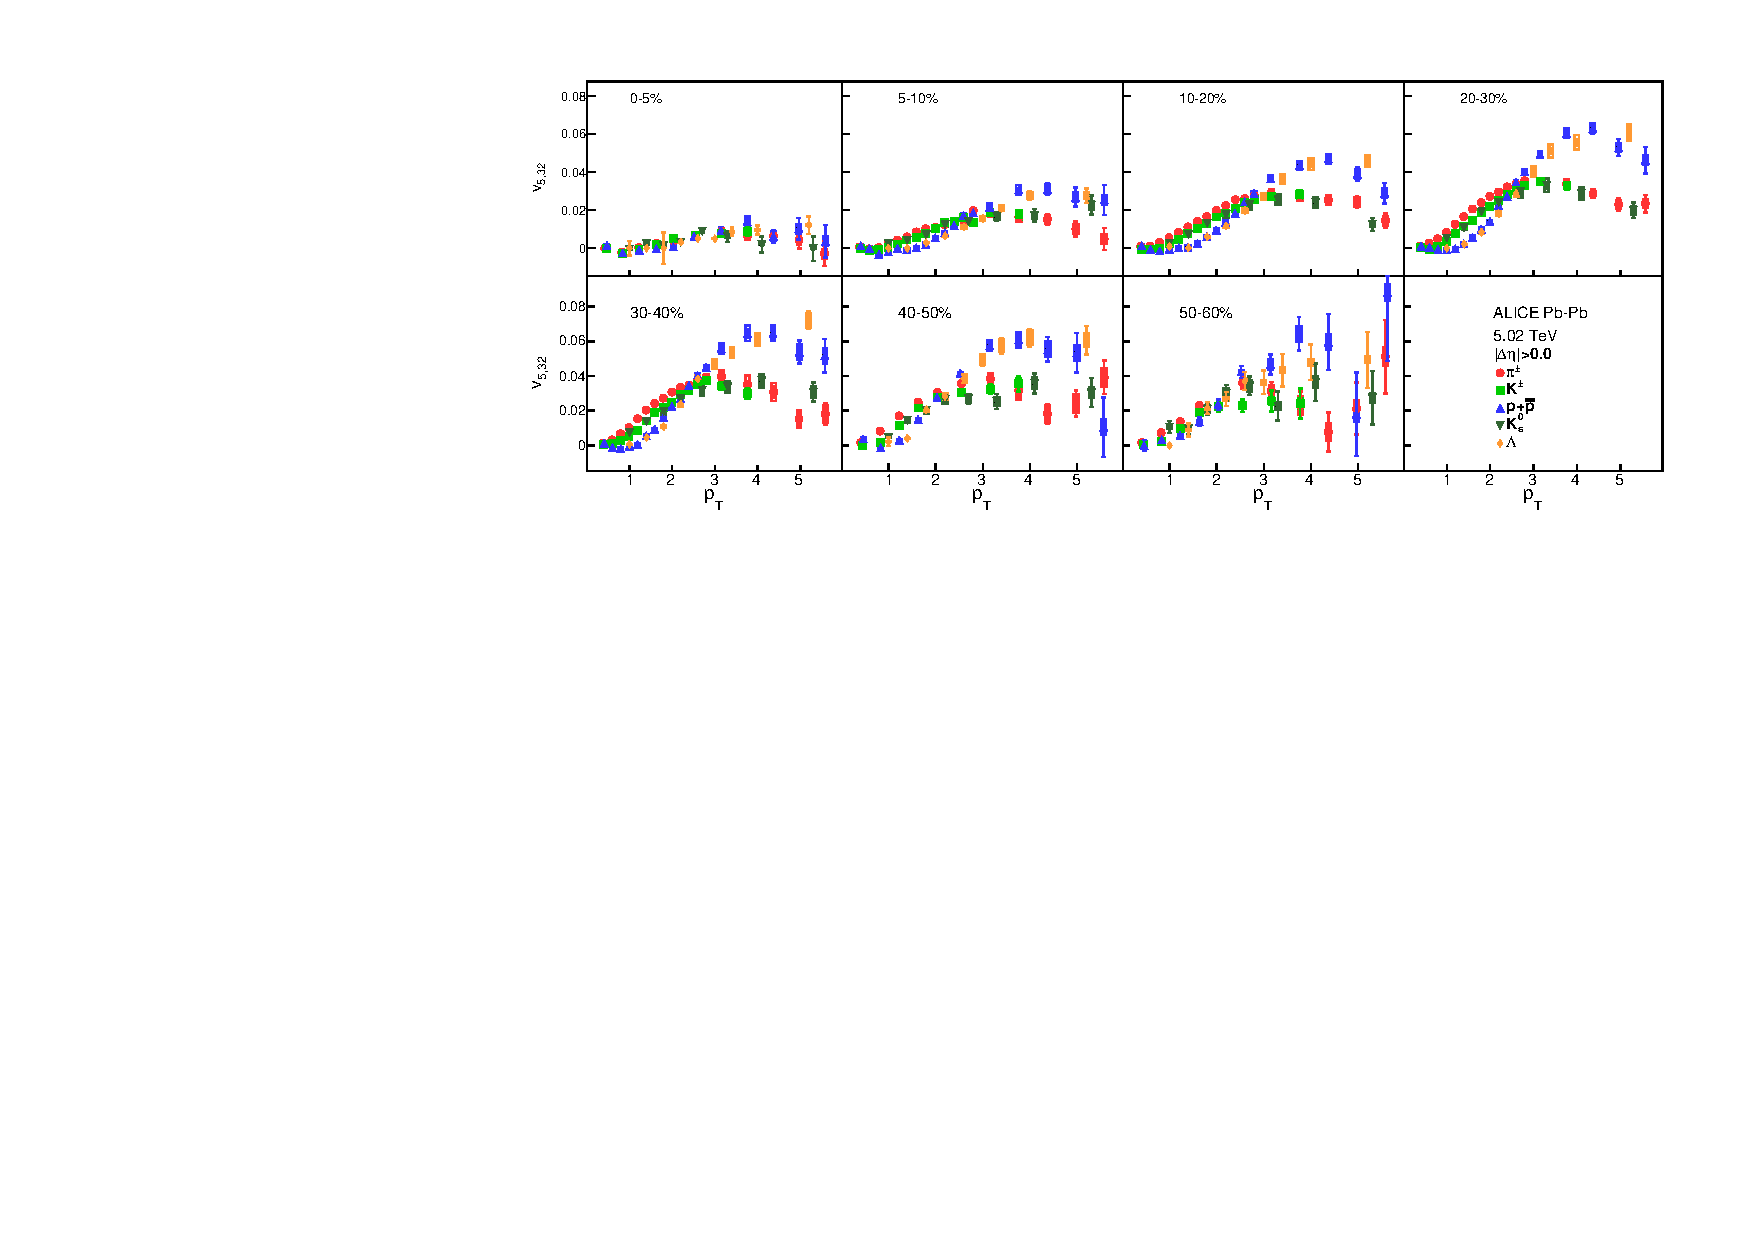
\includegraphics[scale=0.82]{figures/results/All_v523_gap00.pdf}
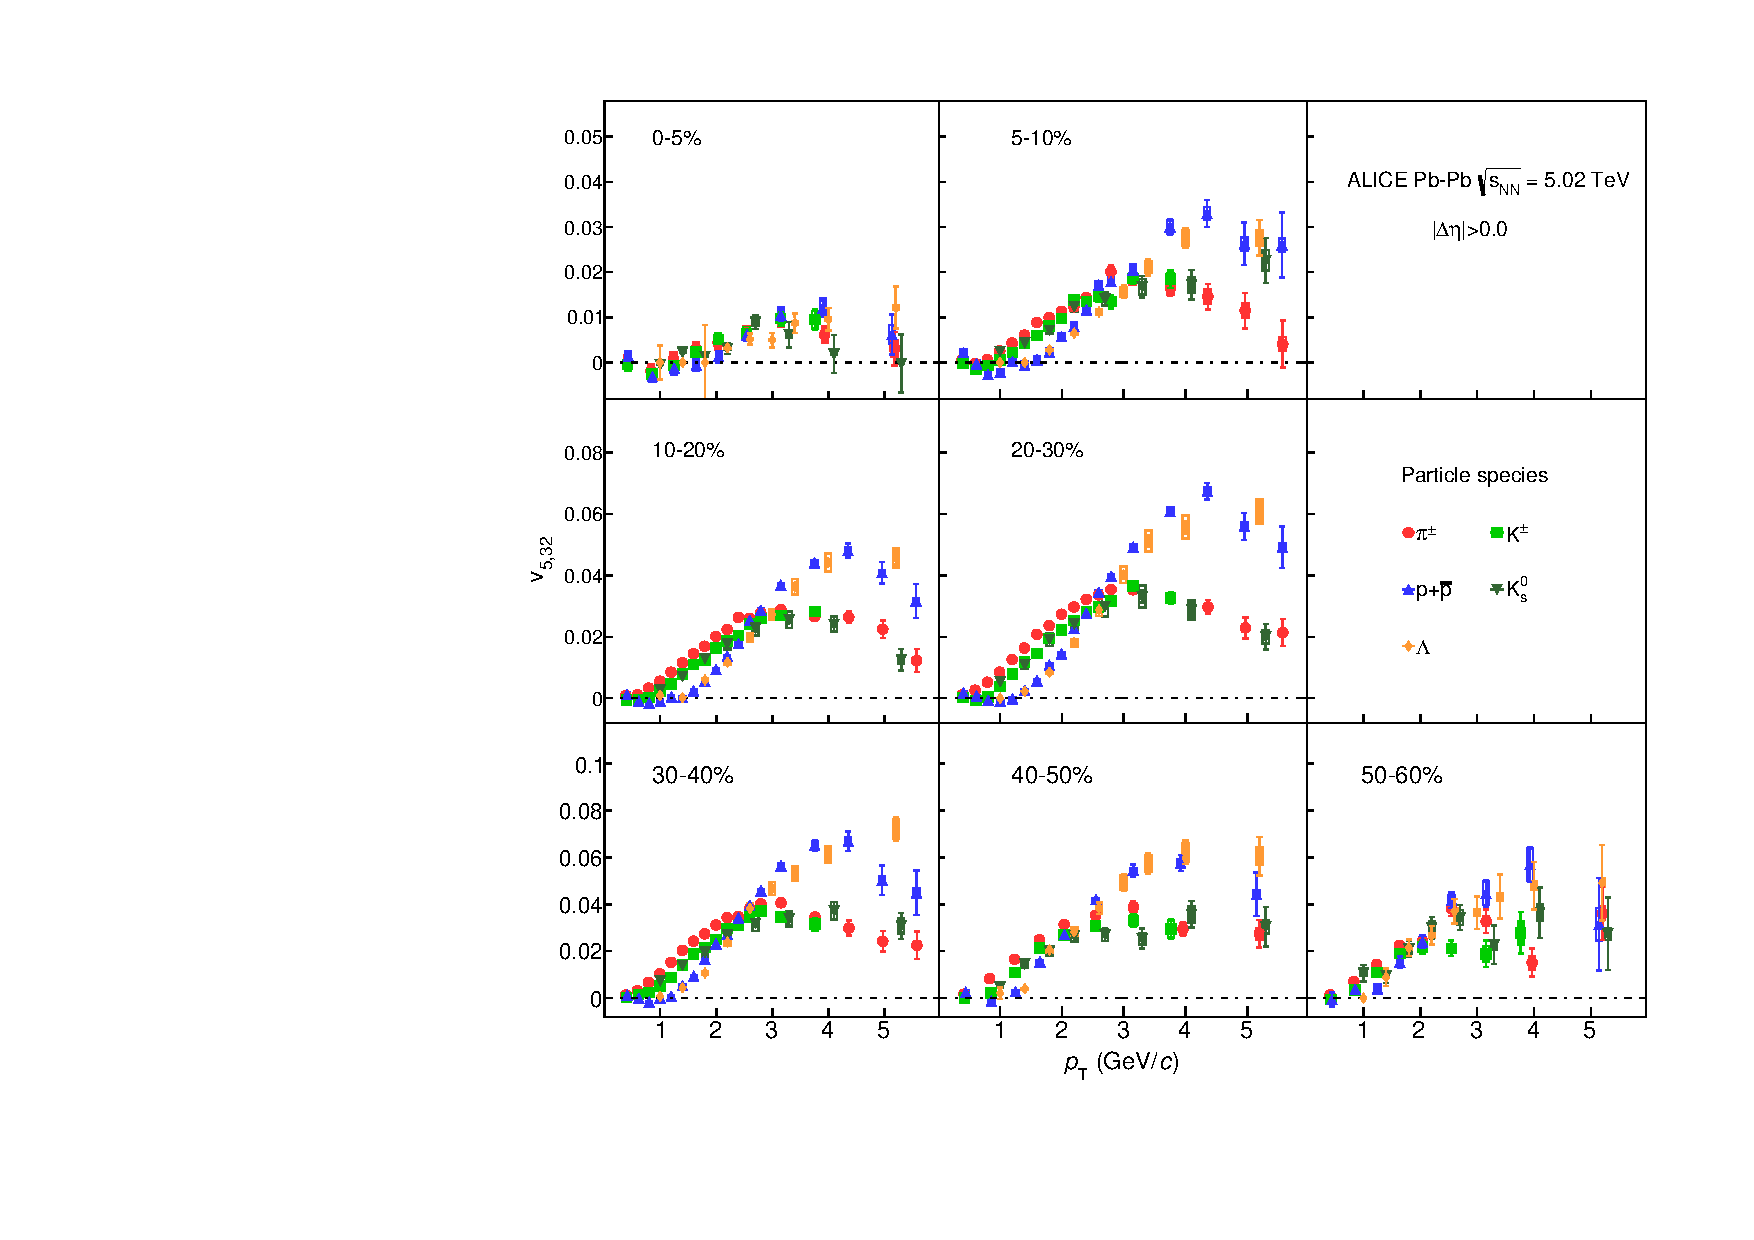
\includegraphics[scale=0.82]{figures/results/All_v523_gap00_PID2_3by3.pdf}

\end{center}
\caption{The \pT-differential $v_{5,32}$ for different particle species grouped into different centrality intervals of Pb--Pb collisions at \sNN.}
\label{v523_particleDependence}
\end{figure}

\begin{figure}[!htb]
\begin{center}
%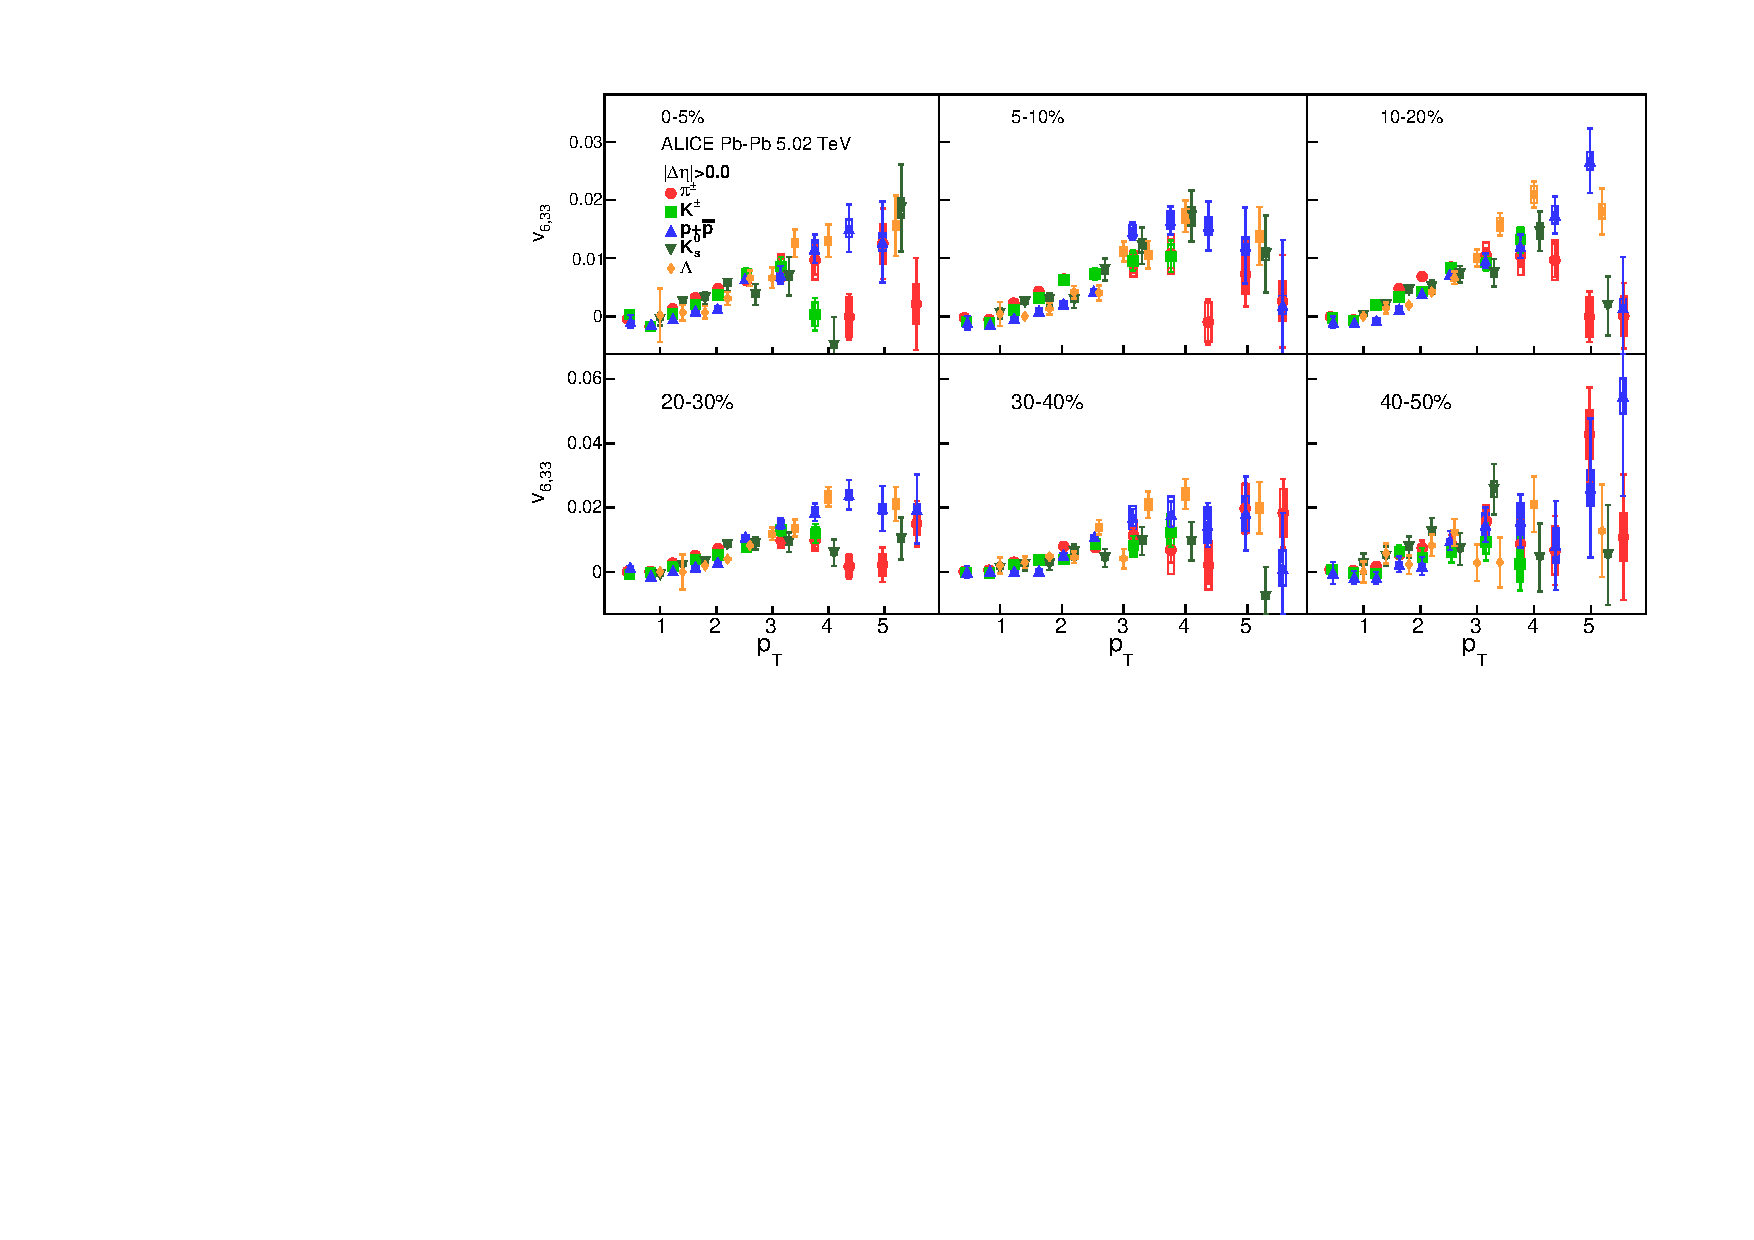
\includegraphics[scale=0.62]{figures/results/All_v633_gap00.pdf}
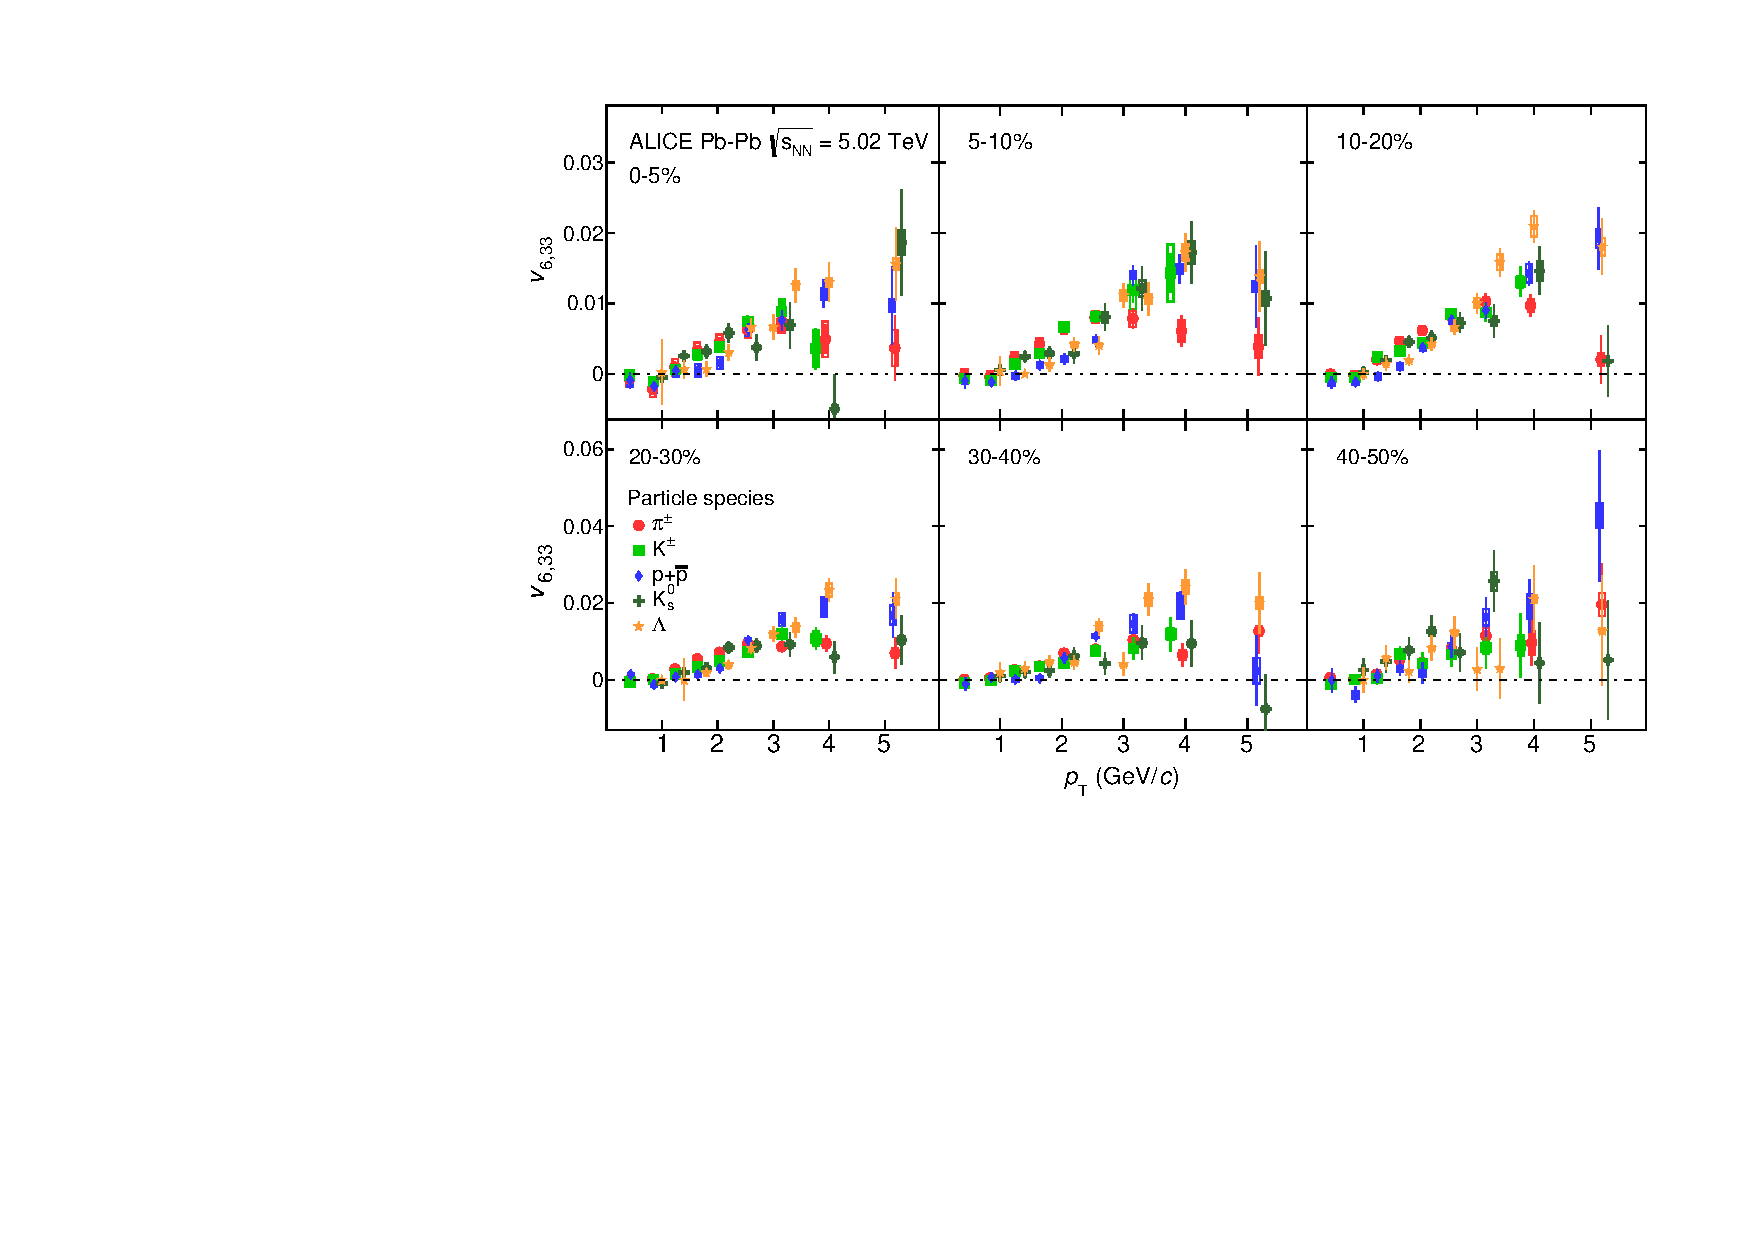
\includegraphics[scale=0.82]{figures/results/All_v633_gap00_PID2_3by2.pdf}

\end{center}
\caption{The \pT-differential $v_{6,33}$ for different particle species grouped into different centrality intervals of Pb--Pb collisions at \sNN.}
\label{v633_particleDependence}
\end{figure}

\begin{figure}[!htb]
\begin{center}
%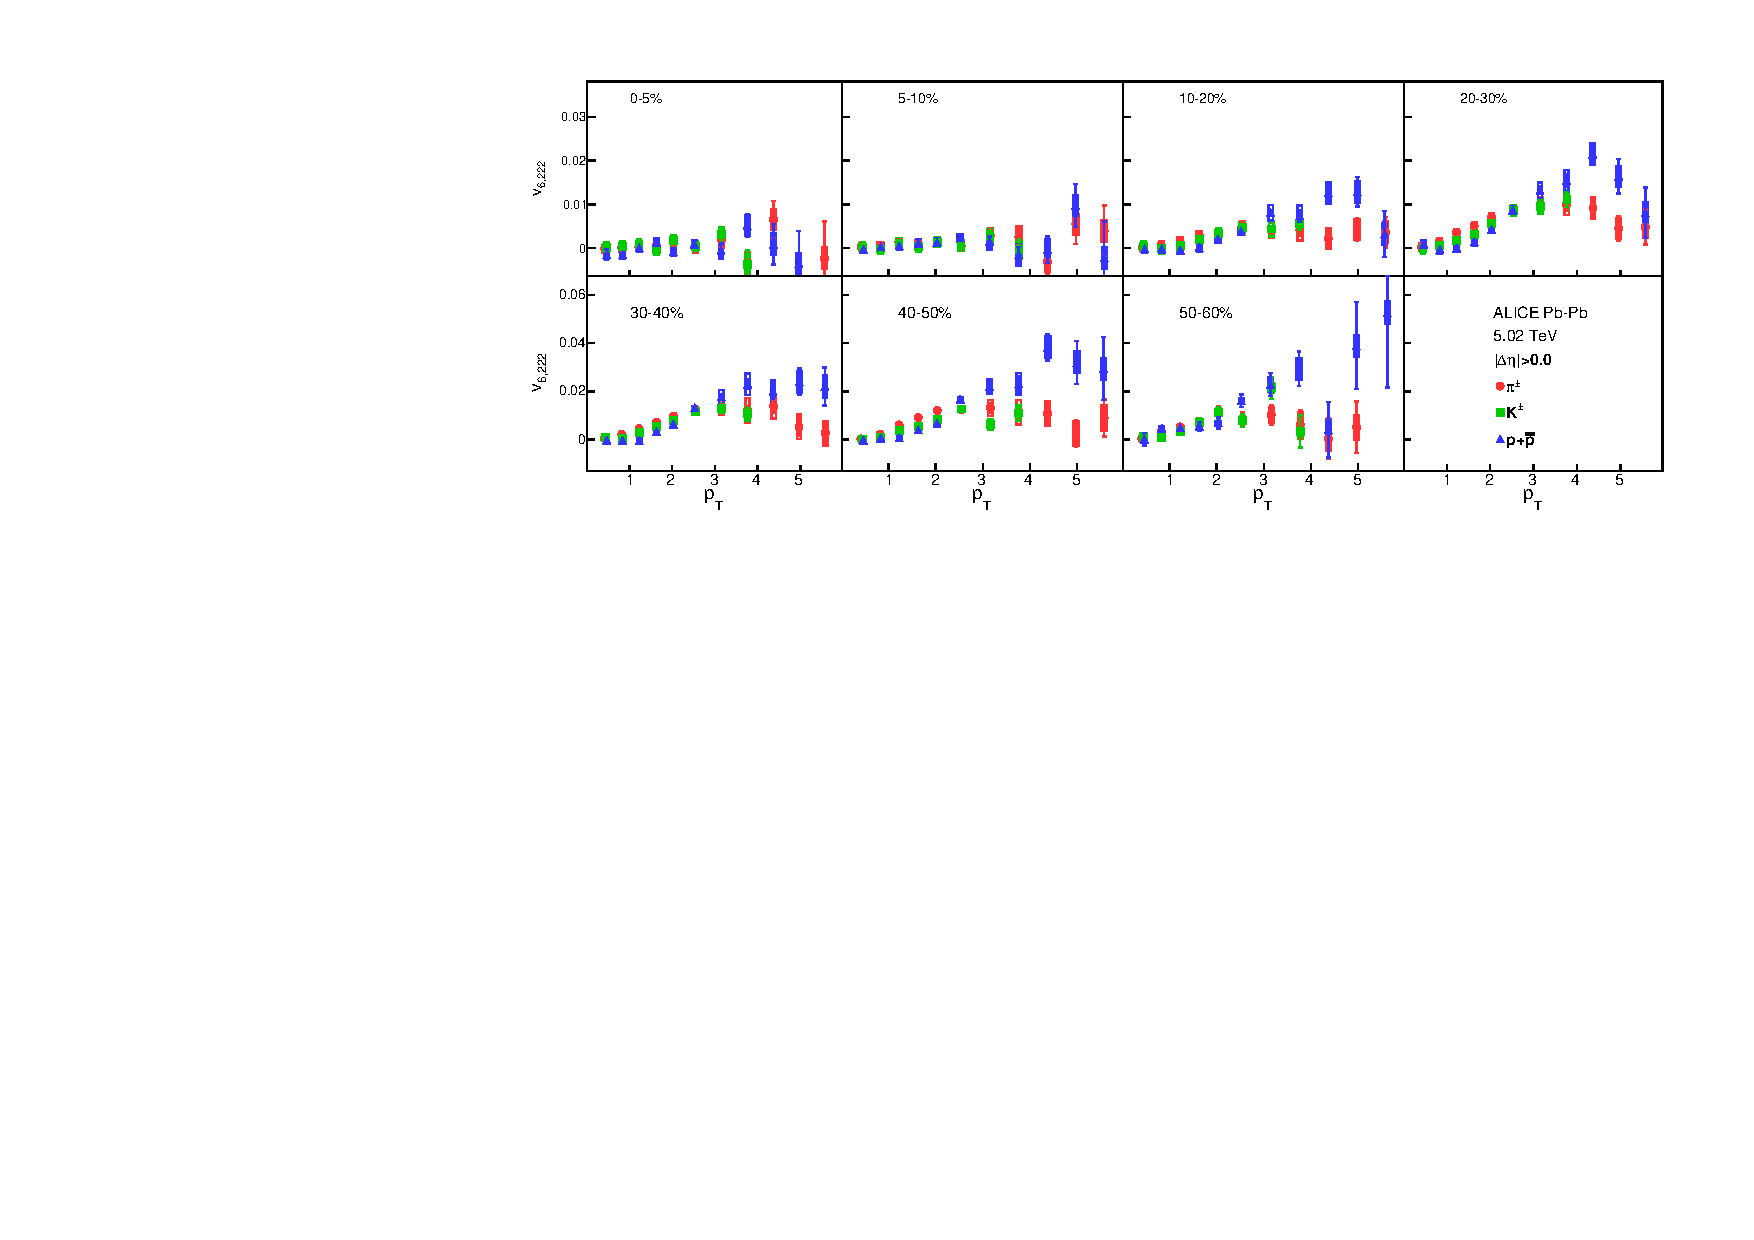
\includegraphics[scale=0.82]{figures/results/All_v6222_gap00.pdf}
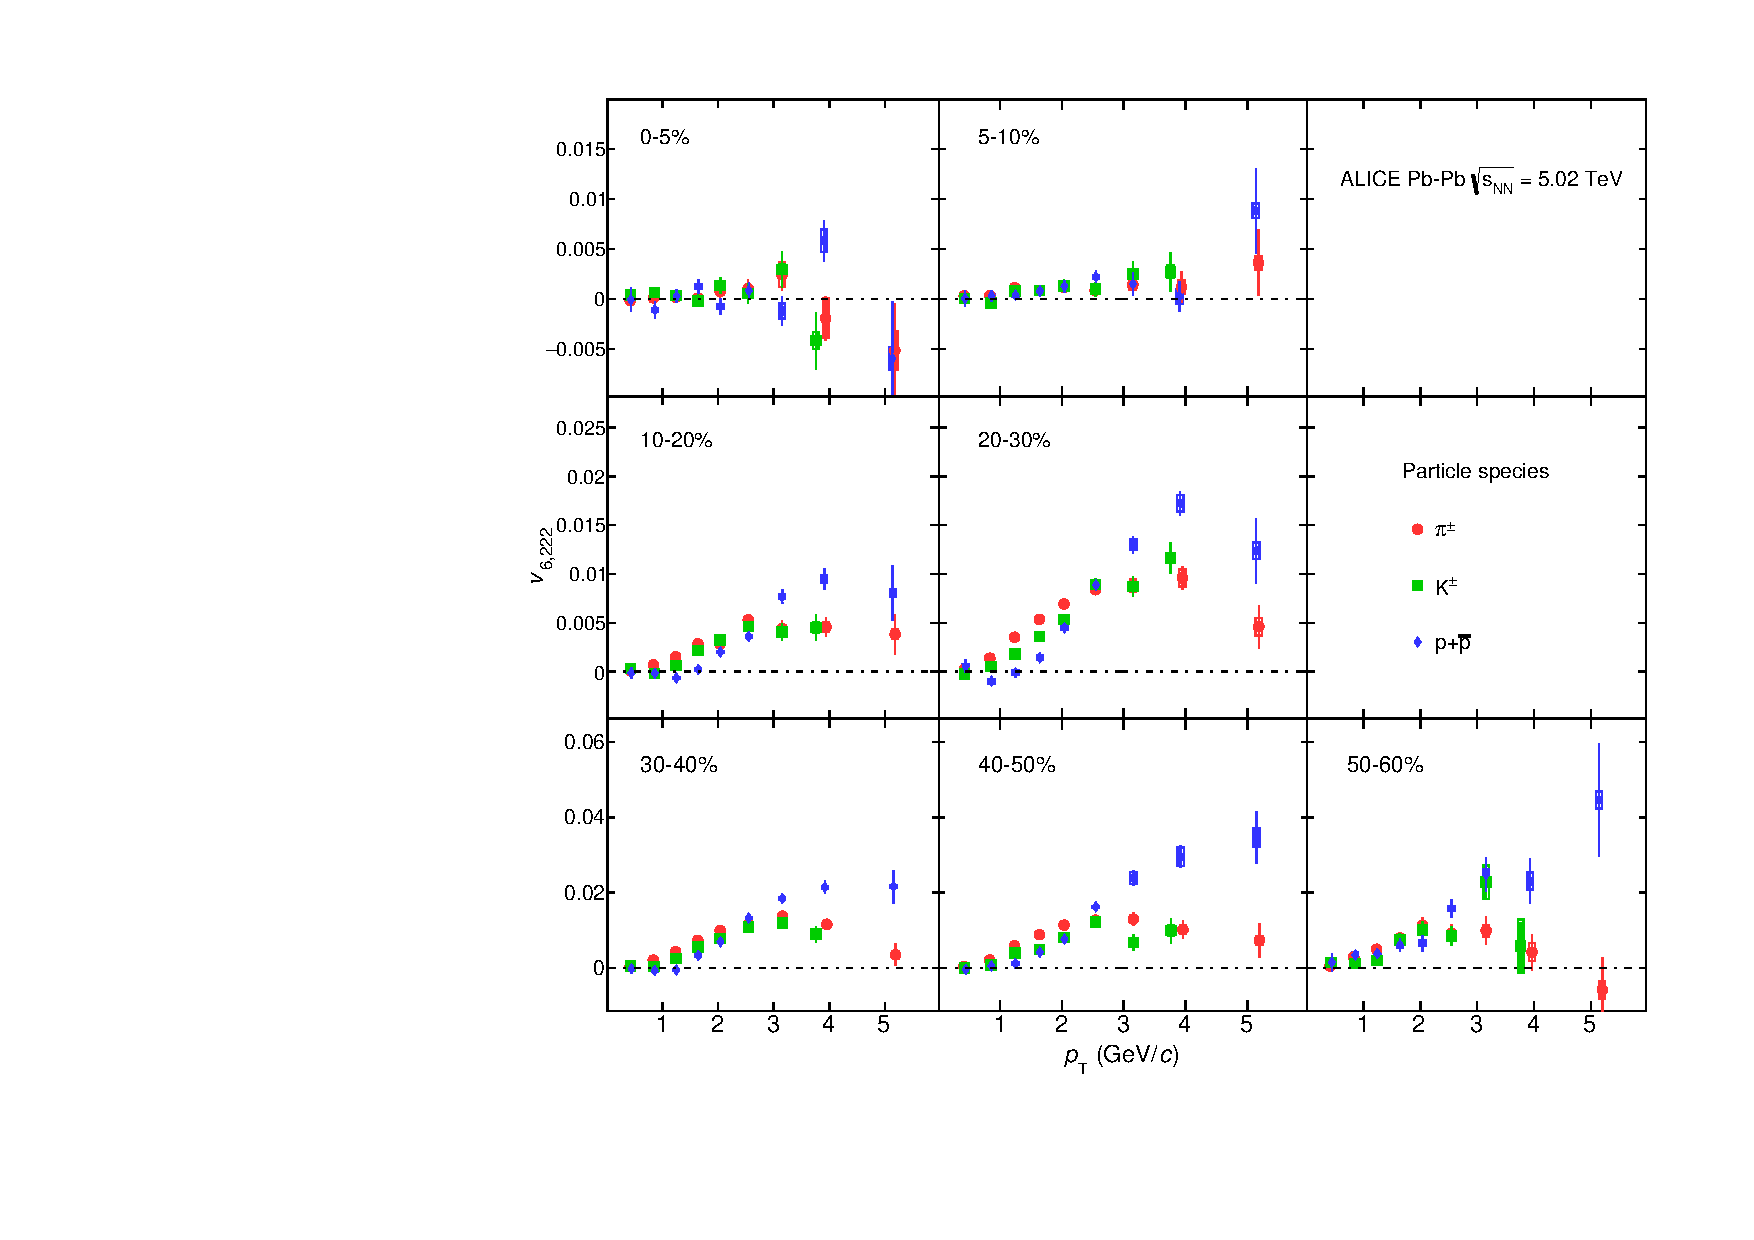
\includegraphics[scale=0.82]{figures/results/All_v6222_gap00_PID2_3by3.pdf}

\end{center}
\caption{The \pT-differential $v_{6,222}$ for different particle species grouped into different centrality intervals of Pb--Pb collisions at \sNN.}
\label{v6222_particleDependence}
\end{figure}

\newpage

In addition, in the intermediate \pT~region (for \pT $> 2.5$ \GeV) the data points of Figs. \ref{v422_particleDependence}-\ref{v6222_particleDependence} exhibit a particle type grouping. In particular, the data points form two groups, one for mesons and one for baryons with the values of $v_{n,mk}$ of the latter being larger. This particle type grouping was previously observed in $v_{n}$ measurements of various particle species \cite{Abelev:2014pua,Adam:2016nfo,Acharya:2018zuq,Adams:2003am,Abelev:2007qg,Adler:2003kt,Adare:2006ti}. 
This grouping was explained in Ref. \cite{Molnar:2003ff} in the picture of particle production via quark coalescence indicating that flow develops at the partonic stage. In this picture, known as NCQ scaling, the flow of mesons(baryons) are roughly twice(thrice) the flow of their constituent quarks in the intermediate transverse momentum region \cite{Voloshin:2002wa,Molnar:2003ff}. ALICE measurements have shown that this scaling at the LHC energies holds at an approximate level of 20\% for $v_{n}$ \cite{Abelev:2014pua,Adam:2016nfo,Acharya:2018zuq}. %Various theoretical ideas were created to address the origin of possible scaling by requiring quark coalescence to be the dominant particle production mechanism in the intermediate \pT~region, where the hydrodynamic evolution of the fireball is not the driving force behind the development of anisotropic flow \cite{Voloshin:2002wa,Molnar:2003ff}.

%This suggests that flow develops at the partonic stage and if so, combining two or three quarks to form hadronic states might result into hadrons inheriting the transverse momentum and subsequently, $v_{n}$ of their constituents. As a next step it was suggested in \cite{Molnar:2003ff} to use a form of number of constituent quark (NCQ) scaling in which both flow coefficients and \pT~were scaled by the number of constituent quarks ($n_{q}$). This worked initially at RHIC energies, although later measurements revealed sizeable deviations from a perfect scaling \cite{Adams:2003am,Abelev:2007qg,Adler:2003kt,Adare:2006ti}. ALICE measurements showed that the NCQ scaling at LHC energies holds at an approximate level of 20\% for $v_{n}$ \cite{Abelev:2014pua,Adam:2016nfo,Acharya:2018zuq}. Various theoretical ideas were created to address the origin of possible scaling by requiring quark coalescence to be the dominant particle production mechanism in the intermediate \pT~region, where the hydrodynamic evolution of the fireball is not the driving force behind the development of anisotropic flow \cite{Voloshin:2002wa,Molnar:2003ff}.

%\subsection{Test of scaling properties}
%\label{subsection:NCQscaling}

Figures \ref{v422_NCQ}, \ref{v523_NCQ}, \ref{v633_NCQ} and \ref{v6222_NCQ} present $v_{4,22}$, $v_{5,32}$, $v_{6,33}$ and $v_{6,222}$ respectively, scaled by the number of constituent quarks ($n_{q}$) as a function of \pTnq~for \pion, \kaon, \Ks, \proton, \lambdas~and $\phi$-meson grouped in different centrality intervals. The scaling is consistent with the observations reported for higher order anisotropic flow coefficients \cite{Acharya:2018zuq}. It is seen that for the non-linear flow modes this scaling holds at an approximate level ($\pm$20\%) for \pT $> 1$ \GeVc,~where quark coalescence is expected to be the dominant process.

\begin{figure}[!htb]
\begin{center}
%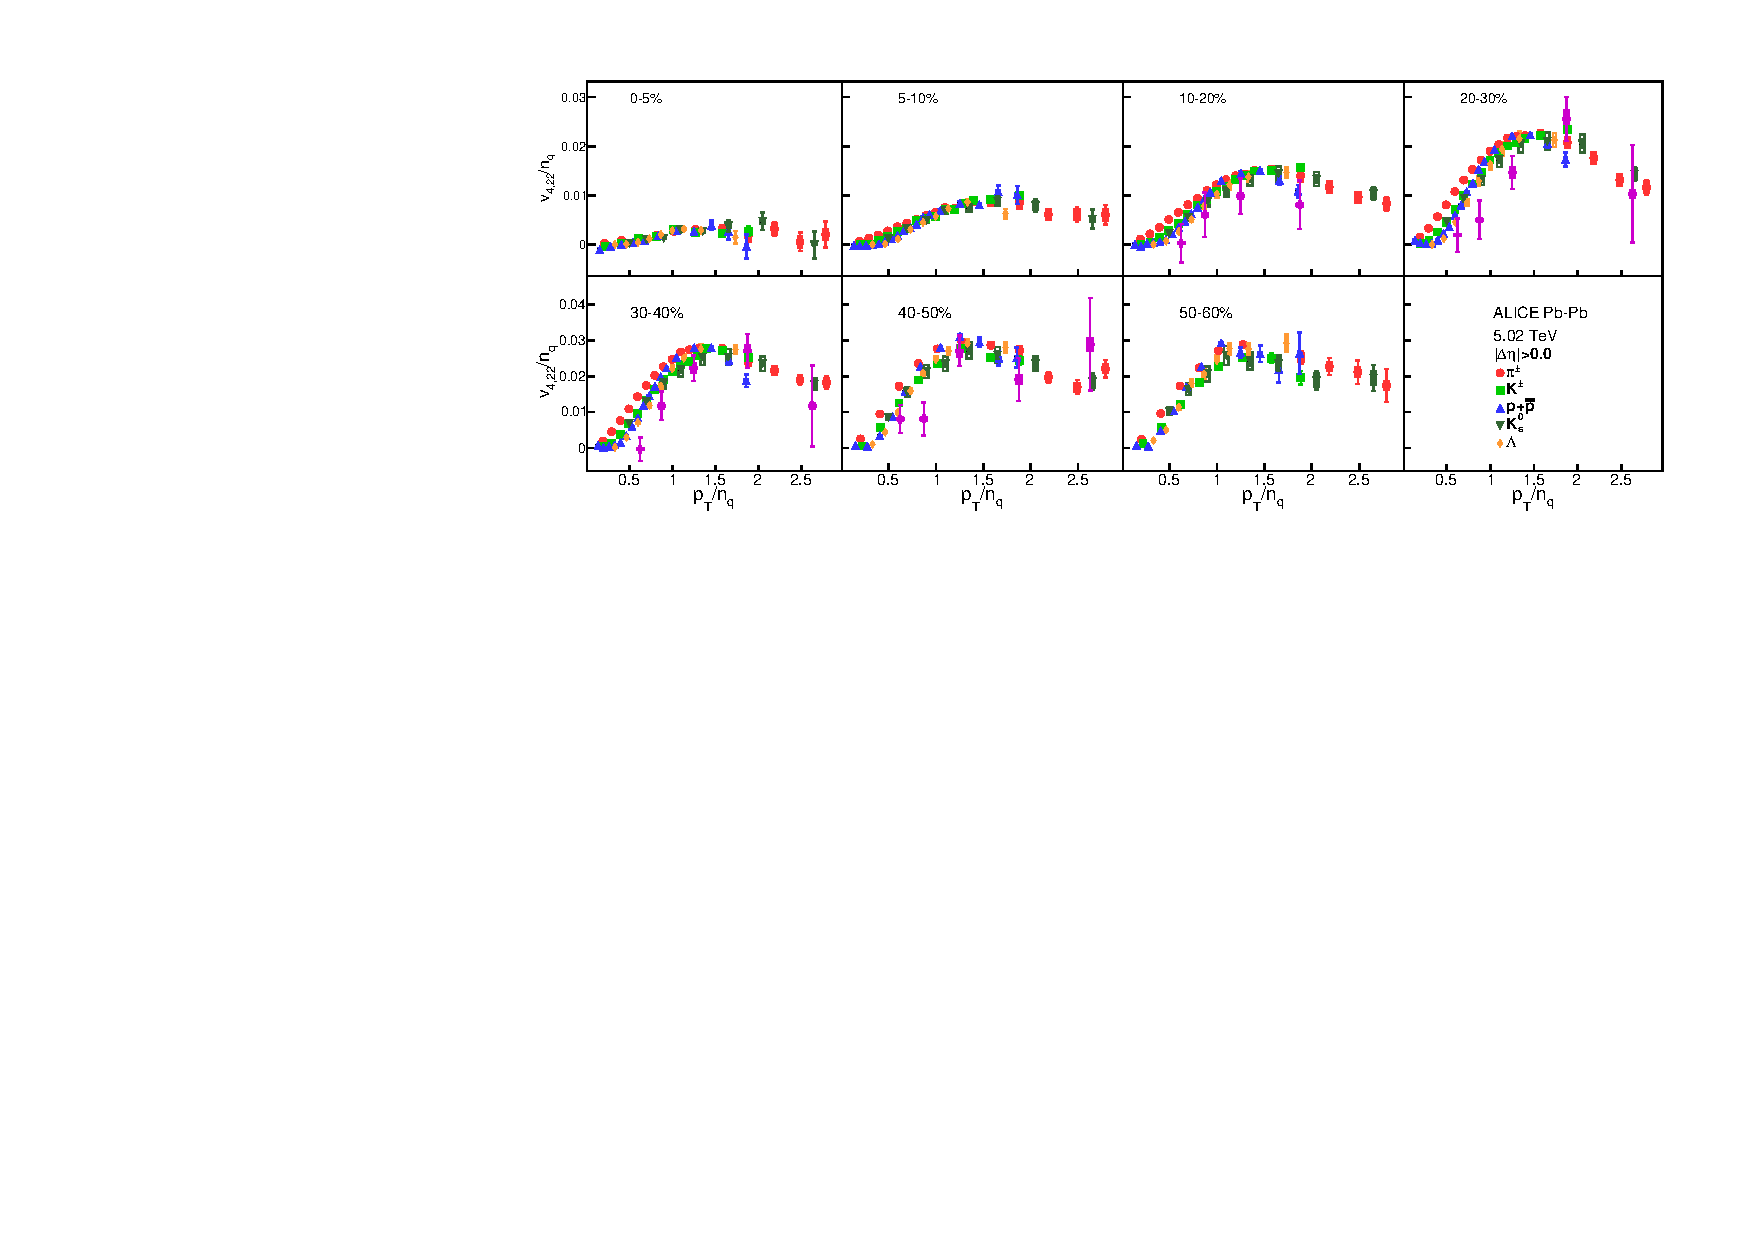
\includegraphics[scale=0.82]{figures/scaling/All_v422_gap00_NCQ.pdf}
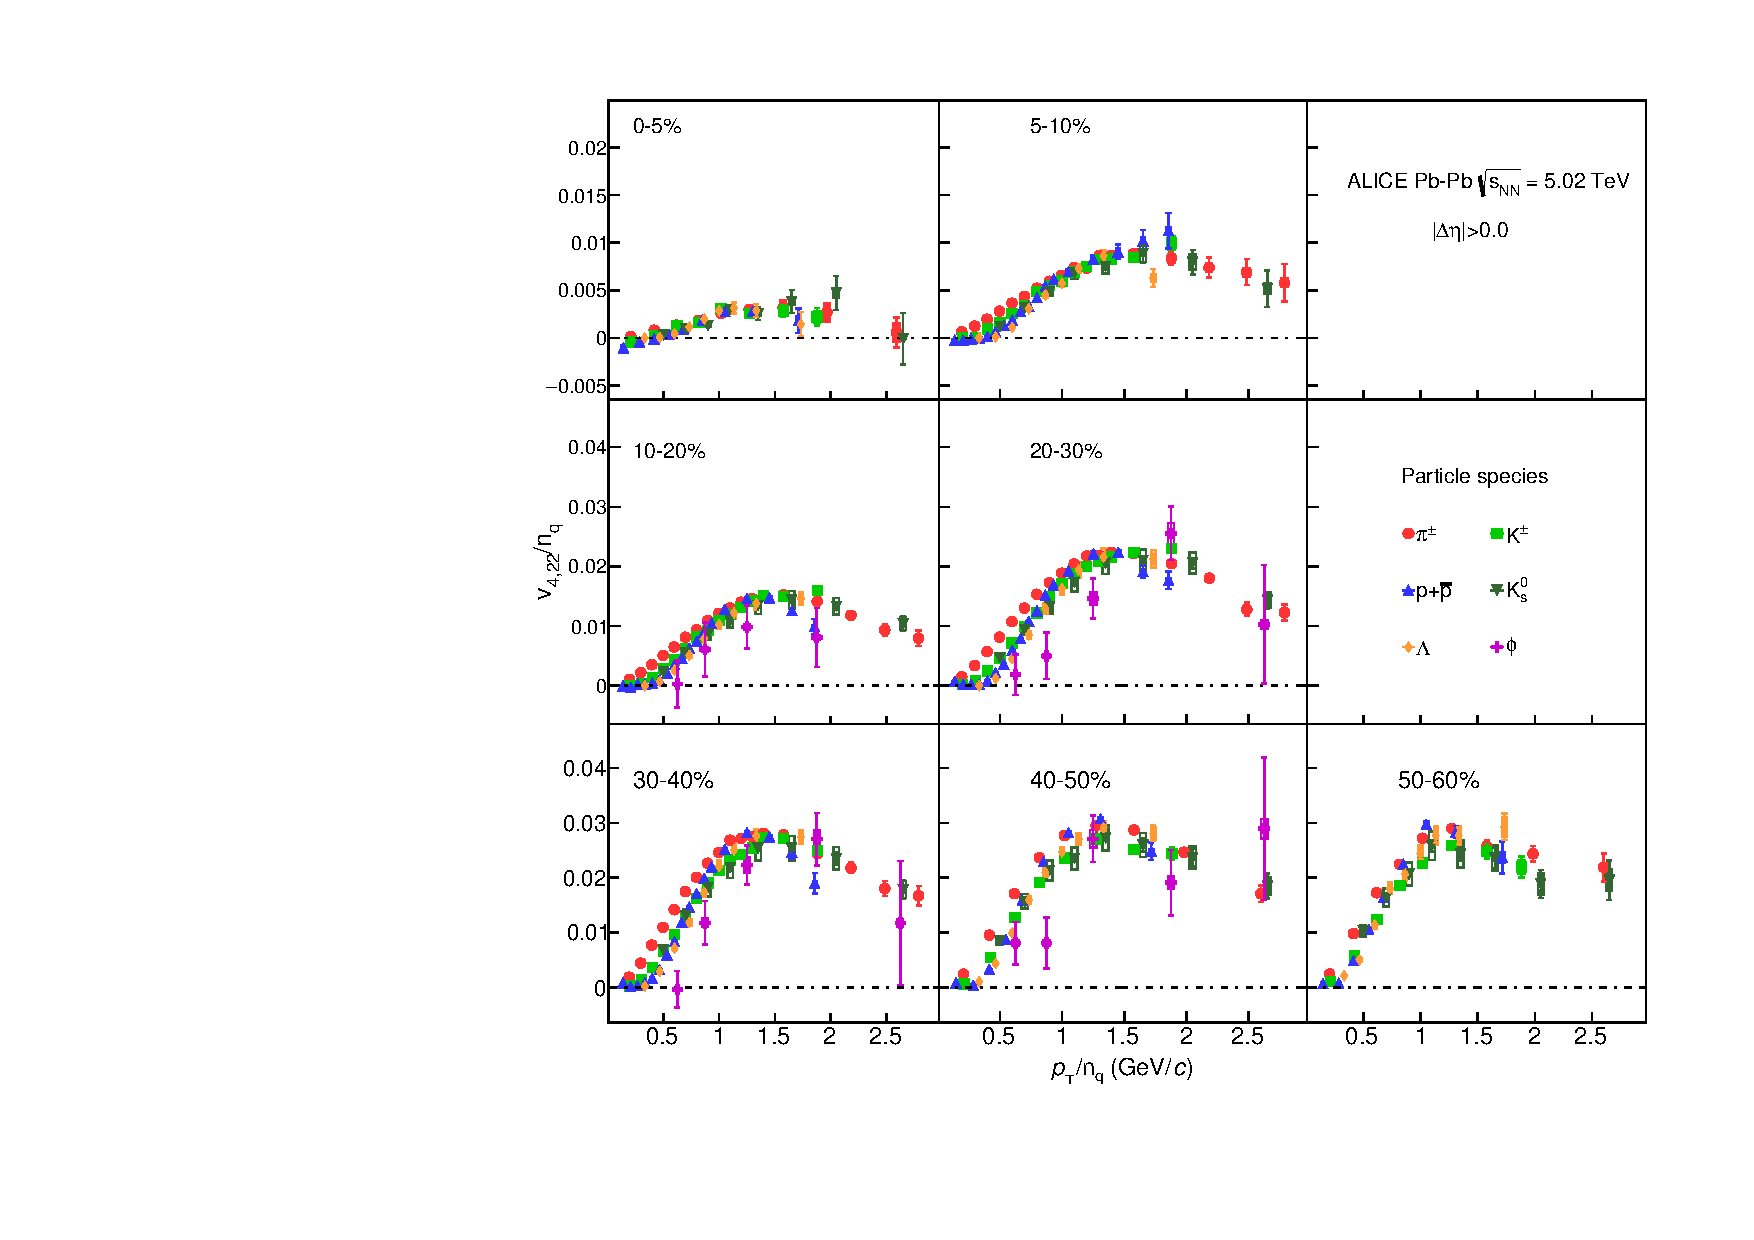
\includegraphics[scale=0.82]{figures/scaling/All_v422_gap00_NCQ_3by3.pdf}
\end{center}
\caption{The $p_{\rm{T}}/n_{q}$-dependence of $v_{4,22}/n_{q}$ for different particle species grouped into different centrality intervals of Pb--Pb collisions at \sNN.}
\label{v422_NCQ}
\end{figure}

\begin{figure}[!htb]
\begin{center}
%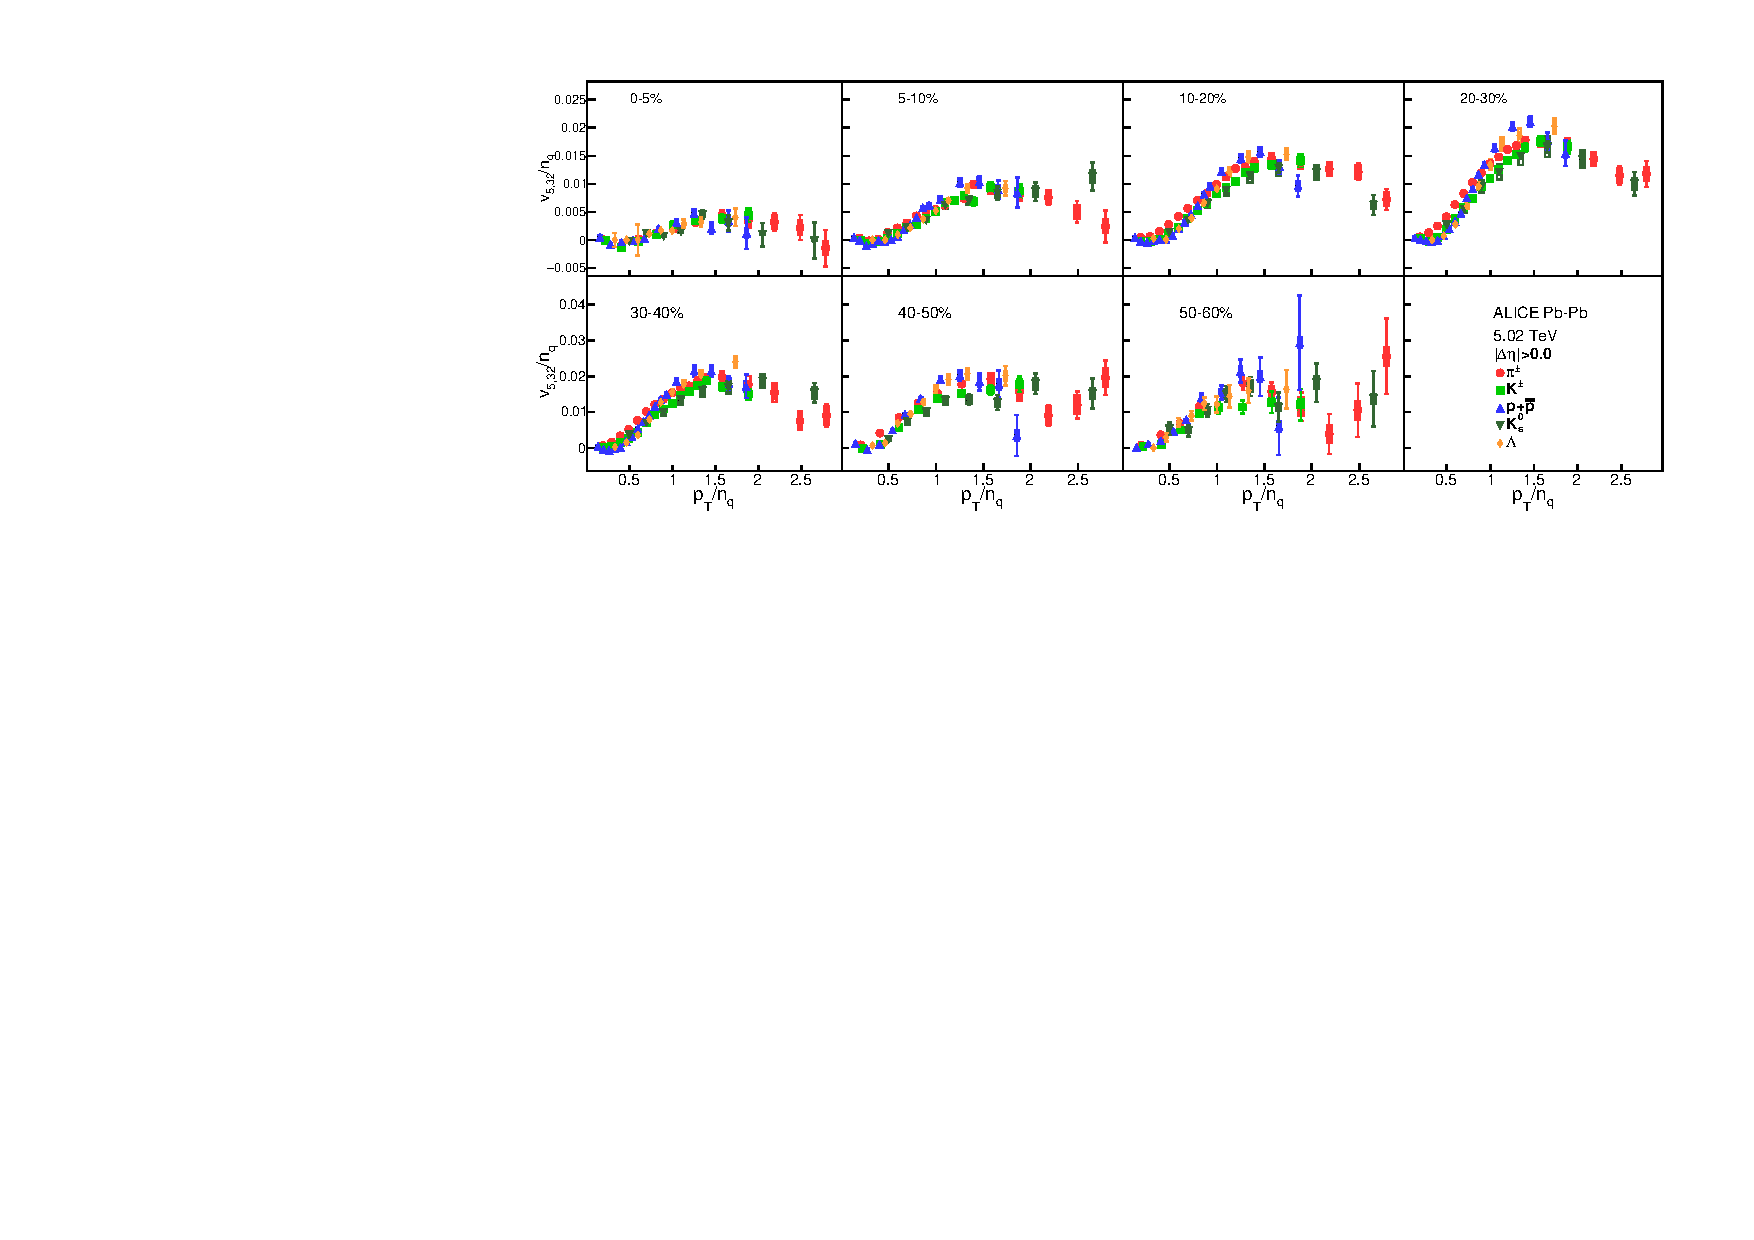
\includegraphics[scale=0.82]{figures/scaling/All_v523_gap00_NCQ.pdf}
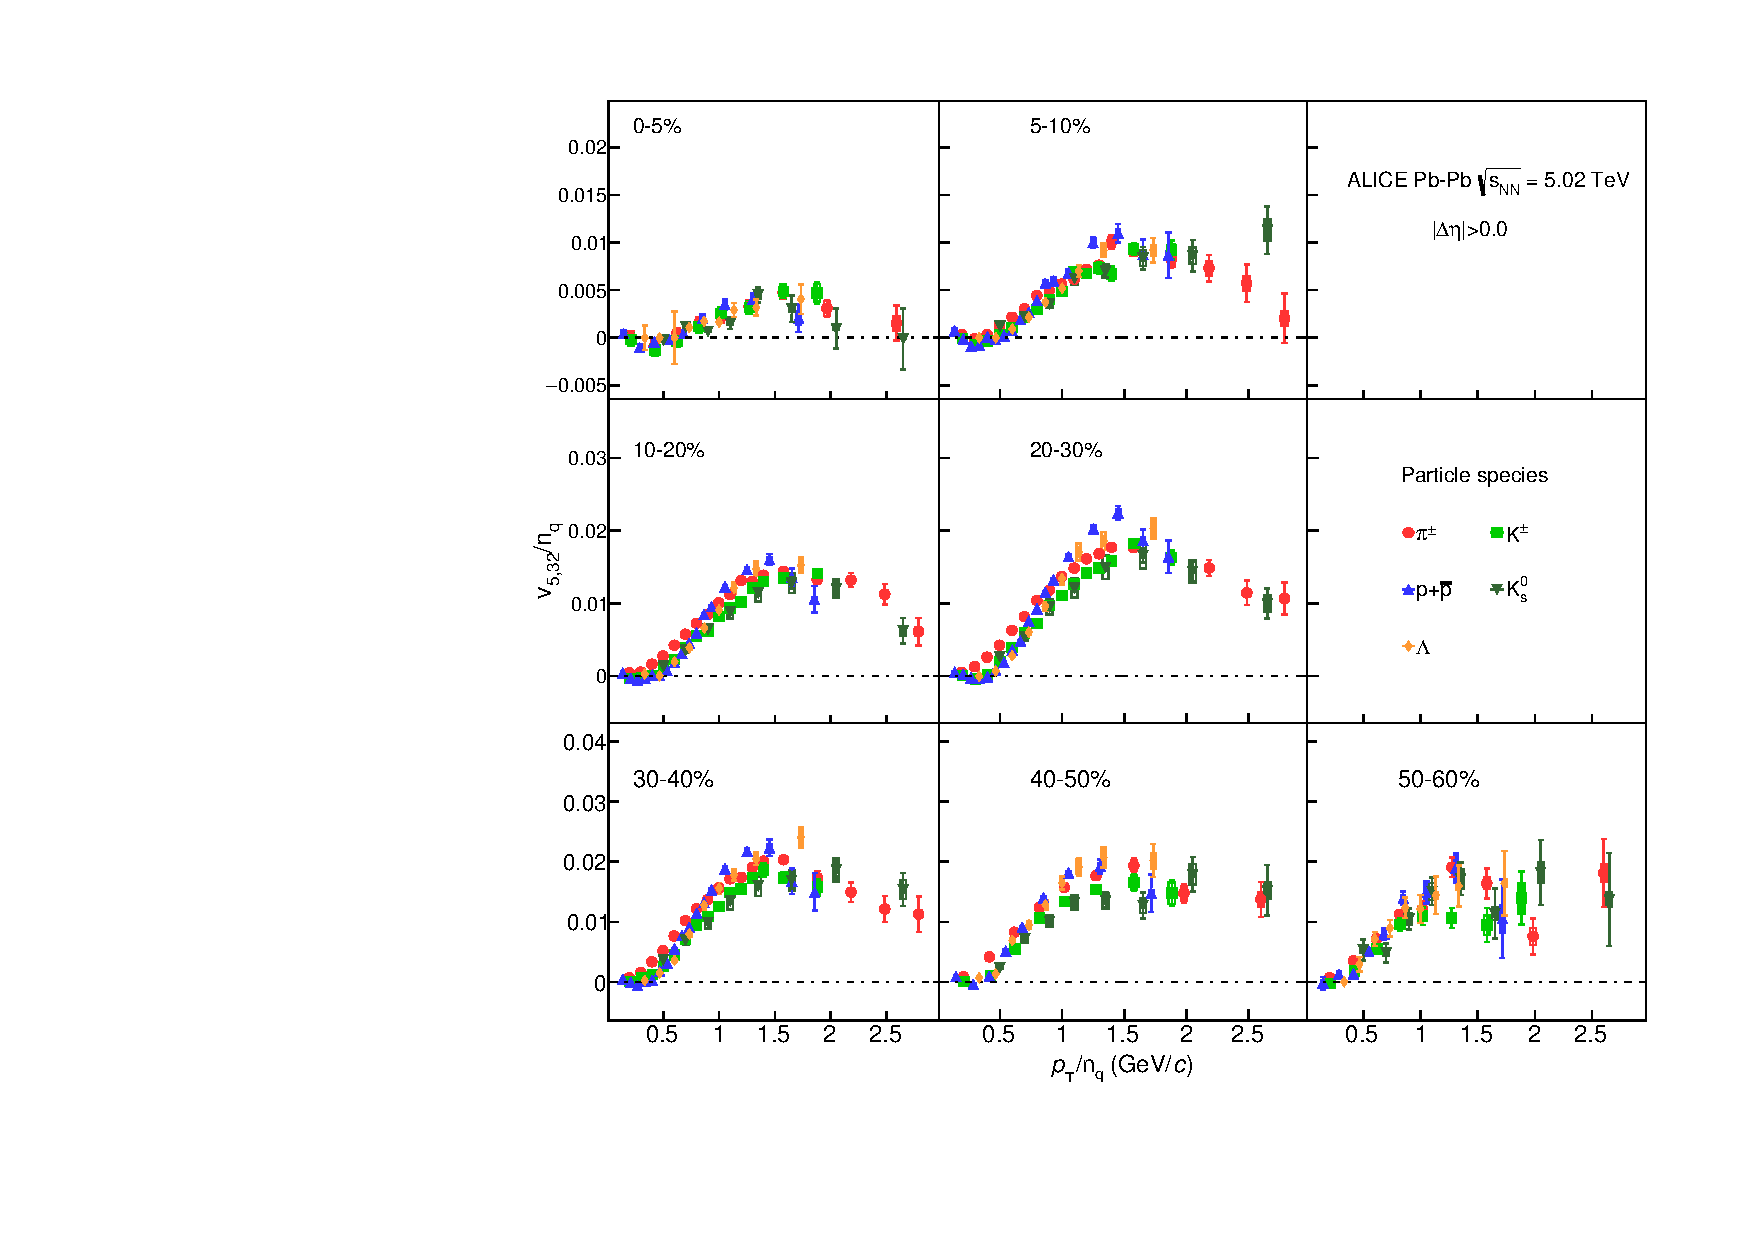
\includegraphics[scale=0.82]{figures/scaling/All_v523_gap00_NCQ_3by3.pdf}

\end{center}
\caption{The $p_{\rm{T}}/n_{q}$-dependence of $v_{5,32}/n_{q}$ for different particle species grouped into different centrality intervals of Pb--Pb collisions at \sNN.}
\label{v523_NCQ}
\end{figure}

\begin{figure}[!htb]
\begin{center}
%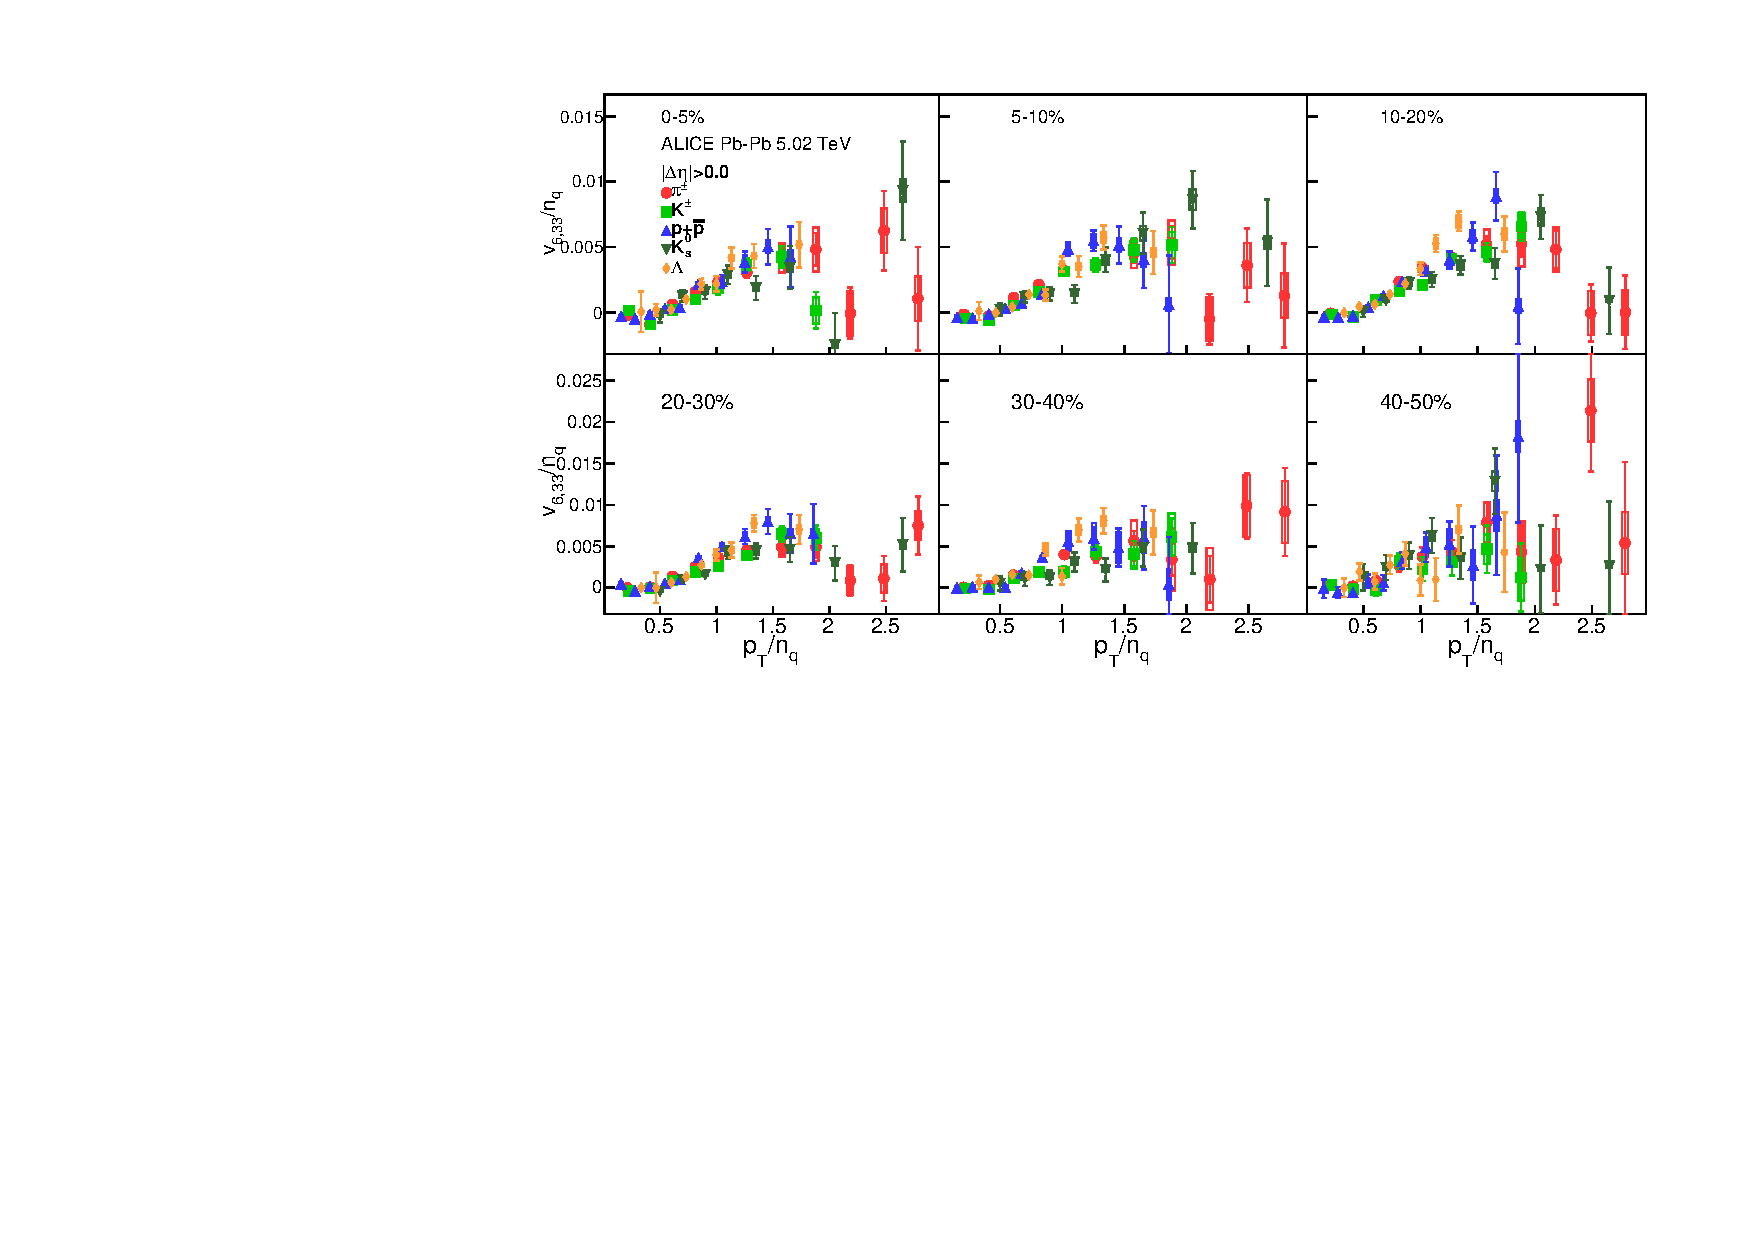
\includegraphics[scale=0.82]{figures/scaling/All_v633_gap00_NCQ.pdf}
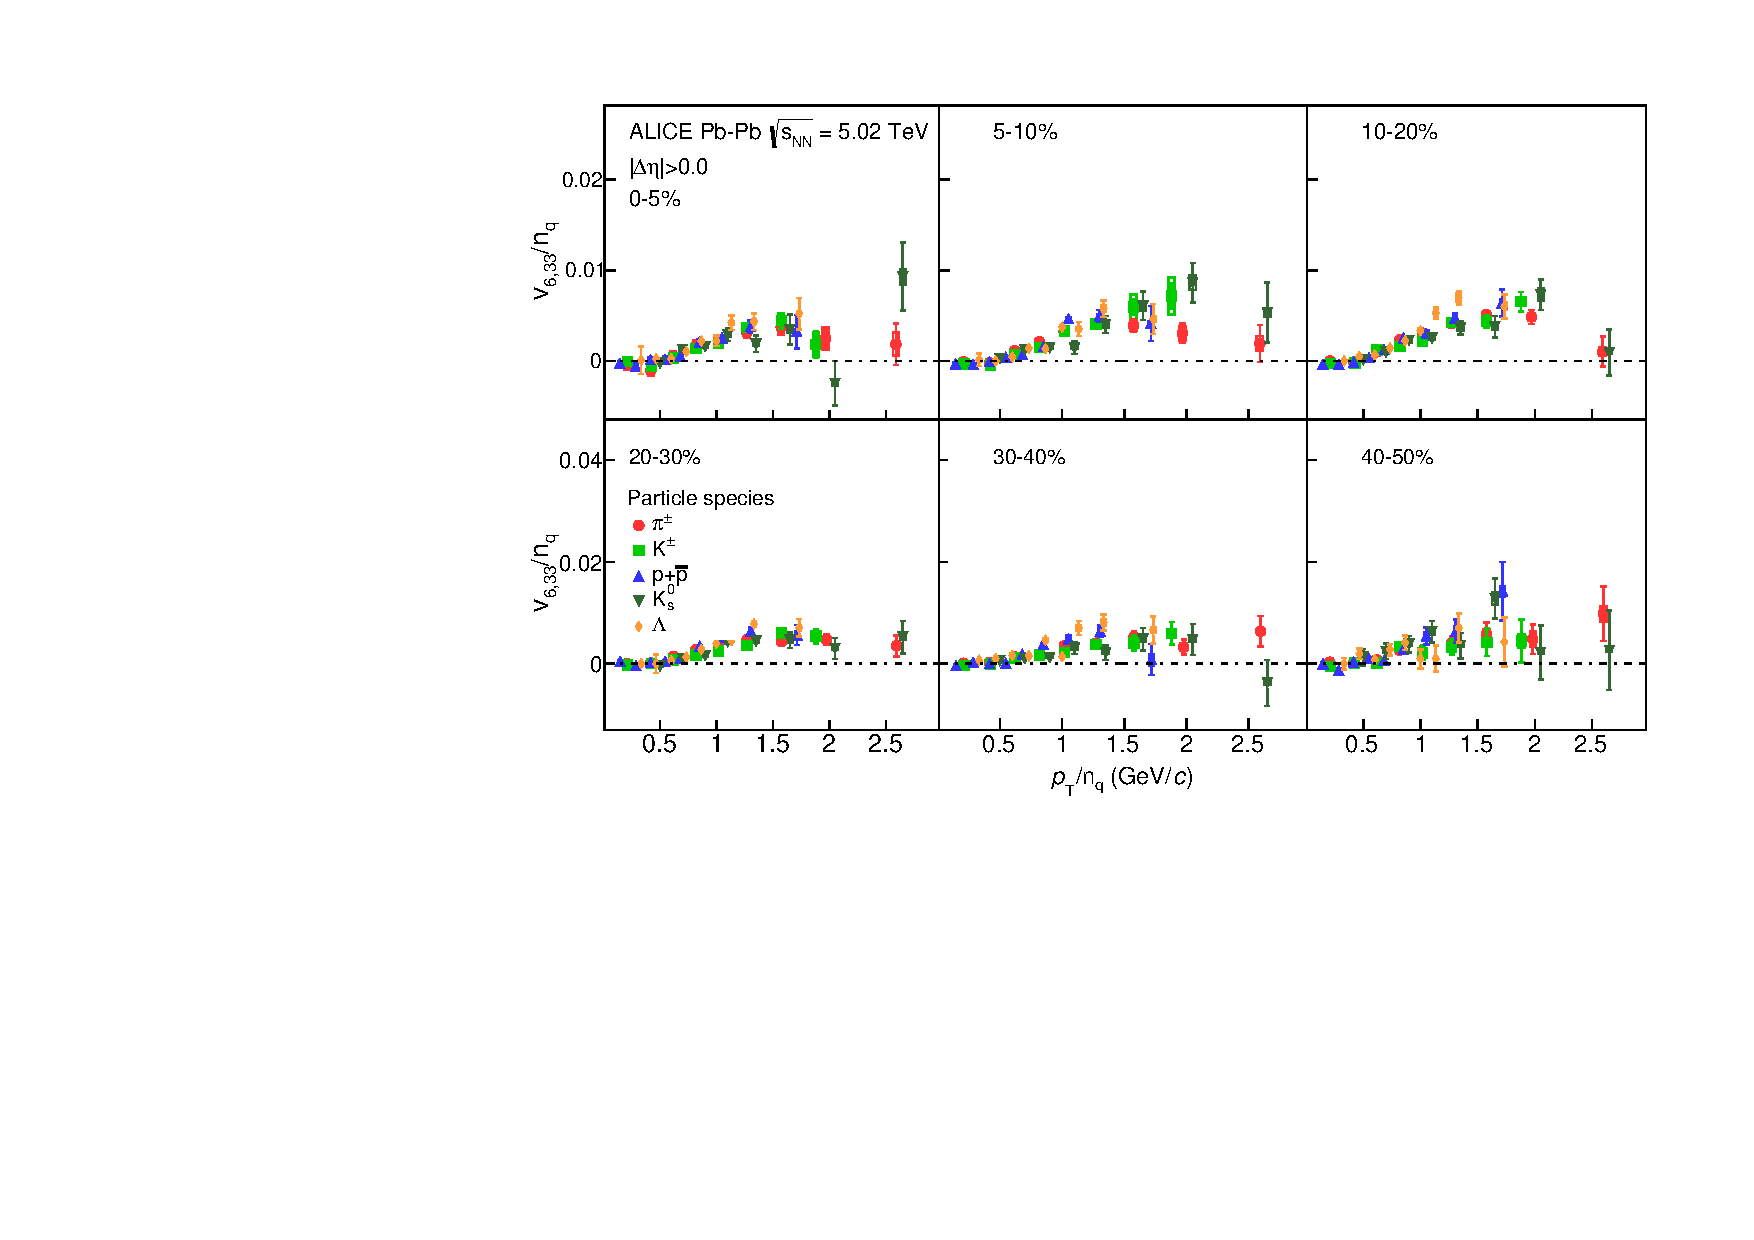
\includegraphics[scale=0.82]{figures/scaling/All_v633_gap00_NCQ_3by2.pdf}
\end{center}
\caption{The $p_{\rm{T}}/n_{q}$-dependence of $v_{6,33}/n_{q}$ for different particle species grouped into different centrality intervals of Pb--Pb collisions at \sNN.}
\label{v633_NCQ}
\end{figure}

\begin{figure}[!htb]
\begin{center}
%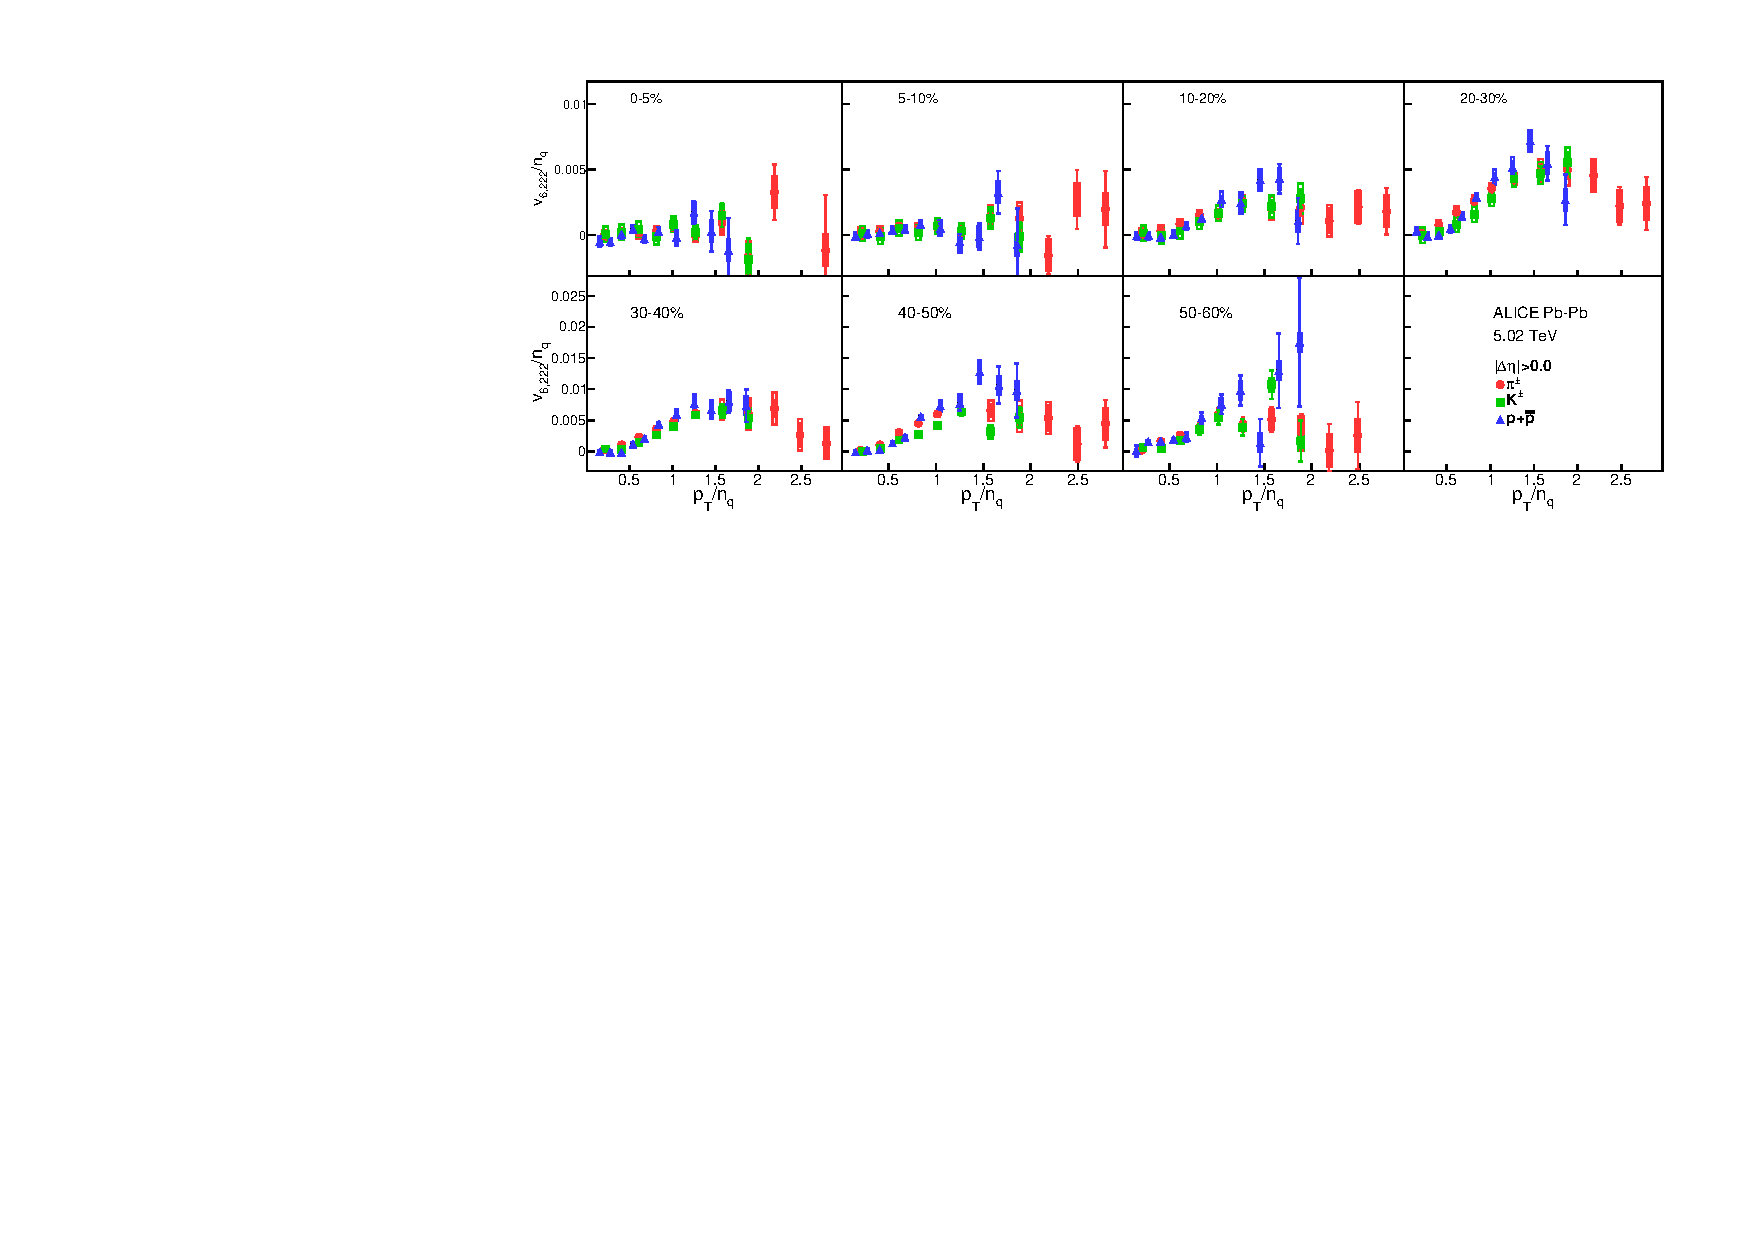
\includegraphics[scale=0.82]{figures/scaling/All_v6222_gap00_NCQ.pdf}
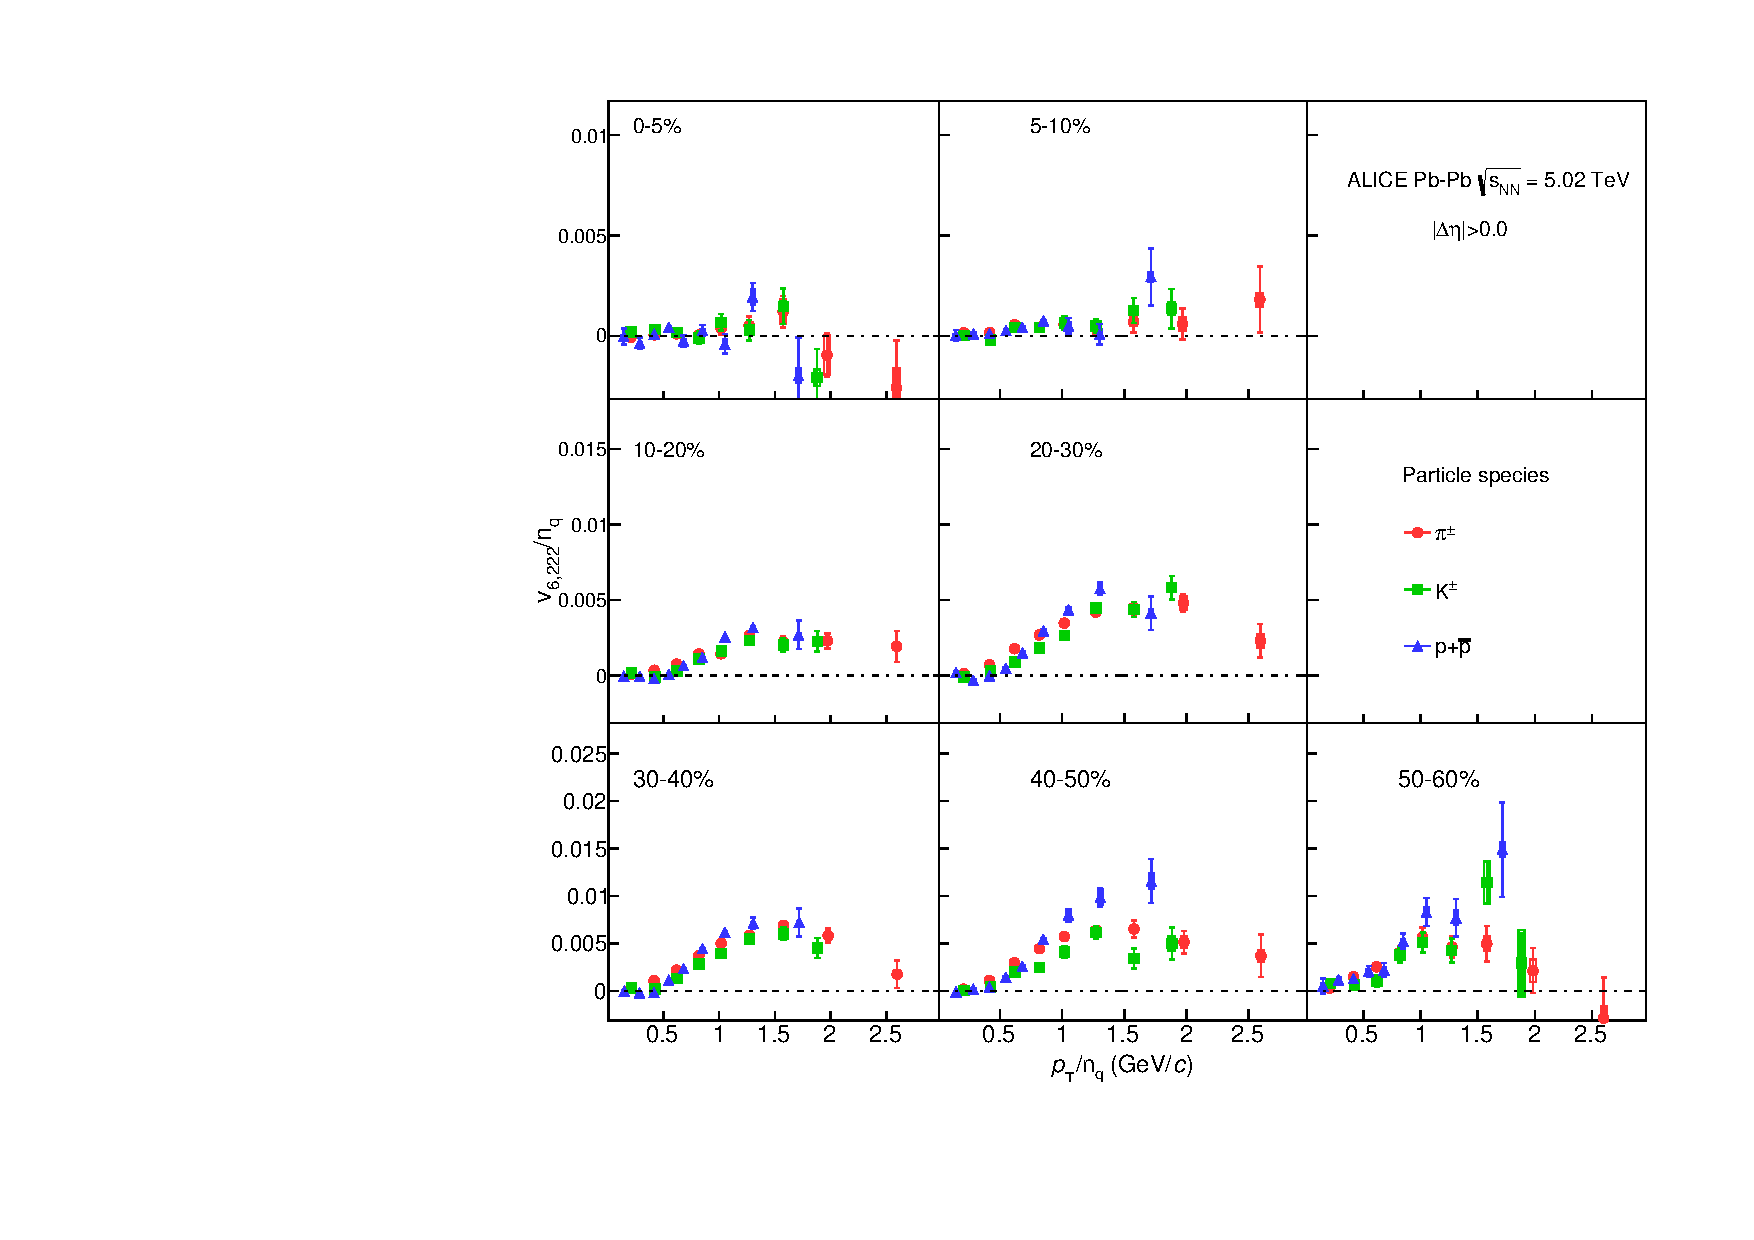
\includegraphics[scale=0.82]{figures/scaling/All_v6222_gap00_NCQ_3by3.pdf}

\end{center}
\caption{The $p_{\rm{T}}/n_{q}$-dependence of $v_{6,222}/n_{q}$ for different particle species grouped into different centrality intervals of Pb--Pb collisions at \sNN.}
\label{v6222_NCQ}
\end{figure}


\subsection{Comparison with $v_{n}$ of identified particles}
\label{SubSec:comparewithvn}

%The features seen in the measurement of non-linear flow modes can be further studied by comparing to that of anisotropic flow coefficients. 
The comparison of the features discussed before i.e. mass ordering and particle type grouping between the non-linear and the anisotropic flow coefficient is of particular interest.  Based on a naive expectation the mass ordering should develop quantitatively in a different way between the non-linear (i.e. due to the dependence on $\varepsilon_{2}^{2}$) and the anisotropic flow coefficient. In parallel, if coalescence is the dominant particle production mechanism in the intermediate \pT~region, one expects a similar grouping between $v_{n}^{\rm NL}$ and $v_{n}$. Such comparison could only be performed for $v_{4,22}$(\pT) (this study) and $v_{4}$(\pT) measurements \cite{Acharya:2018zuq} and was done by taking the difference between pions and protons at a given \pT~in both modes and normalising it by the integrated flow of the corresponding mode for charged particles \cite{Adam:2016izf} ($[v_{4}^{\pi^{\pm}} -  v_{4}^{\rm p+\bar{p}}](p_{\rm T}) / v_{4}^{\rm h^{\pm}}$). This comparison is shown in Fig. \ref{massOrderingComparison} for 0-5\% up to 40-50\% centrality interval. It can be seen that in the low \pT~region (\pT~< $2.5-3$ \GeV) where the mass ordering is prominent, the data points exhibit a general agreement for all centrality intervals. However, there is a hint that the relative ratio for $v_{4,22}$ is smaller than the one of the $v_{4}$ for \pT~$< 0.8$ \GeV~and for centrality ranges 0-30\%.
%the comparison shows two features. At very low \pT~values~(\pT~< $0.8$ \GeV), the ratio for $v_{4}$ shows slightly lower magnitude with respect to that of $v_{4,22}$ from 0-5\% up to 20-30\% centrality intervals. At more peripheral collisions, the ratios are compatible. 
If this difference and its centrality dependence persists for lower values of \pT, it could indicate that the hydrodynamic evolution is reflected differently in $v_{4}$ and $v_{4,22}$ and could be explained by the contribution of $\varepsilon_{2}^{2}$.  As it was stated earlier, the mass splitting is a result of an interplay of radial and anisotropic flow, leading to a stronger in-plane expansion compared to out-of-plane, and the particle thermal motion. Particle of a larger mass have smaller thermal velocities, and are affected stronger by the difference between in- an out-of-plane expansion velocities, thus leading to the mass splitting of $v_{n}$(\pT). The comparison of the \pT~dependence of $v_{n}^{\rm NL}$ and $v_{n}$ can provide a unique opportunity to test this picture, as it would allow to compare the results for the cases of exactly the same average radial flow and temperature, but differing by the anisotropic flow. On the other hand, in the intermediate \pT~region (\pT~> 2.5 \GeV), the same comparison shows that the results are compatible in all centrality intervals within one standard deviation. This implies a similar particle type grouping between $v_{4}$ and $v_{4,22}$ which is in line with the expectation that quark coalescence affects both flow modes  similarly.
%indicating similar particle type grouping in $v_{4}$ and $v_{4,22}$. This observation suggests that quark coalescence affects both flow modes  similarly.
%By increasing the \pT~value ($0.8$ <~\pT~< $2.5-3$ \GeV), this difference disappears which points to a similar mass ordering between $v_{4}$ and $v_{4,22}$ at this \pT~region.
%This comparison shows that the observed mass ordering in low \pT~region ($1$ <~\pT~< $2.5$ \GeV) is of the same magnitude in $v_{4,22}$ and $v_{4}$, however, for \pT~< $1$ \GeV, the mass ordering $v_{4}$ drops more rapidly compared to that of $v_{4,22}$.
%In the intermediate \pT~region (\pT~> 2.5 \GeV), the same comparison shows that the results are compatible in all centrality intervals within $1\sigma$. If this ratio could account for particle type grouping, similar particle type grouping in $v_{4,22}$ and $v_{4}$ measurements. 


\begin{figure}[!htb]
\begin{center}
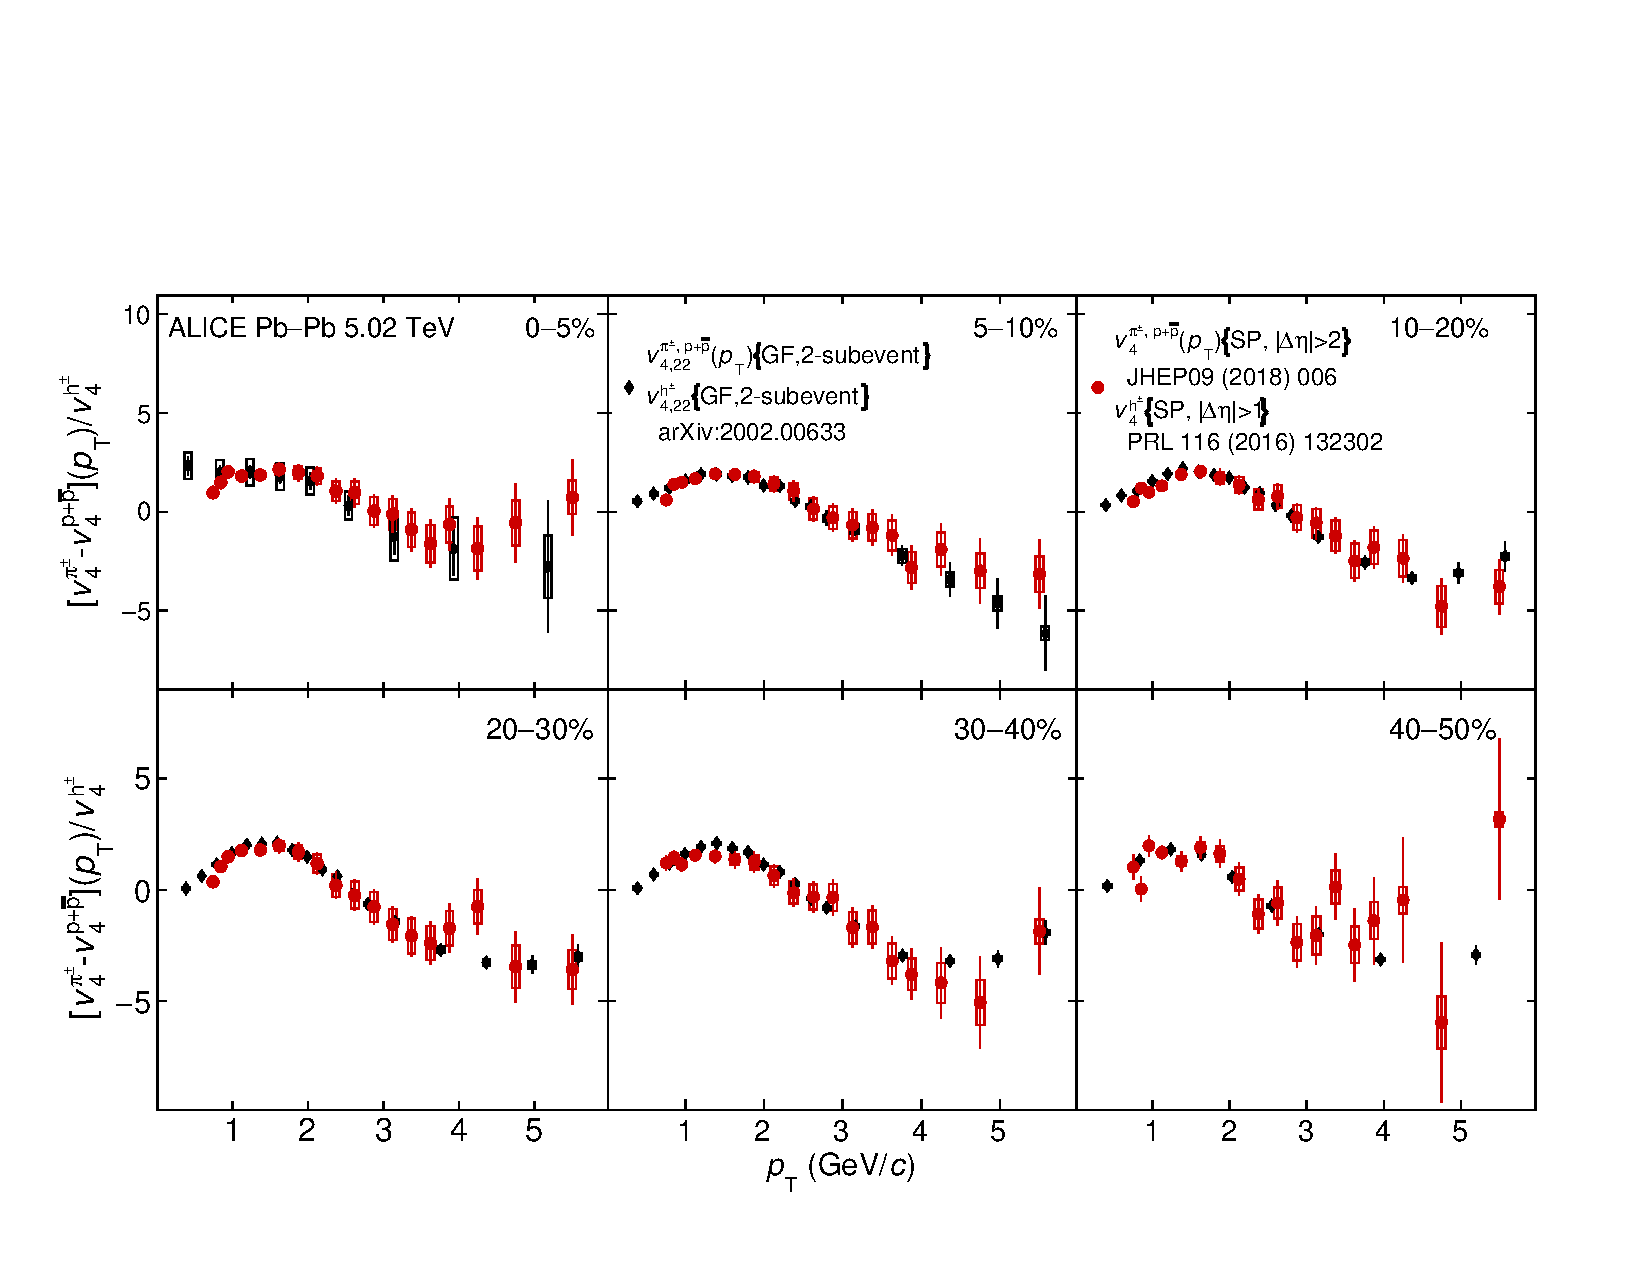
\includegraphics[scale=0.6]{figures/results/massOrdering_vn_pion_proton_to_charged.pdf}
\end{center}
\caption{The comparison between $[v_{4,22}^{\pi^{\pm}} -  v_{4,22}^{\rm p+\bar{p}}](p_{\rm T}) / v_{4,22}^{\rm h^{\pm}} $ and $[v_{4}^{\pi^{\pm}} -  v_{4}^{\rm p+\bar{p}}](p_{\rm T}) / v_{4}^{\rm h^{\pm}} $  grouped into different centrality intervals of Pb--Pb collisions at \sNN.}
\label{massOrderingComparison}
\end{figure}


%$\frac{\Delta v_{4,22}^{\pi^{\pm}}-v_{4,22}^{p+\bar{p}}$(p_{rm T})}{v_{4,22}^{h^{\pm}}}$

\newpage
\subsection{Comparison with models}
\label{SubSec:hydro}
%Measurements of anisotropic flow coefficients, $v_{n}$, at RHIC and the LHC are described well by hydrodynamic calculations \cite{Xu:2016hmp, McDonald:2016vlt, Zhao:2017yhj}. 

The comparison of various anisotropic flow measurements and hydrodynamic calculations have been presented and discussed in great details in \cite{Xu:2016hmp, McDonald:2016vlt, Zhao:2017yhj}. A recent comparison between $v_{n}$ measurements reported by ALICE \cite{Acharya:2018zuq} and two hydrodynamic calculations from \cite{Zhao:2017yhj} shed new light on the initial conditions and the transport properties of the created system in Pb--Pb collisions. Both hydrodynamic calculations are based on iEBE-VISHNU \cite{Shen:2014vra}, an event-by-event version of the VISHNU hybrid model \cite{Song:2010aq} coupling $2+1$~dimensional viscous hydrodynamics (VISH2+1) \cite{Song:2007fn} to a hadronic cascade model (UrQMD). The initial conditions used for these calculations are described by AMPT \cite{Lin:2004en} and TRENTo \cite{Moreland:2014oya}, both with $\tau_{0}$=0.6 fm/$c$ and $T_{sw}$ =148 MeV \cite{Bernhard:2016tnd}. For AMPT initial conditions, constant values of specific shear viscosity ($\eta/s =0.08$, the lower limit conjectured by AdS/CFT) and bulk viscosity ($\zeta/s = 0$) are utilised. The version of the model that uses TRENTo \cite{Moreland:2014oya} initial conditions incorporates a temperature dependent specific shear and bulk viscosity extracted from the global bayesian analysis \cite{Bernhard:2016tnd}. \footnote{ For simplicity in the rest of this article the model with AMPT initial conditions, $\eta/s =0.08$ and $\zeta/s =0$ is referred to as AMPT and the model with TRENTo initial conditions, $\eta/s(\rm{T})$ and $\zeta/s(\rm{T})$ is referred to as TRENTo.} 

The comparison between $v_{n}$ measurements and these two hydrodynamic calculations illustrates a qualitative agreement. This agreement between the data and the models depends on the particle species, transverse momentum range and centrality percentile. Overall, the AMPT model reproduces these measurements more accurately than the TRENTo model \cite{Acharya:2018zuq}. In order to further investigate the performance of these two models in reproducing $v_{n}$ measurements, the relative ratios between each model and the measurements of \pion, \kaon~and \proton~have been obtained. Table \ref{ModelDataComparisonflow} summarises these relative ratios. The values represent the ranges across all centralities that each model is able to describe the measurements of $v_n$ for each particle species. Comparison between the performance of the two models shows that the AMPT calculations reproduce $v_{2}$ slightly better that TRENTo. Both models reproduce the $v_{3}$ measurements relatively better than $v_{2}$, however AMPT performs better than TRENTo. Finally, the comparison between the models and $v_{4}$ measurements show that AMPT has an absolute better performance compared to TRENTo. These values should be taken with caution as $v_{4}$ has larger uncertainties with respect to $v_{3}$ and $v_{2}$. 

\begin{table}[!h]
\centering
\resizebox{0.81\textwidth}{!}{\begin{tabular}{ |p{4.5cm} |l|c|c|c|c|c|c|c|c|c|}
\hline
\multicolumn{1}{| c |}{} & \multicolumn{3}{| c |}{ $v_{2}$ } & \multicolumn{3}{| c |}{ $v_{3}$} & \multicolumn{3}{| c |}{ $v_{4}$}  \\
\hline
Error source  & \pion &  \kaon & \proton &  \pion & \kaon & \proton &  \pion &  \kaon & \proton \\ \hline  \hline
AMPT calculations & 3-13\% & 0-16\% & 0-20\% & 0-8\% & 5-12\% & 0-4\%& 6-12\% & 5-12\% & 0-4\%  \\
TRENTo calculations & 6-17\% & 0-19\% & 3-19\% & 2-15\% & 7-22\% & 0-11\% & 7-25\% & 16-28\% & 0-21\% \\
 \hline
\end{tabular}}

\caption{List of minimum and maximum value of the fit to relative ratios between the data and each model for  $v_{n} (n=2,3,4)$ of \pion, \kaon~and \proton. The minimum and maximum are obtained from 0-5\% up to 40-50\% centrality intervals .}\label{ModelDataComparisonflow}
\end{table}

\begin{table}[!h]
\resizebox{\textwidth}{!}{\begin{tabular}{ |p{4.5cm} |l|c|c|c|c|c|c|c|c|c|c|c|c|}
\hline
\multicolumn{1}{| c |}{} & \multicolumn{3}{| c |}{ $v_{4,22}$ } & \multicolumn{3}{| c |}{ $v_{5,32}$} & \multicolumn{3}{| c |}{ $v_{6,33}$} & \multicolumn{3}{| c |}{ $v_{6,222}$} \\
\hline
Error source  & \pion &  \kaon & \proton &  \pion & \kaon & \proton &  \pion &  \kaon & \proton &  \pion &  \kaon & \proton \\ \hline  \hline
AMPT claculations &  5-32\% & 2-30\%  & 3-30\% & 3-28\%  & 5-29\% &  1-65\% & 0-46\% & 0-46\% & 0-97\% & 6-52\% & 0-80\%  & 0-118\% \\
TRENTo calculations & 0-30\% & 4-33\% & 0-21\% &  24-49\% & 33-97\% & 12-58\% & 0-43\% & 0-46\% & 0-95\% & 0-20\% & 0-34\% & 0-78\%\\
 \hline
\end{tabular}}
\caption{List of minimum and maximum value of the fit to relative ratios between the data and each model for  $v_{n,mk}$ of \pion, \kaon~and \proton. The minimum and maximum are obtained from 0-10\% up to 50-60\% (40-50\% for $v_{6,33}$) centrality intervals .}\label{ModelDataComparisonNLflow}
\end{table}

%Recently, it was shown that the \pT-integrated non-linear flow modes are good observables to constrain the initial conditions and transport properties of the system \cite{Acharya:2017zfg}. 
%To test the validity of these hydrodynamic models a comparison is performed between the measured non-linear flow modes and two hydrodynamical calculations from \cite{Zhao:2017yhj}.  Both calculations are based on iEBE-VISHNU \cite{Shen:2014vra}, an event-by-event version of the VISHNU hybrid model \cite{Song:2010aq} coupling $2+1$~dimensional viscous hydrodynamics (VISH2+1) \cite{Song:2007fn} to a hadronic cascade model (UrQMD). One of these models uses AMPT \cite{Lin:2004en} initial conditions with constant values of specific shear viscosity ($\eta/s =0.08$, the lower limit conjectured by AdS/CFT) and bulk viscosity ($\zeta/s = 0$), and the other model incorporates TRENTo \cite{Moreland:2014oya} initial conditions with a temperature dependent specific shear and bulk viscosity. Both calculations are based on iEBE-VISHNU \cite{Shen:2014vra}, an event-by-event version of the VISHNU hybrid model \cite{Song:2010aq} coupling $2+1$~dimensional viscous hydrodynamics (VISH2+1) \cite{Song:2007fn} to a hadronic cascade model (UrQMD). One of these models uses AMPT \cite{Lin:2004en} initial conditions with constant values of specific shear viscosity ($\eta/s =0.08$, the lower limit conjectured by AdS/CFT) and bulk viscosity ($\zeta/s = 0$), and the other model incorporates TRENTo \cite{Moreland:2014oya} initial conditions with a temperature dependent specific shear and bulk viscosity. 

To achieve additional constraints on the initial conditions and transport properties of the system and test the validity of these hydrodynamic models, a comparison is performed between the measured \pT-dependent non-linear flow modes for \pion, \kaon, \proton, \Ks~and \lambdas~with the same two hydrodynamical calculations reported in \cite{Zhao:2017yhj}. Figures \ref{v422_model}-\ref{v6222_model} present the comparison between the measurements and two model predictions for the \pT-differential $v_{4,22}$, $v_{5,32}$, $v_{6,33}$ and $v_{6,222}$, respectively, for \pion, \kaon~and \proton~and Figs. \ref{v422_model_KL}-\ref{v633_model_KL} present these comparisons for the \pT-differential $v_{4,22}$, $v_{5,32}$ and $v_{6,33}$ for \Ks~and \lambdas~at 0-10\% up to 50-60\% centrality interval (40-50\% centrality interval for $v_{6,33}$) of Pb--Pb collisions at \sNN. The solid bands show the AMPT model and the hatched bands represent the TRENTo calculations. The bottom panels in each plot in Figs. \ref{v422_model}-\ref{v633_model_KL} present the difference between the models and the measurement. Both TRENTo and AMPT models produce the mass ordering feature at $p_{\rm{T}}<2.5$ \GeV~for all non-linear flow modes. In particular, the comparison between the models and the measurements of $v_{4,22}$ reveals that TRENTo reproduces the data very well from 0-10\% up to 30-40\% centrality interval and fails to reproduce the measurements for the remaining more peripheral centrality intervals. On the other hand, AMPT overestimates the measurements from 0-10\% up to 30-40\% centrality interval. At 40-50\% centrality interval, it reproduces the measurements for all particle species except \pion, where it slightly underestimates the results. For more peripheral collisions, it reproduces the \kaon, \proton~and \lambdas~measurements and underestimates the results for \pion~and \Ks. 

In a similar attempt to the comparison between the $v_{n}$ measurement and the model calculation in Tab. \ref{ModelDataComparisonflow}, the performance of these models have been further studied for $v_{n,mk}$ by taking the relative ratios between each model and the measurements of \pion, \kaon~and \proton. These relative ratios are summarised in Tab. \ref{ModelDataComparisonNLflow} where TRENTo calculations reproduce $v_{4,22}$ slightly better than AMPT. Comparison between Tab. \ref{ModelDataComparisonNLflow} and \ref{ModelDataComparisonflow} shows that the AMPT calculations reproduces $v_{4,22}$ with $\sim$20\% higher discrepancy on average compared to $v_{4}$, and, TRENTo calculations performs equally well for $v_{4,22}$ compared to $v_{4}$. It is necessary to stress, however, that the non-linear flow modes have smaller magnitudes with respect to $v_{n}$ and any discrepancy between the models and the data becomes magnified in the ratios reported in Tab. \ref{ModelDataComparisonNLflow}. 


%Comparison between the performance of the two models shows that the AMPT calculations reproduce $v_{2}$ slightly better that TRENTo with $\sim3\%$. Both models reproduce $v_{3}$ measurements better, however AMPT performs better with up to $\sim10\%$. Finally, the comparison between the models and $v_{4}$ measurements show that AMPT has an absolute better performance up to $\sim17\%$ compared to TRENTo. These values should be taken with caution as $v_{4}$ has larger uncertainties with respect to $v_{3}$ and $v_{2}$. 


%In order to compare their performance in describing the $v_4$ and $v_{4,22}$ measurements, the relative ratios between each model and the measurements of \pion, \kaon~and \proton~have been obtained also for $v_{4,22}$. Table \ref{ModelDataComparisonNLflow} summarises these relative ratios for $v_{n,mk}$. Comparison between 


%Comparison between Tab. \ref{ModelDataComparisonNLflow} and \ref{ModelDataComparisonflow} shows that the AMPT calculations reproduces $v_{4,22}$ with $\sim$20\% higher discrepancy on average compared to $v_{4}$, while, TRENTo calculations performs better in $v_{4,22}$ compared to $v_{4}$ with $\sim$7\%.  

%These values should be taken with caution as the non-linear flow modes have smaller magnitude and any discrepancy between the models and the data becomes magnified in the ratios.



For $v_{5,32}$, the comparison seems slightly different, with TRENTo predictions overestimating the measurements for all centrality intervals, while AMPT seemingly reproduces the data better. The AMPT model slightly overestimates the measurements from 0-10\% to 20-30\% centrality interval. It underestimates the measurements of \pion, \kaon~and \proton~for more peripheral collisions while it reproduces the measurements of \Ks~and \lambdas~relatively well up to 40-50\% centrality interval. These comparisons are reflected in Table \ref{ModelDataComparisonNLflow} where AMPT performs on average $20-27\%$ better than TRENTo for \pion, \kaon~and \proton. 

For $v_{6,33}$, both models reproduce the data at 0-10\% centrality interval. For 10-20\% up to 30-40\% centrality interval, AMPT reproduces the data while TRENTo slightly overestimates the measurements. Finally, comparison with $v_{6,222}$ shows an agreement between both models and the measurements of \pion, \kaon~and \proton~at 0-10\% up to 30-40\% centrality intervals  \footnote{The ratios reported for $v_{6,33}$ and $v_{6,222}$ in Tab. \ref{ModelDataComparisonNLflow} are not to be taken at face value as the magnitudes of these two non-linear flow modes are almost zero.}. 


 \begin{figure}[h]
\begin{center}
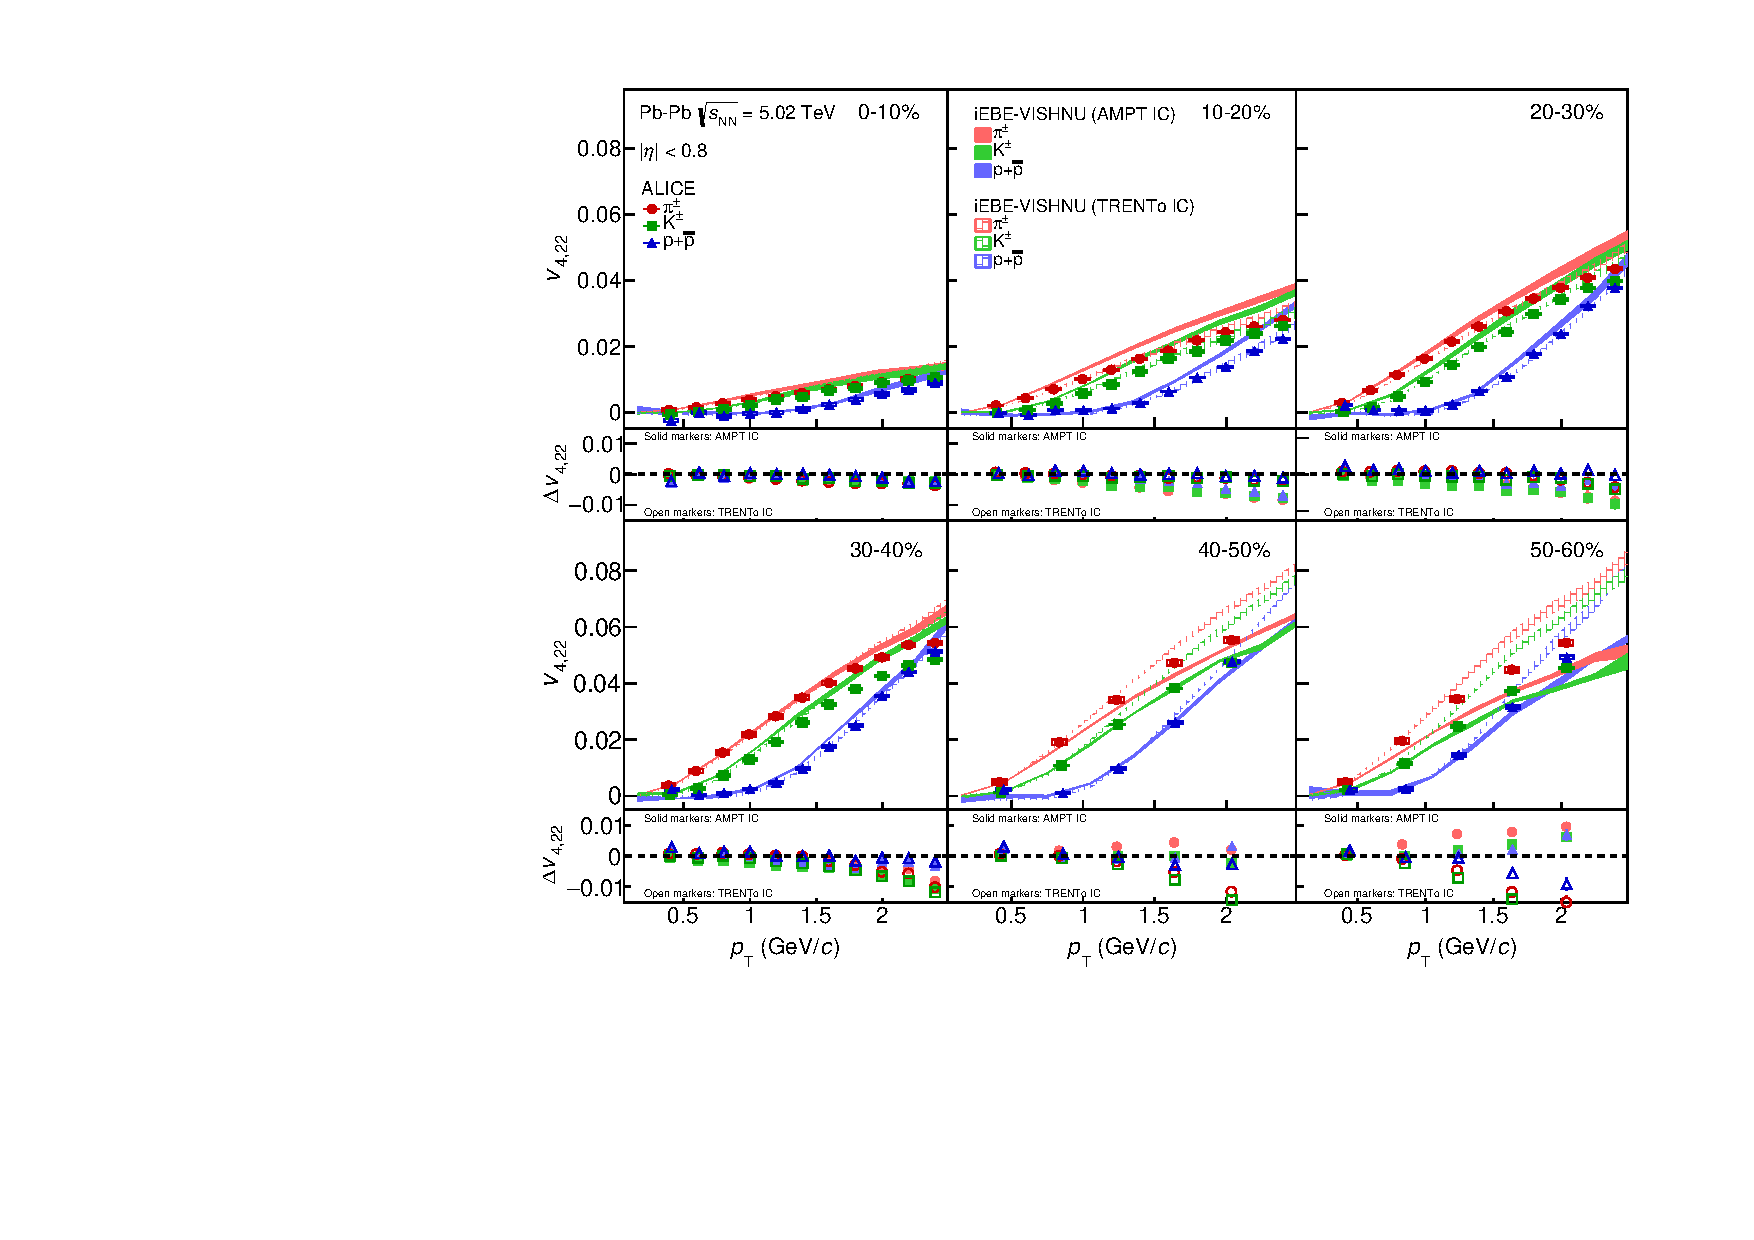
\includegraphics[scale=0.73]{figures/model/TrentoAndAMPT_v422_gap00_PID2.pdf}
\end{center}
\caption{The \pT-differential $v_{4,22}$ for \pion, \kaon~and \proton~in 0-10\% up to 50-60\% centrality intervals of Pb--Pb collisions at \sNN compared with iEBE-VISHNU hybrid models with two different sets of initial parameters: AMPT initial conditions ($\eta/s$= 0.08 and $\zeta/s$ = 0) shown in solid bands and TRENTo initial conditions ($\eta/s({\rm T})$ and $\zeta/s({\rm T})$) in hatched bands. The bottom panels show the difference between the measurements and each model.}
\label{v422_model}
\end{figure}

\begin{figure}[h]
\begin{center}
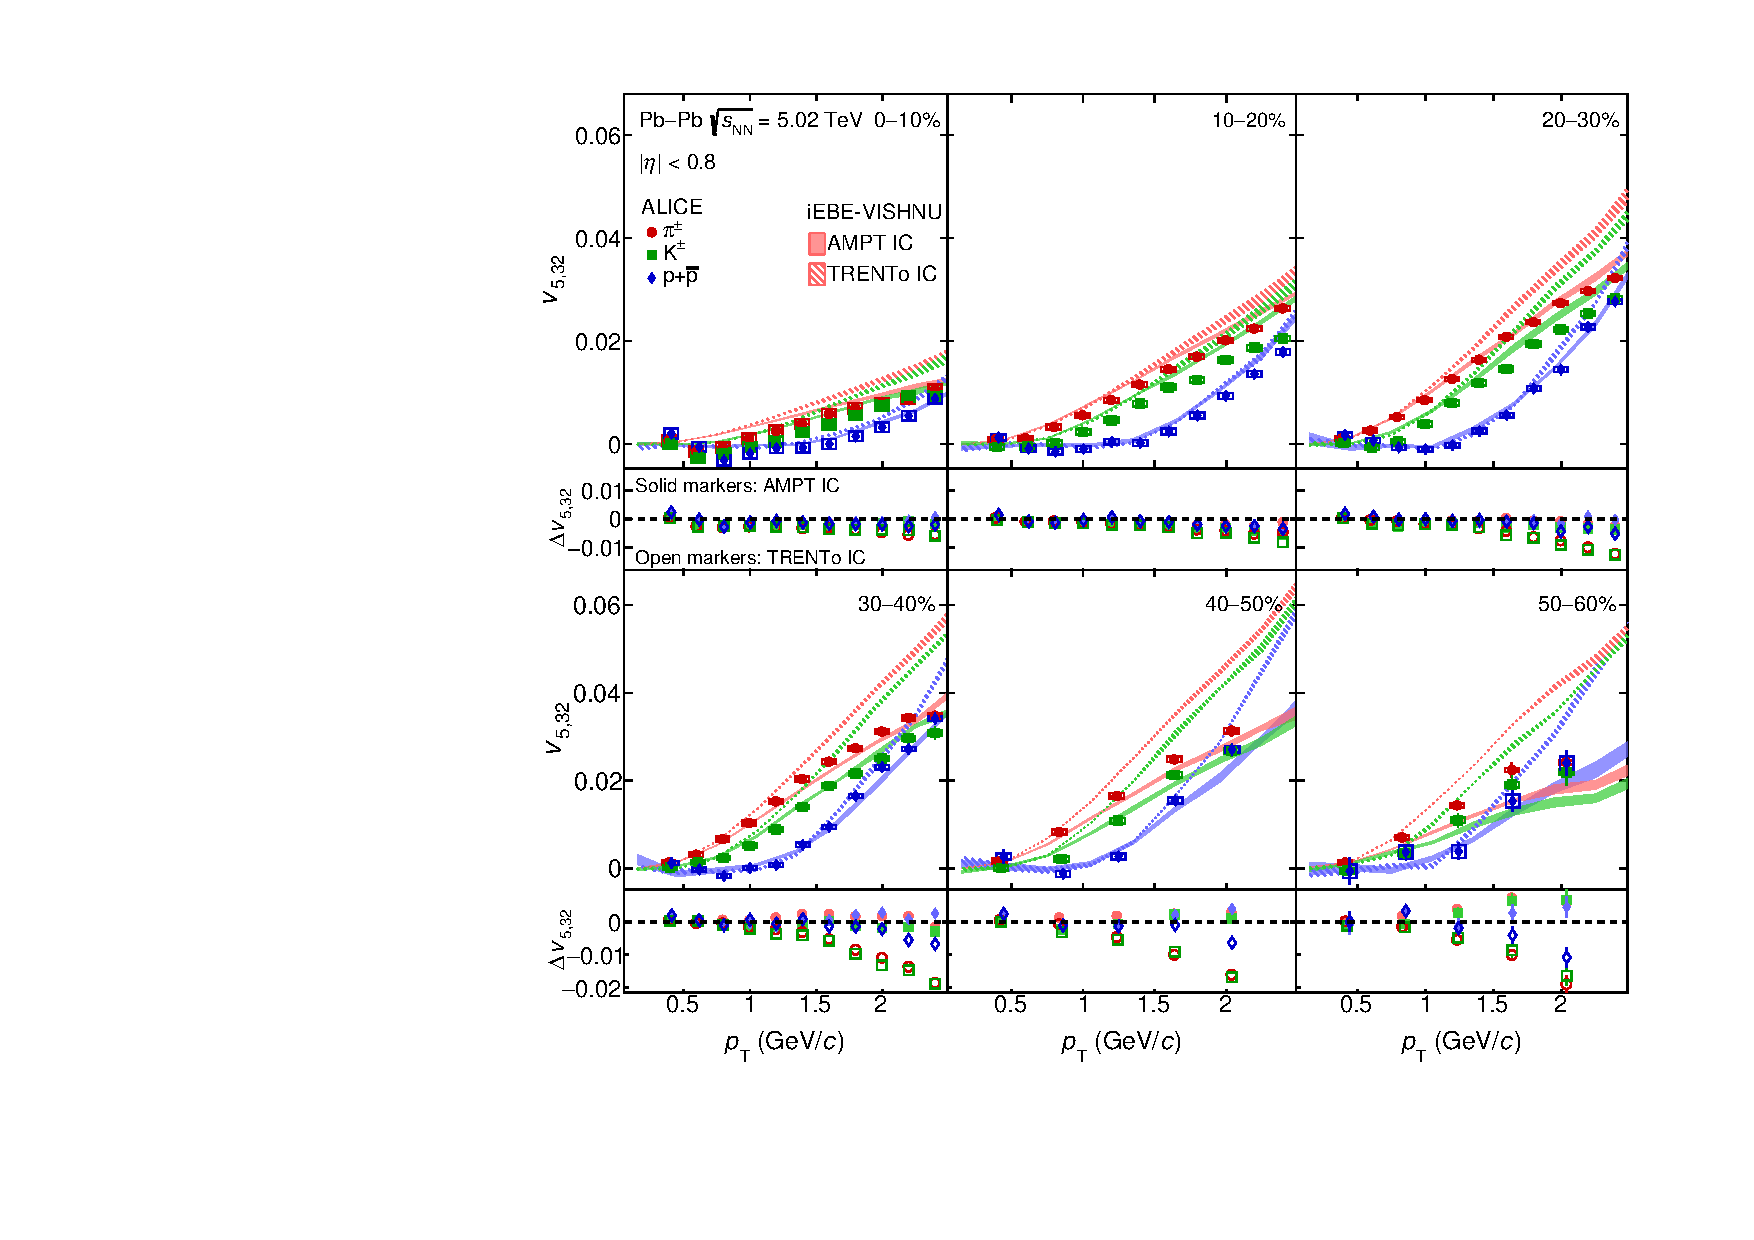
\includegraphics[scale=0.73]{figures/model/TrentoAndAMPT_v523_gap00_PID2.pdf}
\end{center}
\caption{The \pT-differential $v_{5,32}$ for \pion, \kaon~and \proton~in 0-10\% up to 50-60\% centrality intervals of Pb--Pb collisions at \sNN compared with iEBE-VISHNU hybrid models with two different sets of initial parameters: AMPT initial conditions ($\eta/s$= 0.08 and $\zeta/s$ = 0) shown in solid bands and TRENTo initial conditions ($\eta/s({\rm T})$ and $\zeta/s({\rm T})$) in hatched bands. The bottom panels show the difference between the measurements and each model.}
\label{v523_model}
\end{figure}


\begin{figure}[h]
\begin{center}
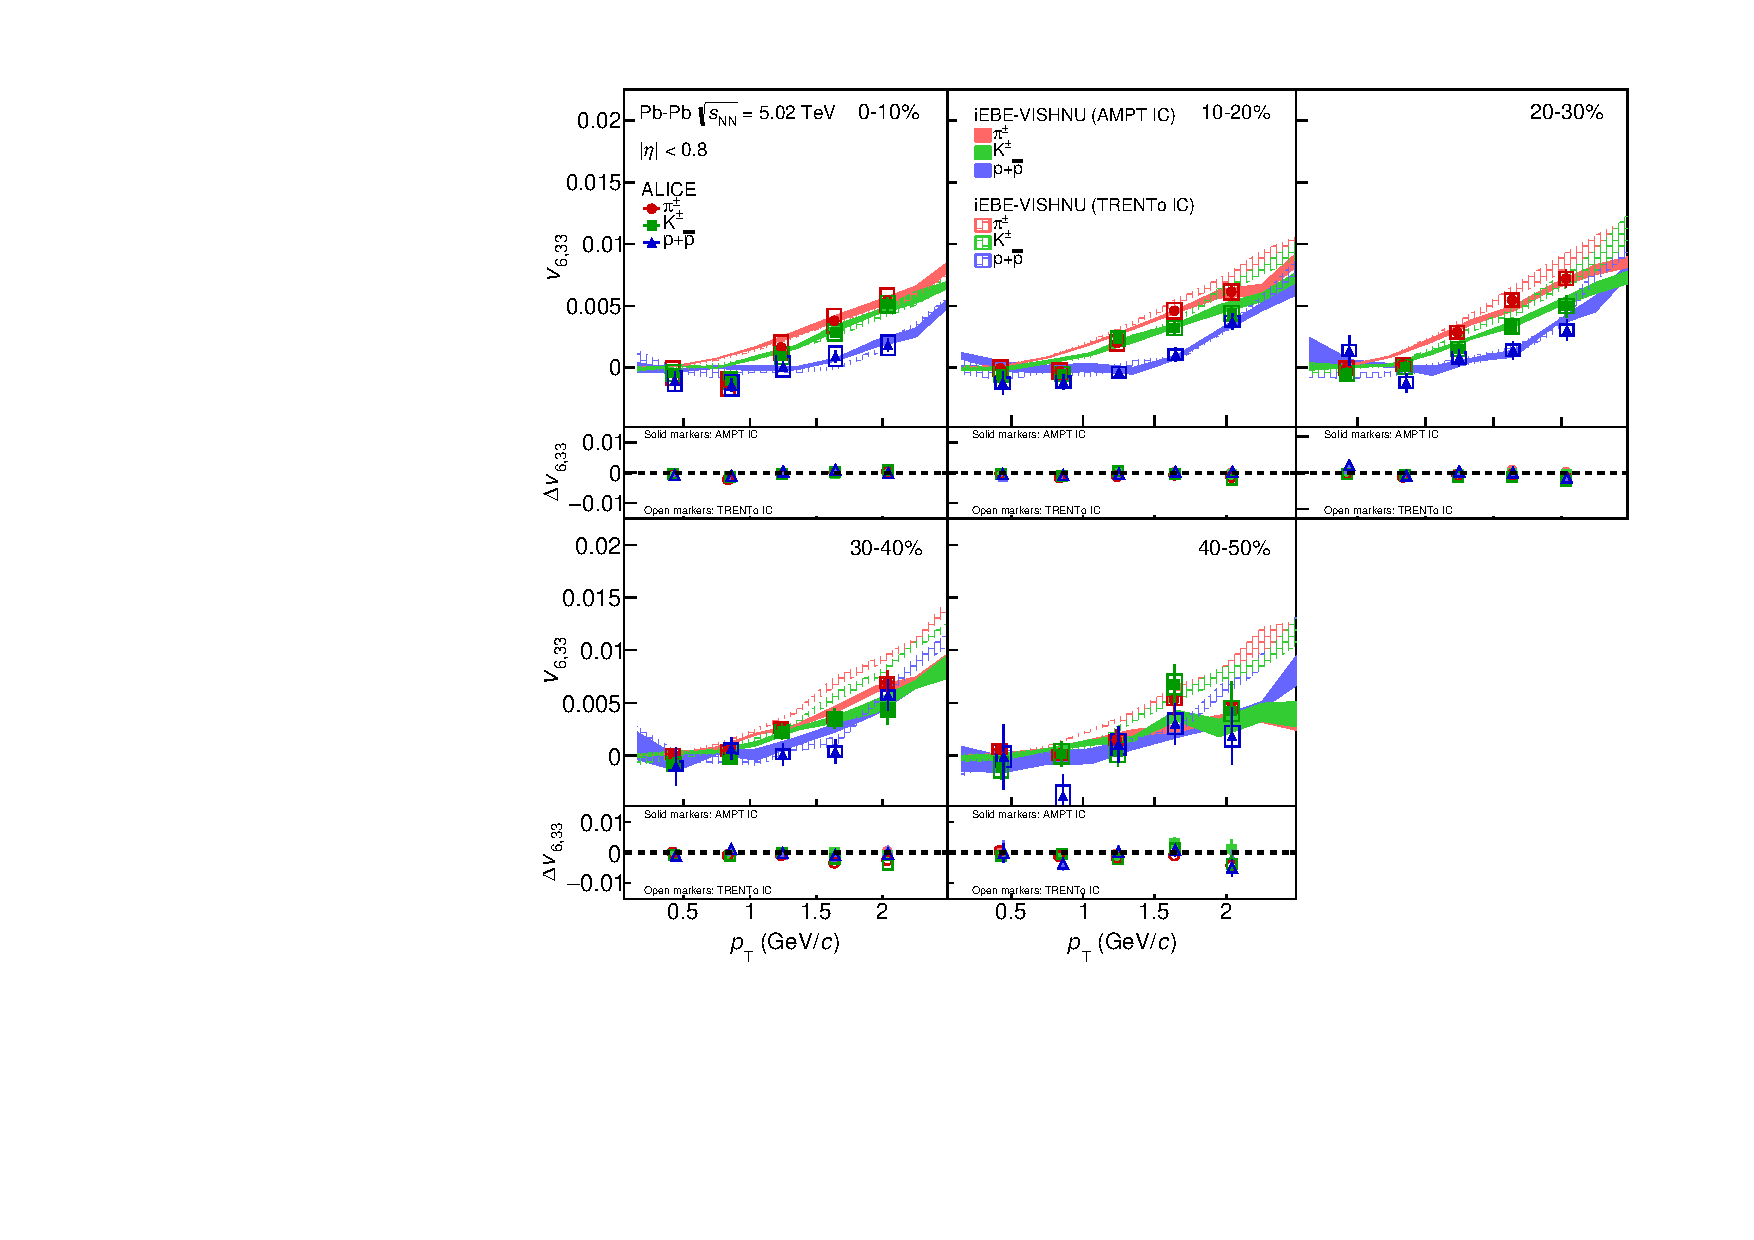
\includegraphics[scale=0.73]{figures/model/TrentoAndAMPT_v633_gap00_PID2.pdf}
\end{center}
\caption{The \pT-differential $v_{6,33}$ for \pion, \kaon~and \proton~in 0-10\% up to 40-50\% centrality intervals of Pb--Pb collisions at \sNN compared with iEBE-VISHNU hybrid models with two different sets of initial parameters: AMPT initial conditions ($\eta/s$= 0.08 and $\zeta/s$ = 0) shown in solid bands and TRENTo initial conditions ($\eta/s({\rm T})$ and $\zeta/s({\rm T})$) in hatched bands. The bottom panels show the difference between the measurements and each model.}
\label{v633_model}
\end{figure}

\begin{figure}[h]
\begin{center}
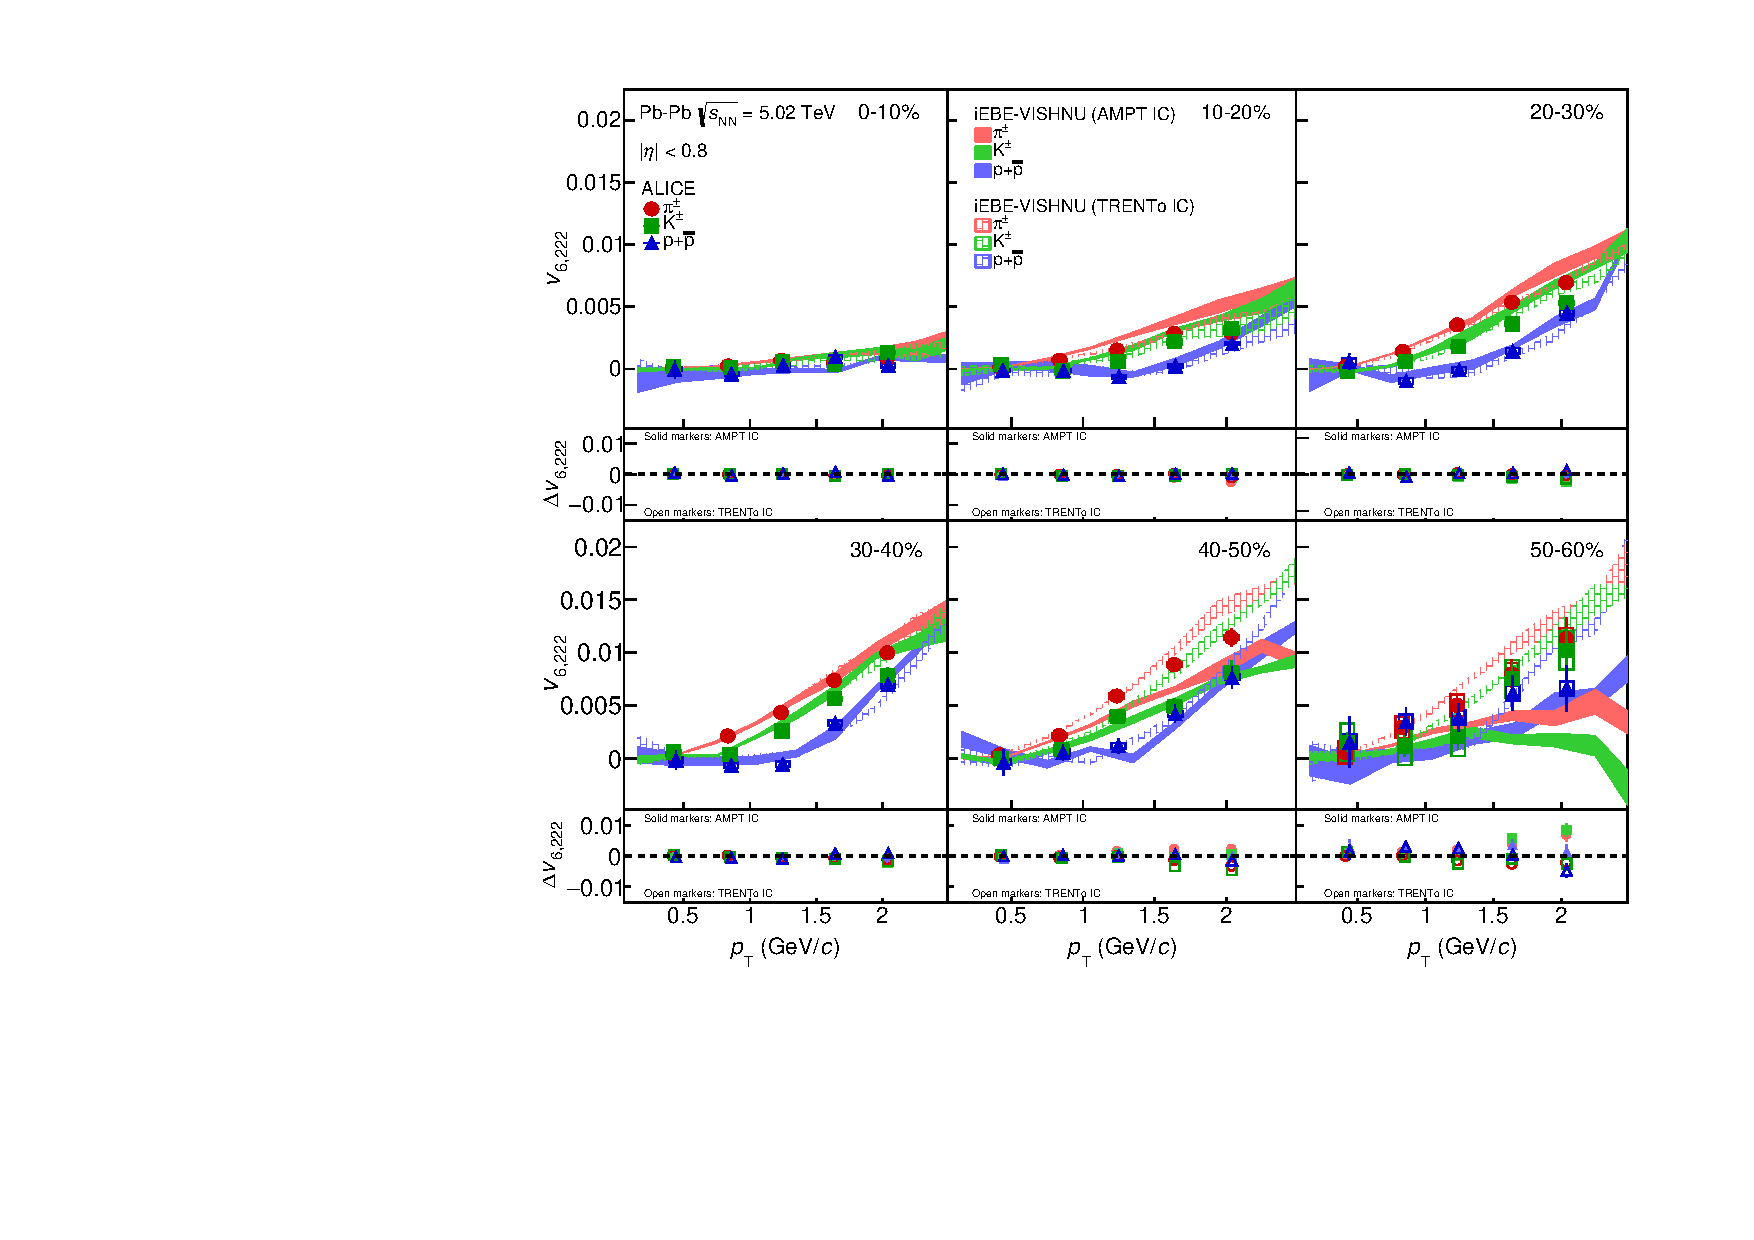
\includegraphics[scale=0.73]{figures/model/TrentoAndAMPT_v6222_gap00_PID2.pdf}
\end{center}
\caption{The \pT-differential $v_{6,222}$ for \pion, \kaon~and \proton~in 0-10\% up to 50-60\% centrality intervals of Pb--Pb collisions at \sNN compared with iEBE-VISHNU hybrid models with two different sets of initial parameters: AMPT initial conditions ($\eta/s$= 0.08 and $\zeta/s$ = 0) shown in solid bands and TRENTo initial conditions ($\eta/s({\rm T})$ and $\zeta/s({\rm T})$) in hatched bands. The bottom panels show the difference between the measurements and each model.}
\label{v6222_model}
\end{figure}



 \begin{figure}[h]
\begin{center}
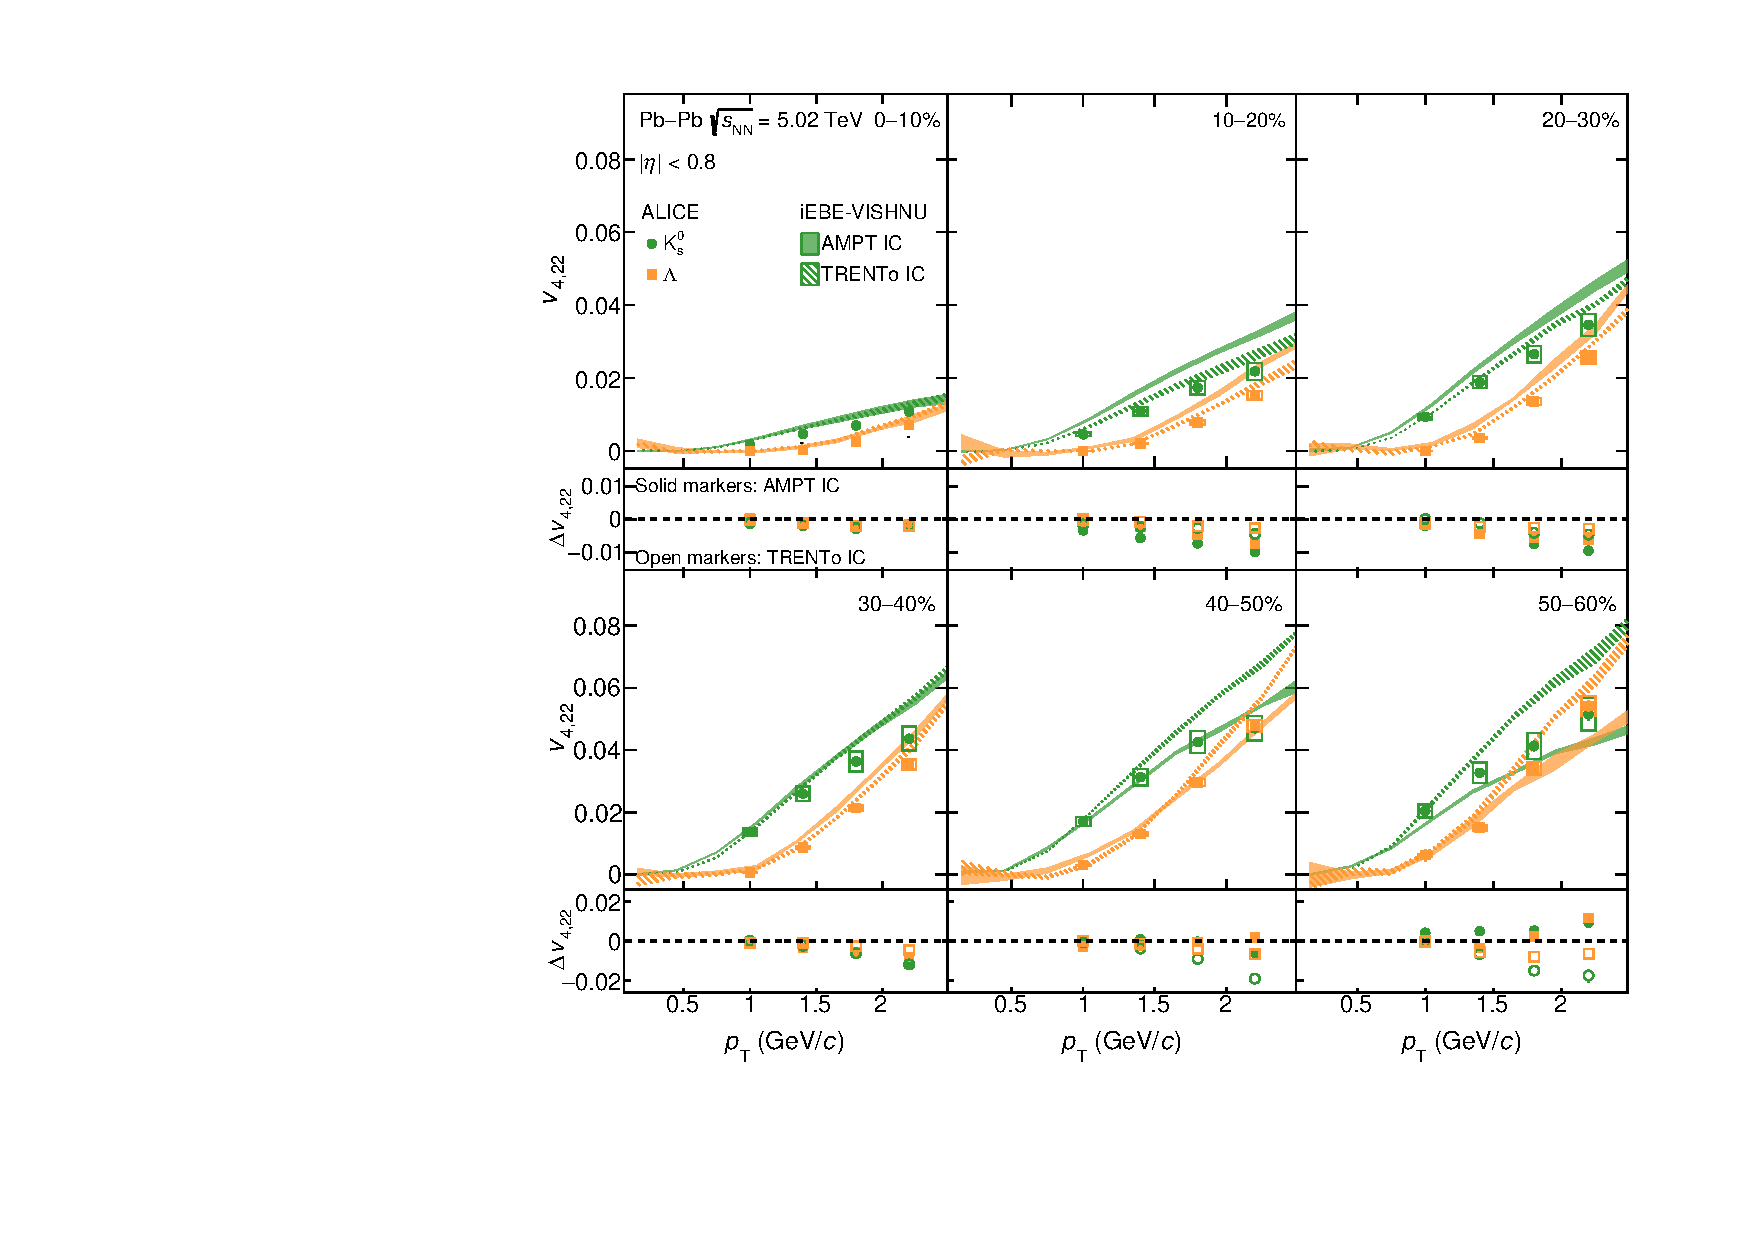
\includegraphics[scale=0.73]{figures/model/TrentoAndAMPT_v422_gap00_LambdaK0s.pdf}
\end{center}
\caption{The \pT-differential $v_{4,22}$ for \Ks~and \lambdas~in 0-10\% up to 50-60\% centrality intervals of Pb--Pb collisions at \sNN compared with iEBE-VISHNU hybrid models with two different sets of initial parameters: AMPT initial conditions ($\eta/s$= 0.08 and $\zeta/s$ = 0) shown in solid bands and TRENTo initial conditions ($\eta/s({\rm T})$ and $\zeta/s({\rm T})$) in hatched bands. The bottom panels show the difference between the measurements and each model.}
\label{v422_model_KL}
\end{figure}


 \begin{figure}[h]
\begin{center}
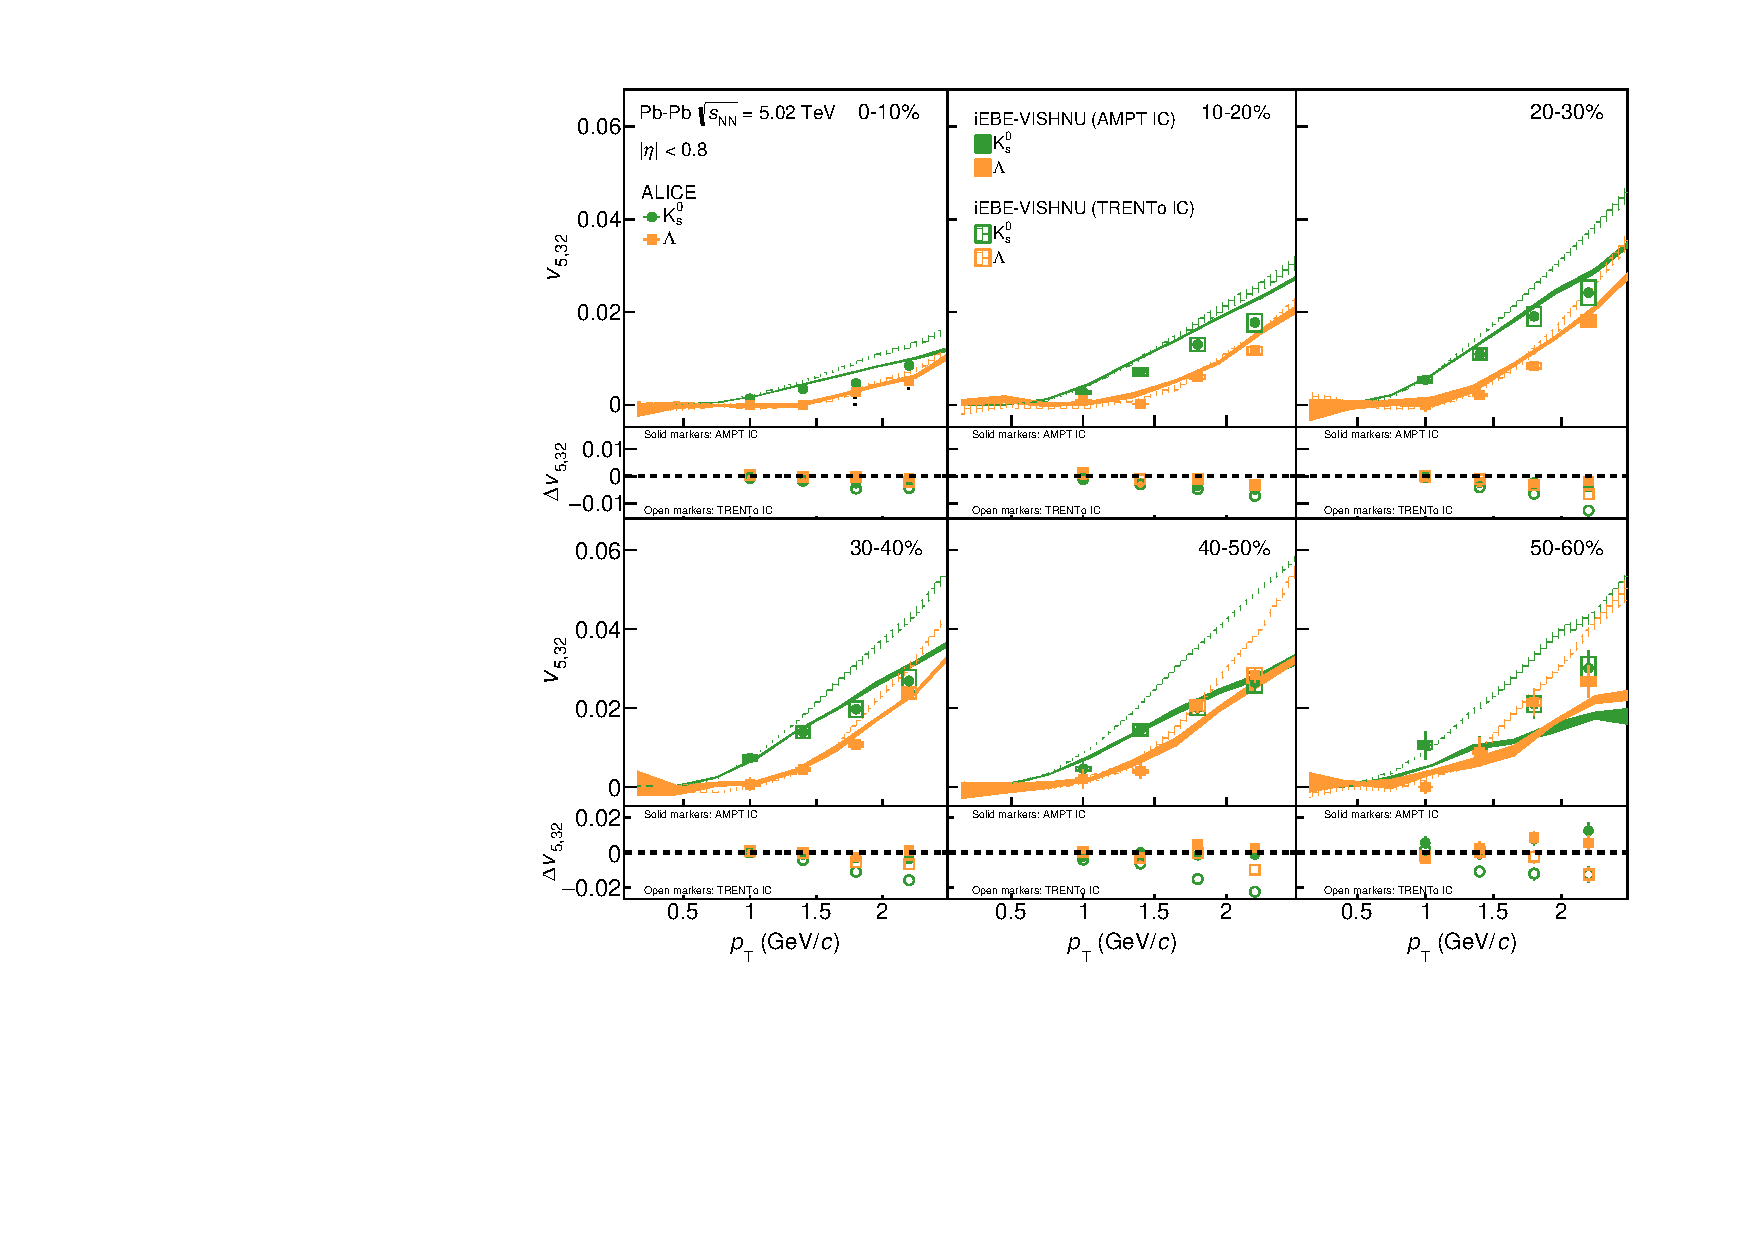
\includegraphics[scale=0.73]{figures/model/TrentoAndAMPT_v523_gap00_LambdaK0s.pdf}
\end{center}
\caption{The \pT-differential $v_{5,32}$ for \Ks~and \lambdas~in 0-10\% up to 50-60\% centrality intervals of Pb--Pb collisions at \sNN compared with iEBE-VISHNU hybrid models with two different sets of initial parameters: AMPT initial conditions ($\eta/s$= 0.08 and $\zeta/s$ = 0) shown in solid bands and TRENTo initial conditions ($\eta/s({\rm T})$ and $\zeta/s({\rm T})$) in hatched bands. The bottom panels show the difference between the measurements and each model.}
\label{v523_model_KL}
\end{figure}


 \begin{figure}[h]
\begin{center}
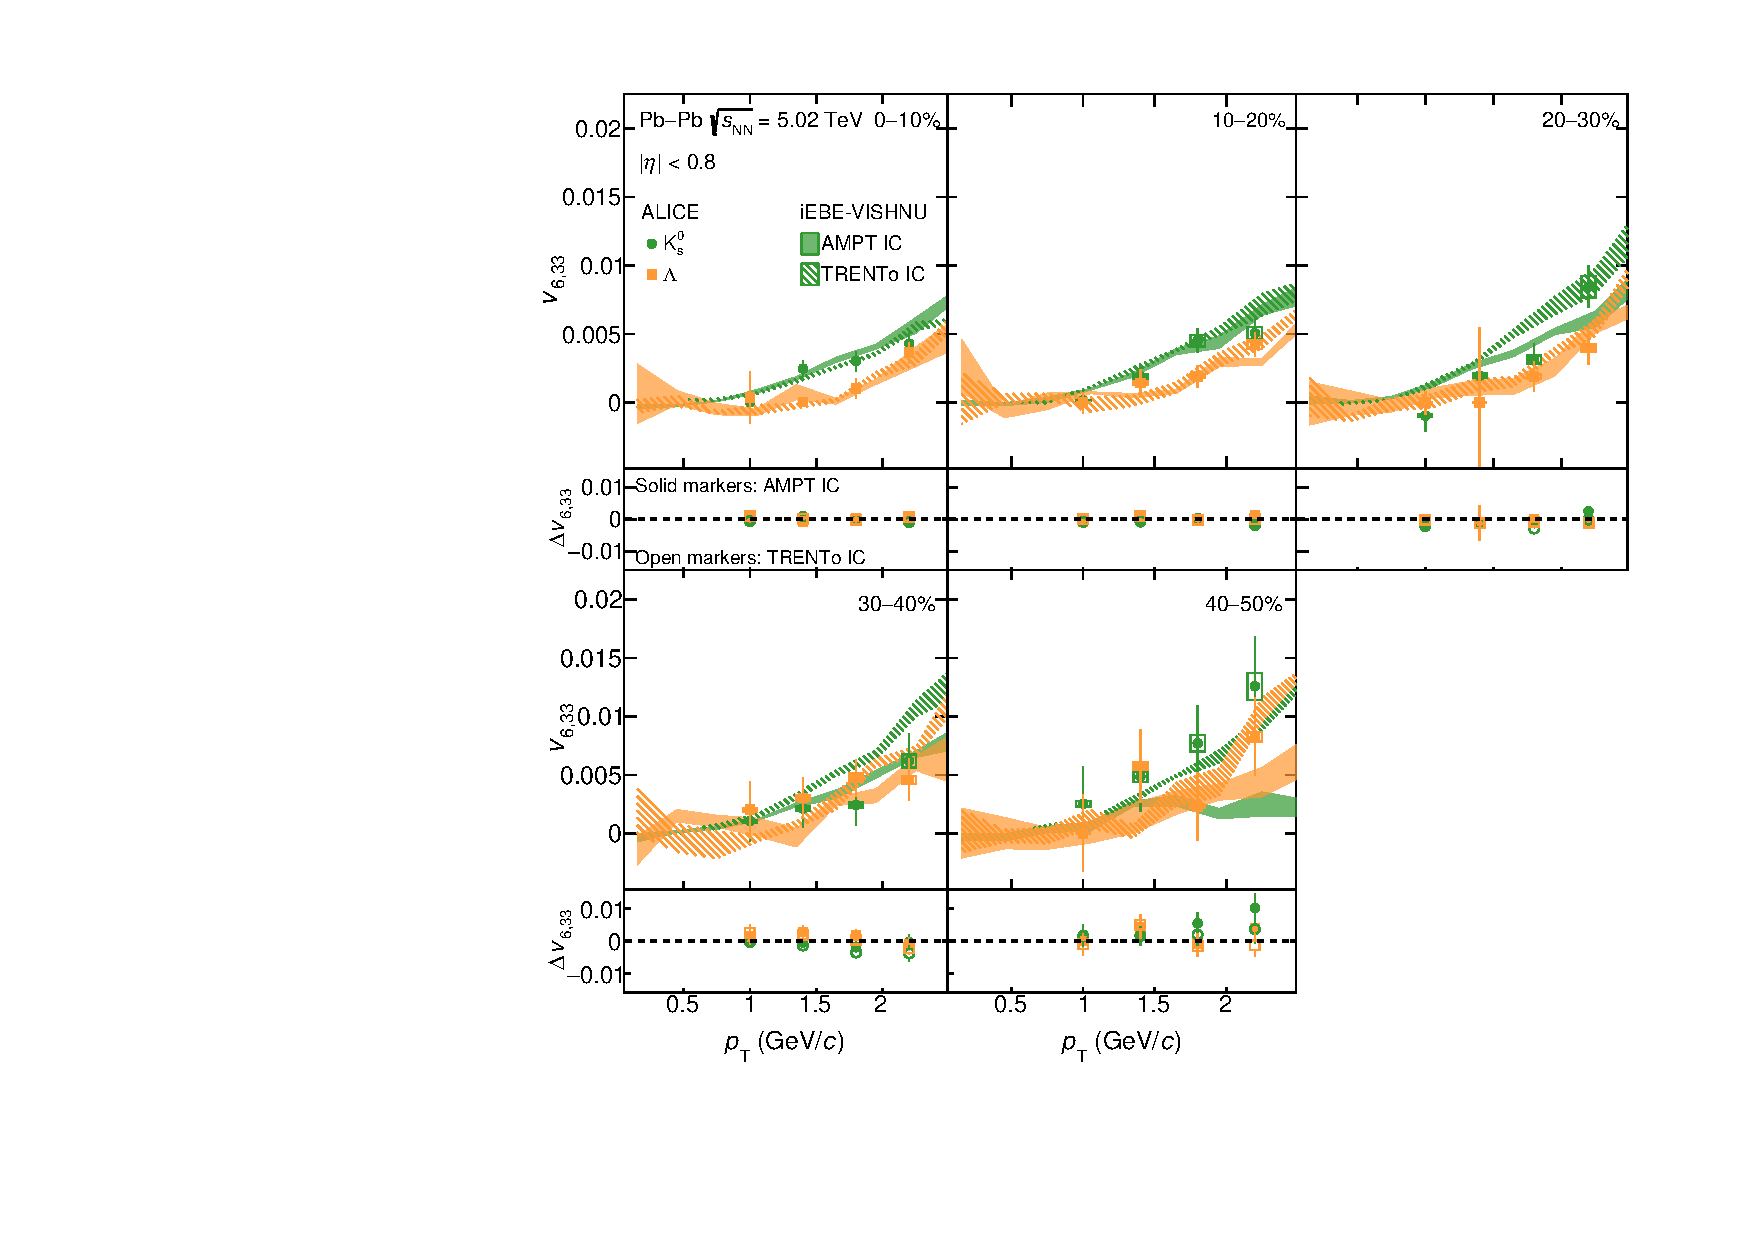
\includegraphics[scale=0.73]{figures/model/TrentoAndAMPT_v633_gap00_LambdaK0s.pdf}
\end{center}
\caption{The \pT-differential $v_{6,33}$ for \Ks~and \lambdas~in 0-10\% up to 40-50\% centrality intervals of Pb--Pb collisions at \sNN compared with iEBE-VISHNU hybrid models with two different sets of initial parameters: AMPT initial conditions ($\eta/s$= 0.08 and $\zeta/s$ = 0) shown in solid bands and TRENTo initial conditions ($\eta/s({\rm T})$ and $\zeta/s({\rm T})$) in hatched bands. The bottom panels show the difference between the measurements and each model.}
\label{v633_model_KL}
\end{figure}


All in all, this study shows larger difference between the model calculations and the $v_{n,mk}$ measurements with respect to that of $v_{n}$, indicating a larger sensitivity to the initial conditions and transport properties for the non-linear flow modes. As a result, it is useful to tune the input parameters of hydrodynamic models considering also the non-linear flow measurements. % and constrain the values of transport properties and the initial conditions of the system.

%All in all, comparing this effort to the data-model comparison for anisotropic flow coefficients \cite{Acharya:2018zuq} shows that non-linear modes are more sensitive to the initial conditions and transport properties. However, similar to model-data comparisons for anisotropic flow, neither of the models can reproduce the data for all centrality intervals and particle species. As a result, in order to constrain the values of transport properties and the initial conditions of the system, it is necessary to tune the input parameters of hydrodynamic models using these measurements.






\newpage